%%%%%%%%%%%%%%%%%%%%%
%   AMS packages    %
%%%%%%%%%%%%%%%%%%%%%
\documentclass{amsart}

\usepackage{amsmath}
\usepackage{amsxtra}
\usepackage{amscd}
\usepackage{amsthm}
\usepackage{amsfonts}
\usepackage{amssymb}
\usepackage{eucal}
\usepackage[all]{xy}
\usepackage{graphicx}
\usepackage{tikz-cd}
\usepackage{mathrsfs}
\usepackage{subfiles}
%\usepackage{mathpazo} not a huge fan
\usepackage{euler}
\usepackage{hyperref}
\usepackage{color}
\usepackage{longtable}
\usepackage{float}
\usepackage{caption}

\usepackage[colorinlistoftodos, textsize=tiny]{todonotes}
\def\listtodoname{List of Todos}
\def\listoftodos{\@starttoc{tdo}\listtodoname}

%\addtolength{\oddsidemargin}{-.5 in}
	%\addtolength{\evensidemargin}{-.4 in}
	%\addtolength{\textwidth}{1 in}
%
	%\addtolength{\topmargin}{0 in}
	%\addtolength{\textheight}{0 in}

\RequirePackage{color}
\definecolor{myred}{rgb}{0.75,0,0}
\definecolor{mygreen}{rgb}{0,0.5,0}
\definecolor{myblue}{rgb}{0,0,0.65}

%\usepackage{hyperref}
  %\hypersetup{colorlinks=true,citecolor=blue}

\usepackage{tikz}
\usepackage{tikz-cd}
\usetikzlibrary{matrix,arrows,decorations.pathmorphing}

%%%%%%%%%%%%%%%%%%%%%%% amsthm theorem styles %%%%%%%%
%%%%%%%%%%%%%%%

\theoremstyle{plain}
  \newtheorem{thm}{Theorem}[section]
  \newtheorem{prop}[thm]{Proposition}
  \newtheorem{lem}[thm]{Lemma}
  \newtheorem{cor}[thm]{Corollary}
	\newtheorem{claim}[thm]{Claim}
	\newtheorem{question}[thm]{Question}
	
\theoremstyle{definition}
  \newtheorem{defn}[thm]{Definition}
  \newtheorem{example}[thm]{Example}
  \newtheorem{exer}[thm]{Exercise}
  \newtheorem{ctexample}[thm]{Counterexample}
  \newtheorem{convention}[thm]{Convention}
	\newtheorem{conjecture}[thm]{Conjecture}
	
\theoremstyle{remark}
	\newtheorem{rem}[thm]{Remark}
  \newtheorem{note}[thm]{Notation}
  \newtheorem*{note*}{Notation}
  \newtheorem{case}{Case}
	
\numberwithin{equation}{section}

%%%%%%%%%%%%%%%%%%%%%%%%% custom commands %%%%%%%%%%%%%%%%%%%%%%%%%%%

\newcommand\nc{\newcommand}
\nc\on{\operatorname}
\nc\renc{\renewcommand}
\newcommand\ssec{\subsection}
\newcommand\sssec{\subsubsection}
\newcommand\BH{{\mathbb H}}
\newcommand\BN{{\mathbb N}}
\newcommand\BC{{\mathbb C}}
\newcommand\BF{{\mathbb F}}
\newcommand\BR{{\mathbb R}}
\newcommand\BQ{{\mathbb Q}}
\newcommand\BP{{\mathbb P}}
\newcommand\BZ{{\mathbb Z}}
\newcommand\BA{{\mathbb A}}
\newcommand\Bk{{\Bbbk}}

\newcommand\sco{{\mathscr O}}

\newcommand{\id}{\mathrm{id}}
\newcommand\im{\text{im }}
\newcommand\coker{\text{coker}}
\newcommand\spec{\text{Spec }}
\newcommand\proj{\text{Proj }}
\newcommand\gal{\mathrm{Gal}}

\DeclareMathOperator{\ord}{ord}
\DeclareMathOperator{\sym}{Sym}

%%%%%%%%%%%%%%%%%%%%% cring custom commands %%%%%%%%%%%%%%%%%%%%%%%%%

\DeclareMathOperator\di{Div}
\newcommand\sx{\mathscr X}
\newcommand \subhalf[1]{\frac{{#1} - 1}{2{#1}}}
\newcommand{\se}[1]{\section*{Problem #1}}
\newcommand{\halfcan}{L}
\DeclareMathOperator{\Supp}{Supp}
\DeclareMathOperator{\initial}{in_\prec}
\DeclareMathOperator{\gin}{gin}
\DeclareMathOperator{\Eff}{Eff}
\DeclareMathOperator{\sat}{sat}
\DeclareMathOperator{\newspan}{span}
\captionsetup[table]{belowskip = 4pt}

\newcommand{\GL}{\operatorname{GL}}
\newcommand{\SL}{\operatorname{SL}}
\newcommand{\PGL}{\operatorname{PGL}}
\newcommand{\PSL}{\operatorname{PSL}}

\renewcommand{\arraystretch}{1.2}

\makeatletter
\newcommand{\customlabel}[2]{%
   \protected@write \@auxout {}{\string \newlabel {#1}{{#2}{\thepage}{#2}{#1}{}} }%
   \hypertarget{#1}{#2}
}
\makeatother

%%%%%%%%%%%%%%%%%%%%%%%%%%%%%% title %%%%%%%%%%%%%%%%%%%%%%%%%%%%%%%%

\title{Canonical rings of log spin stacky curves}

\author{Aaron Landesman}
\address[Aaron Landesman]{Department of Mathematics, Harvard University}
\email{aaronlandesman@college.harvard.edu}

\author{Peter Ruhm}
\address[Peter Ruhm]{Department of Mathematics, Stanford University}
\email{pruhm@stanford.edu}

\author{Robin Zhang}
\address[Robin Zhang]{Department of Mathematics, Stanford University}
\email{robinz16@stanford.edu}

\date{\today}

%%%%%%%%%%%%%%%%%%%%%%%%%%%%% document %%%%%%%%%%%%%%%%%%%%%%%%%%%%%%

\begin{document}

\begin{abstract}
 	Consider modular forms arising from finite-area
	quotients of the upper-half plane by Fuchsian groups.  
	By the classical results of Kodaira--Spencer, 
	this space of modular forms may be
	viewed as log spin canonical ring of a stacky curve.
	In this paper, we tightly bound the degrees of minimal
	generators and relations of log spin canonical rings and,
	as a consequence, 
	obtain a tight bound on the degrees of minimal generators and relations  		
	for rings of modular forms of arbitrary integral weight.
\end{abstract}

\maketitle

\todo{Think about John's comment to regrade the ring.}

%%%%%%%%%%%%%%%%%%%%%%%%%%%% Introduction %%%%%%%%%%%%%%%%%%%%%%%%%%%%%%%

\section{Introduction}
Let $\Gamma$ be a {\bf Fuchsian group}, i.e.,~ a discrete subgroup of
$\PSL_2(\BR)$ acting on the upper half plane $\BH$ by fractional
linear transformations, such that $\Gamma \backslash \BH$ has finite area.
We consider the graded {\bf ring of modular forms}
$M(\Gamma) = \bigoplus_{k = 0}^\infty M_k(\Gamma)$. One of the best ways to describe the ring $M(\Gamma),$ is to write down a presentation.
%of $M(\Gamma)$ for general Fuchsian groups $\Gamma$. 
To do so, it is useful to have a bound on the
degrees in which the generators and relations can occur. In the
special case that $\Gamma$ has no odd weight modular forms, Voight
and Zureick-Brown give tight bounds \cite[Chapters 7-9]{vzb:stacky}.
We extend their result to all Fuchsian groups $\Gamma$ in the main
theorem of this work.

We can now consider the orbifold $\Gamma \backslash \BH$ over $\BC$.
For example, in the case $\Gamma$ acts freely on $\BH$, $\Gamma
\backslash \BH$ is a Riemann Surface over $\BC$. 
$\Gamma \backslash \BH$ may be non-compact, but in such cases we can form a
compact Riemann Surface, $\Gamma \backslash \BH^*,$ by adding in
cusps, with associated divisor of cusps $\Delta$.

In order to find generators and relations for $M(\Gamma)$, we
translate the seemingly analytic question of understanding the ring
of modular forms into the algebraic category, using a
generalization of the GAGA principle.
 By \cite[Proposition 6.1.5]
{vzb:stacky}, there is an equivalence of categories between orbifold
curves and log stacky curves over $\BC$. Hence, for the remainder
of the paper, we will work in the algebraic category.

Let $X$ be a smooth proper geometrically-integral algebraic curve of genus $g$ over a field $\Bk$.
It is well known that the canonical sheaf $\Omega _X,$ with
associated canonical divisor $K_X$, determines the {\bf canonical
map } $\pi: X \rightarrow \BP_\Bk^{g - 1}$. Then, the {\bf canonical
ring} is defined to be
\begin{align*}
	R(X, K_X) = \bigoplus_{k \geq 0} H^0(X, kK_X),
\end{align*}

\noindent
with multiplication structure corresponding to tensor product of
sections. In the case that $g \geq 2$, $\Omega_X$ is ample, so $X
\cong \proj R$. When $g \geq 2$, Petri's theorem gives generators
and relations for $R(X, K_X)$ showing that in most cases $R(X, K_X)$
is generated in degree 1 with relations in degree 2, as shown in
\cite[p. 157]{saint-donat:proj} and Arbarello--Cornalba--Griffiths--Harris
\cite[Section 3.3]{acgh:algebraic-curves}. This has the pleasant 
geometric consequence that all such canonically embedded curves are
scheme theoretically cut out by degree 2 equations.

Following Voight and Zureick-Brown \cite{vzb:stacky}, we generalize 
Petri's theorem in the direction of stacky curves equipped with
log divisors. For a stacky curve $\sx$ with coarse space $X$ and
stacky points (also called ``fractional points'') $P_1, \ldots, P_r$
with stabilizer orders $e_1, \ldots, e_r \in \BZ_{\geq 2}$, we define

\[
	\di \sx = \left(\bigoplus_{P\notin \{P_1, \ldots, P_r\}} \langle 
	P \rangle \right) \oplus \left(\bigoplus_{i = 1}^r \left \langle 
	\frac{1}{e_i}P_i \right \rangle \right) \subseteq \BQ \otimes \di X.
\]
Then a {\bf log spin curve} is a triple $(\sx, \Delta, \halfcan)$
where $\Delta \in \di X$ is a log divisor and $L \in \di \sx$ satisfies $2\halfcan \sim K_X +
\Delta + \sum_{i = 1}^{r} \subhalf{e_i} P_i$. The central object of
study in this paper is the {\bf log spin canonical ring} of $(\sx,
\Delta, \halfcan),$ notated as
\begin{align*}
	R(\sx, \Delta, \halfcan) = \bigoplus_{k \geq 0} H^0(X, \lfloor k \halfcan \rfloor).
\end{align*}

\noindent
A brief overview of stacky curves, log divisors, and log spin
canonical rings is given in Subsection
~\ref{ssec:stacky-background}.

%If $X$ is a curve, \todo{why do you start with a curve and then
%move to a stacky curve? shouldn't it be the opposite order?} then
%we say $\sx$ is a {\bf stacky curve} with {\bf coarse space} $X$
%and {\bf stacky points} (also called {\bf{fractional points}}) $P_1,
%\ldots, P_r$ with {\bf stabilizer orders} $e_1, \ldots, e_r \in \BZ_{
%\geq 2}$ if 
%\[
	%\di \sx = \left(\bigoplus_{P\notin \{P_1, \ldots, P_r\}} \langle 
	%P \rangle \right) \oplus \left(\bigoplus_{i = 1}^r \left \langle 
	%\frac{1}{e_i}P_i \right \rangle \right) \subseteq \BQ \otimes \di X
%\]

%A {\bf log spin curve} is a triple $(\sx, \Delta, \halfcan)$ where
%$\Delta \in \di X$ is a log divisor and $2\halfcan = K_X +
%\Delta + \sum_{i=1}^{r} \subhalf{e_i} P_i.$
%The central object of study in this paper is the {\bf log spin
%canonical ring} of $(\sx, \Delta, \halfcan)$ is
%\begin{align*}
	%R(\sx, \Delta, \halfcan) = \bigoplus_{d \geq 0} H^0(X, d \halfcan)
%\end{align*}

In particular, we bound the degrees of generators and relations of
a log spin canonical ring. Let $\sx$ be a stacky curve with
signature $\sigma = (g; e_1, \ldots, e_r; \delta)$. The application
of O'Dorney's work \cite[Chapter 5]{dorney:canonical} to log spin
canonical rings gives a weak bound in the case $g = 0$ in terms of
the least common multiples of the $e_i$'s. In their treatment of
log spin canonical rings, Voight and Zureick-Brown
\cite[Corollary 10.4.6]{vzb:stacky} bounded generator degrees by $6
\cdot \max(e_1, \ldots, e_r)$ and relation degrees by $12 \cdot \max
(e_1, \ldots, e_ r)$ when $\halfcan$ is effective. Note that the
bounds we write here differ from those stated in Voight and Zureick-
Brown \cite[Corollary 10.4.6]{vzb:stacky} by a factor of 2 because
their grading convention differs from ours by a factor of 2.

These bounds are far from tight and do not collectively
cover all cases in all genera. The main theorem of this paper
gives significantly tighter bounds for the log spin canonical ring
of any log spin curve.

\begin{thm}
\label{thm:main}
Let $(\sx, \Delta, \halfcan)$ be a log spin curve over a perfect
field $\Bk$, so that $\sx$ has signature $\sigma = (g; e_1, \ldots,
e_r; \delta)$.

Then the log spin canonical ring is generated as a $\Bk$-algebra by 
elements of degree at most $e = \max(5, e_1, \ldots, e_r)$ with
relations generated in degrees at most $2e$,
so long as $\sigma$ does not lie in a finite list of exceptional
cases, as given in Table ~\ref{table:g-1-exceptional} for
signatures with $g = 1$ and Table ~\ref{table:g-0-exceptional} for
signatures with $g = 0$.
\end{thm}

\begin{rem}
\label{rem:main-weaker-assumptions}
In fact, the proof of Theorem ~\ref{thm:main} holds with $\Delta$ replaced by an arbitrary effective divisor of the coarse space.
 Furthermore, one may relax the assumption that $\Bk$ is perfect. Instead, one only need assume that the stacky curve
is separably rooted, as described further in Remark ~\ref{rem:stack-formalism}.
\end{rem}

Theorem ~\ref{thm:main} is proven separately in the cases that the genus $g = 0, g = 1,$ and $g \geq 2$ in Theorems ~\ref{thm:g-0-main}, ~\ref{thm:g-1-main}, and ~\ref{thm:g-high-main}, respectively.  In each of these proofs, we follow a similar inductive process utilizing the lemmas of Section ~\ref{sec:induction}; however, in the first two we have to explicitly construct specific base cases and present a finite list of exceptional cases, while in the genus $g \geq 2$ case we deduce base cases from more general arguments.
\begin{rem}
\label{rem:explicit-generators}
The main theorem obtains bounds on the degrees of the generators
and relations of log spin canonical rings. However, the proof
of the genus one and genus zero cases also yield explicit systems
of generators and an explicit initial ideal of relations.
Furthermore, our proof of the genus $g \geq 2$ case also provides
an inductive procedure for explicitly determining the generators
and initial ideal of relations of log spin canonical rings. Many
explicit systems of generators and relations for curves of genus $2
\leq g \leq 15$ are detailed in interesting examples by Neves
\cite[Section III.4]{neves:halfcan}. 
\end{rem}
\begin{rem}
The explicit construction described in Remark ~\ref{rem:explicit-generators} also reveals that the bounds given in Theorem ~\ref{thm:main} are tight.
Specifically, in almost all cases, the log spin canonical ring requires a generator in degree $e = \max(5, e_1, \ldots, e_r)$ and a relation in degree at least $2e-4$. 
Furthermore, there are many infinite families of cases which require a generator in degree $e = \max(5, e_1, \ldots, e_r)$ and a relation in degree exactly $2e$. \todo{Explain this in more detail later, as asked by Brian}
\end{rem}

Combining the main theorem of this paper, Theorem ~\ref{thm:main} with the main theorem from Voight and Zureick-Brown ~\cite
[Theorem 1.4]{vzb:stacky} and a minor Lemma \cite[Lemma 10.2.1]{vzb:stacky}
we have the following application to
rings of modular forms.
%Note that the lemma from Voight and Zureick-
%Brown ~\cite[Lemma 10.2.1]{vzb:stacky} follows almost immediately
%from the classical work of Kodaira--Spencer
%\cite{kodaira-spencer:deformations}.

\begin{cor}
\label{cor:main-mod-forms}
Let $\Gamma$ be a Fuchsian group and $\sx$ the stacky curve
associated to $\Gamma \backslash \BH$ with signature $\sigma
= (g; e_1, \ldots, e_r; \delta)$. 

If $M_k(\Gamma) = 0$ for all odd $k$, then the ring of modular
forms $M(\Gamma)$ is generated as a $\BC$-algebra by elements of
degree at most $6 \cdot \max(3, e_1, \ldots, e_r)$ with relations
generated in degrees at most $12 \cdot \max(3, e_1, \ldots, e_r)$.

If there is some odd $k$ for which $M_k(\Gamma) \neq 0$, then the
ring of modular forms $M(\Gamma)$ is generated as a $\BC$-algebra
by elements of degree at most $\max(5, e_1, \ldots, e_r)$ with
relations generated in degree at most $2 \cdot \max(5, e_1, \ldots, 
e_r)$ so long as $\sigma$ does not lie in a finite list of
exceptional cases which are listed and described in Table
~\ref{table:g-1-exceptional} for signatures with $g = 1$ and in
Table ~\ref{table:g-0-exceptional} for signatures with $g = 0$.
\end{cor}

\begin{rem}
\label{rem:gen-at-most-three}
If $M(\Gamma)$ has some odd weight modular form, then it has an odd weight modular form in weight $3$. When $g \geq 2$, we see that this is true because $\dim_k H^0(\sx, 3\halfcan) > 0$ by Riemann--Roch and the fact that $\deg \lfloor 3\halfcan \rfloor > 2g - 1$. When the genus is zero or one, we see that there is a generator in weight $1$ or weight $3$ in the base cases given in Table ~\ref{table:g-1-base} and Table ~\ref{table:g-0-base-cases} so there is an odd weight modular form in weight $3$ in general. A consequence of this observation is that the bound on the degree of generators and relations when $M(\Gamma)$ has some odd weight modular form, as given in Corollary ~\ref{cor:main-mod-forms}, is closely related to the degree of the minimal odd weight modular form.
\end{rem}

\begin{example}
\label{eg:congruence-bounds}
Suppose $\Gamma \subset SL_2(\BZ)$ is a congruence subgroup. Then, since 
the action  of $SL_2(\BZ)$ has points with stabilizer order 2 and 3, the 
action of $\Gamma$ can only have points with stabilizer order 2 and 3. 
Furthermore, if $\Gamma$ has some odd weight modular form, then it must 
have no points with stabilizer order 2 (see Remark ~\ref{rem:odd-denom}). 
Therefore, by Corollary ~\ref{cor:main-mod-forms}, $M(\Gamma)$ is 
generated in degree at most $5$ with relations in degree at most $12$. 
Furthermore, if the coarse space associated $\Gamma$ does not have, 
$(0;3,3,3,3;0),$ there are relations in degree at most $10$, as follows 
from the list of exceptional cases in Tables ~\ref{table:genus-0-exceptional-cases} and ~\ref{table:genus-0-exceptional}.
\end{example}


\begin{rem}
\label{rem:factor-two}
In the case that $M_k(\Gamma) = 0$ for all odd $k$, the generation bound of $6 \cdot \max(3, e_1, \ldots, e_r)$ and relation
bound of $12 \cdot \max(3, e_1, \ldots, e_r)$ can be reduced to $2\cdot \max(3,e_1, \ldots, e_r)$ and $4 \cdot \max(3,e_1, \ldots, e_r)$, apart from several small families of cases. See 
~\cite[Theorem 9.3.1]{vzb:stacky} and ~\cite[Theorem 8.7.1]{vzb:stacky} for a more precise statement of these bounds in the cases that $g = 0$ and $g > 0$ respectively. Note that we multiply all bounds given in Voight and Zureick-Brown \cite{vzb:stacky} by a factor of two. Our grading convention for log spin canonical rings uses weight $k$ for the degree whereas Voight and Zureick-Brown $d = 2k$ for degree.
\end{rem}


The remainder of the paper will be primarily devoted to proving
Theorem ~\ref{thm:main}. The idea of the
proof will be to induct first on the number of stacky points and then on the stabilizer order of those points.  To this end, we first review important background in
Section ~\ref{sec:background}; providing essential examples in Section \ref{sec:examples}; develop various inductive
tools in Section ~\ref{sec:induction}; and prove Theorem ~\ref{thm:main} in genus $g\ge 2$, genus $g=1$, and genus $g=0$ in Sections ~\ref{sec:g-high},
~\ref{sec:g-1}, and ~\ref{sec:g-0} respectively.  
Finally, in Section
~\ref{sec:further-questions}, we pose several questions for future
research.

%%%%%%%%%%%%%%%%%%%%%%%%%%%% Background %%%%%%%%%%%%%%%%%%%%%%%%%%%%%%%

\section{Background}
\label{sec:background}
Here we collect various definitions and notation that will be
used throughout the paper. Many of the conventions come from existing
literature. For basic references on the statements and definitions
used below, see Hartshorne \cite[Chapter IV]{hartshorne:ag},
Saint-Donat \cite{saint-donat:proj}, Arbarello--Cornalba--Griffiths--Harris 
\cite[Section III.2]
{acgh:algebraic-curves}, and Voight--Zureick-Brown \cite[Chapter 2,
Chapter 5]{vzb:stacky}.

For the remainder of this paper, fix an algebraically closed field $\Bk$.
This is no restriction on generality, as generator and relation degrees are preserved under base change to the algebraic closure.

\ssec{Stacky Curves and Log Spin Canonical Rings}
\label{ssec:stacky-background}
We begin by setting up the notation for stacky curves and canonical rings. Wherever possible, we opt for a more elementary scheme-theoretic approach, instead of a stack-theoretic one. See Remark ~\ref{rem:stack-formalism} for more details.

\begin{defn}
\label{defn:stacky-curve}
A \textbf{stacky curve} $\sx$ over an algebraically closed field $\Bk$ is the datum of a smooth proper integral scheme $X$ of dimension $1$, together with a finite number of closed points of $X$, $P_1, \ldots, P_r$, called {\bf stacky points}, with {\bf stabilizer orders} $e_1, \ldots, e_r \in \BZ_{\geq 2}.$ The scheme $X$ associated to a stacky curve $\sx$ is called the {\bf coarse space} of $\sx$.
\end{defn}

\begin{rem}
\label{rem:stack-formalism}
Stacky curves may be formally defined in the language of stacks, as
is done in the works of Voight and Zureick-Brown \cite{vzb:stacky},
Abramovich and Vistoli \cite{abramovich-vistoli:compactifying}, and
Behrend and Noohi \cite{behrend-noohi:uniformization}.

The results of this paper can be easily couched in terms of the language of stacks. If one works over an arbitrary field $\Bk$ (which need not be algebraically closed) one can extend Theorem ~\ref{thm:main} to hold in the case that the stacky curve $\sx$ is tame and separably rooted, i.e.,~ the residue field of each
of the stacky points is separable.

With this stack-theoretic description in mind, the remainder of this paper is primarily phrased using the language
of schemes.
\end{rem}

\begin{defn}
\label{defn:div-ex}
Let $\sx$ be a stacky curve over $\Bk$ with coarse space $X$ of genus $g$ and stacky points $P_1, \ldots,
P_r$ with stabilizer orders $e_1, \ldots, e_r \in \BZ_{\geq 2}$.
Then, we notate
\[
	\di \sx = \left(\bigoplus_{P\notin \{P_1, \ldots, P_r\}} \langle 
	P \rangle \right) \oplus \left(\bigoplus_{i = 1}^r \left \langle 
	\frac{1}{e_i}P_i \right \rangle \right) \subseteq \BQ \otimes \di X.
\]
\end{defn}

We can equip stacky curves with a log divisor $\Delta$ that is a 
sum of distinct points each with trivial stabilizer. 
A divisor
$\Delta$ of this form is called a \textbf{log divisor}. We use
$\delta := \deg \Delta$ to refer to the degree of the log divisor.
If $\sx$ has coarse space $X$ of genus $g$, then we say $\sx$ has
\textbf{signature} $\sigma = (g; e_1, \ldots, e_r; \delta)$.

\begin{defn}
\label{defn:divisor-floor}
If divisor $D \in \di \sx$ and $D = \sum_{i = 1}^{n} \alpha_i P_i$
with $\alpha_i \in \BQ$, the floor of a divisor $\lfloor D
\rfloor$ is defined to be $\lfloor D \rfloor := \sum_{i = 1}^{n}
\lfloor \alpha_i \rfloor P_i$.
\end{defn}

A pair of a stacky curve and a log divisor $(\sx, \Delta)$ is
called a \textbf{log stacky curve} and the study of their
canonical rings is the main focus of the work by Voight and 
Zureick-Brown \cite{vzb:stacky}. For this paper, we consider \textbf{log
spin curves} which are triples $(\sx, \Delta, \halfcan)$ where $\sx$
is a stacky curve, $\Delta$ is a log divisor, and $\halfcan \in \di
\sx$ satisfies $2 \halfcan \sim K_X + \Delta + \sum_{i = 1}^{r}
\frac{e_i - 1}{e_i} P_i$. Such a divisor $\halfcan$ is called a
\textbf{log spin canonical divisor} on $(\sx, \Delta)$. Throughout the paper, we use
the notation $\halfcan_X := \lfloor L \rfloor.$ to refer to the log spin
canonical divisor (also known as the half-canonical divisor, 
semi-canonical divisor, or theta characteristic) associated to the
coarse space $X$ of $\sx.$  (i.e.,~ $\halfcan_X$ is a divisor such
that $2\halfcan_X \sim K_X + \Delta$). 
We define $H^0$ of a stacky divisor as follows.

\begin{defn}
\label{defn:h0-stacky}
Recall the standard notation 
$$\sco(D) = \{f \in \Bk(X)^\times : \di f + D \geq 0 \}.$$
Let $\sx$ be a stacky curve with coarse space $X$.
If $D \in \di \sx$ is a Weil divisor, then we define
\begin{align*}
	H^0(\sx, D) &:= H^0(X, \lfloor D \rfloor)\\
	H^0(\sx, \sco(D)) &:= H^0(\sx, D)\\
	h^0(\sx, \sco(D)) &:= \dim_\Bk H^0(\sx, \sco(D))
\end{align*}
If $R$ is a graded ring, then we let $(R)_k$ refer to the $k^\text{th}$
graded component of $R$.

\end{defn}

\begin{rem}
Although Definition ~\ref{defn:h0-stacky} may seem fairly ad hoc, it is naturally motivated in the context of stacks. See Voight and Zureick-Brown \cite[Lemma 5.4.7]{vzb:stacky} for a proof that Definition ~\ref{defn:h0-stacky} is equivalent to the stack-theoretic description.
\end{rem}

\begin{defn}
\label{defn:log-spin-canonical-ring}
The {\bf log spin canonical ring} of $(\sx, \Delta, \halfcan)$ is
\[
	R(\sx, \Delta, \halfcan) = \bigoplus_{k \geq 0} H^0(\sx, k \halfcan).
\]
\end{defn}

\noindent
When the log spin curve is fixed, we usually use $R$ or $R_\halfcan$ to
represent $R(\sx, \Delta, \halfcan)$.

\begin{rem}
\label{rem:odd-denom}
Suppose $(\sx, \Delta, L)$ is a log spin curve. Note that
\[
	\halfcan = \sum_{i = 1}^{r} \subhalf{e_i} P_i + \sum_{i = 1}^{s} a_i Q_i
\]

\noindent
where $a_i \in \BZ$ and $e_i$ are odd. This is due to the fact
that $\halfcan \in \di \sx$: 
if some $e_i$ were even,
then $\frac{e_i - 1}{2e_i}$ would be in reduced form implying $\halfcan \notin \di \sx$.
\end{rem}
	
\begin{rem}
\label{rem:delta-not-1}
Suppose $(\sx, \Delta, \halfcan)$ is a log spin curve. Note that $\deg \Delta$
is even. because $2 \cdot \deg \halfcan = \deg \Delta + \deg \lfloor K
\rfloor = \deg \Delta + 2(g-1).$
In particular, we shall often use $\deg \Delta \neq 1$.
\end{rem}

\ssec{Saturation}

We define the notion of the saturation of a divisor, as can be found in
Voight and Zureick-Brown ~\cite[Section 7.2]{vzb:stacky}.

\begin{defn}
Let $D$ be a divisor on $\sx$. The \textbf{effective monoid} of $D$
is the monoid
\[
	\Eff(D) = \{k \in \BZ_{\geq 0} : \deg \lfloor kD \rfloor \geq 0 \}.
\]
\end{defn}

\begin{defn}
\label{defn:sat}
The \textbf{saturation} of a monoid $M \subseteq \BZ_{\geq 0}$,
denoted $\sat(M)$, is the smallest integer $s$ such that $M
\supseteq \BZ_{\geq s}$, if such an integer exists.
\end{defn}

\begin{rem}
For $D \in \di \sx$, we will often call $\sat(\Eff(D))$ the saturation of $D.$
\end{rem}

\ssec{Monomial Ordering}
\label{ssec:monomial-order}
Here we give a brief overview of the three monomial orderings
that we use. For further reference on monomial orderings,
initial ideals, and Gr\"{o}bner bases, see Eisenbud
\cite[Section 15.9]{eisenbud:comm-alg} and Cox--Little--O'Shea
\cite[Chapter 2]{cls:ideals-varieties-algorithms}.

\begin{defn}
\label{defn:monomial-degree}
Let $\Bk[x_1$, $\ldots$, $x_n]$ be a graded polynomial
ring with $\deg x_i = k_i$ and let $\alpha := \prod_{i = 1}^{n} x_{i}^{f_i} \in
\Bk[x_{1}$, $\ldots$, $x_{n}]$ be a monomial. Then
we define the {\bf degree} of $\alpha$ to be
\[
	\deg \alpha := \sum_{i = 1}^{n} k_i f_i.
\]
\end{defn}

\begin{defn}
\label{defn:grevlex}
The {\bf graded reverse lexicographic order}, or {\bf grevlex} $\prec_{\text{grevlex}}$ is defined as follows.
If $\alpha := \prod_{i = 1}^{n} x_{i}
^{f_i}$ and $\beta := \prod_{i = 1}^{n} x_{i}^{f_i'}$ are
monomials in $\Bk[x_{1}$, $\ldots$, $x_{n}]$, then $\alpha
\succ_{\text{grevlex}} \beta$ if either

\begin{equation}
	\deg \alpha = \sum_{i = 1}^{n} k_i f_i  > \sum_{i = 1}^{n} k_i f_i' = \deg \beta
\end{equation}
or
\begin{equation}
\label{eqn:grevlex-tie}
	\deg \alpha = \deg \beta \text{ and }	f_i < f_i' \text{ for
	the	largest } i \text{ such that } f_i \neq f_i'.
\end{equation}
\end{defn}

\begin{rem}
Note that the ordering of the variables matters in Equation
~\ref{eqn:grevlex-tie}.
\end{rem}

Our inductive arguments in Section ~\ref{sec:induction} will
usually have an inclusion $R \supseteq R'$ of log spin canonical
rings such that $R_\halfcan$ is generated by elements $x_{i}$ and $R$
is generated over $R_{\halfcan'}$ by elements $y_j$. In these cases, it is
natural to consider term orders which treat these sets of variables
separately.

\begin{defn}
\label{defn:block-order}
The \textbf{block term order} is defined as follows. Let $\Bk[y_{1}, \ldots, y_{m}]$ and $\Bk[x_{1}, \ldots,
x_{n}]$ be weighted polynomial rings with $\deg y_i = c_i, \: \deg x_i = k_i.$ Further assume we are given existing term
orders $\prec_y$ and $\prec_x$. Let $\alpha :=
\prod_{j = 1}^{m} y_{j}^{h_i}$ $\prod_{i = 1}^{n} x_{i}
^{f_i}$ and $\beta := \prod_{j = 1}^{m} y_{j}^{h_i'}
\prod_{i = 1}^{n} x_{i}^{f_i'}$ be monomials in $\Bk[y_{1},
\ldots, y_{m}] \otimes$ $\Bk[x_{1}, \ldots, x_{n}]$.
Let $\alpha_y := \prod_{j = 1}^{m} y_{j}^{h_i}$ be the
part of $\alpha$ in $\Bk[y_{1}, \ldots, y_{m}]$ and
likewise with $\alpha_x$, $\beta_y$, and $\beta_x$.

In the \textbf{(graded) block} (or \textbf{elimination}) term
ordering on $\Bk[y_{k_1', 1}, \ldots, y_{k_m', m}] \otimes \Bk[x_{k_1, 1},
\ldots, x_{k_n, n}]$, we define $\alpha \succ \beta$ if
  \begin{enumerate}
	\item[(i)] $\deg \alpha  > \deg \beta$ or
  \item[(ii)] $\deg \alpha = \deg \beta$ and $\alpha_y \succ_y \beta_y$ or
	\item[(iii)] $\deg \alpha = \deg \beta$ and $\alpha_y = \beta_y$ and $\alpha_x \succ_x \beta_x$.
  \end{enumerate}
\end{defn}

Now we give brief definitions of initial terms and Gr\"{o}bner
bases. These will be used in the proofs of the inductive lemmas
in Section ~\ref{sec:induction} as well as in the proof of Theorem
~\ref{thm:main}.

\begin{defn}
\label{defn:initial-term}
Let $\prec$ be an ordering on $\Bk[x_{1}$, $\ldots$, $x_{n}]$, 
with $\deg x_i = k_i$,
and let $f \in \Bk[x_{1}, \ldots, x_{n}]$ be a homogeneous
polynomial. The \textbf{initial term} $\initial(f)$ of $f$
is the largest monomial in the support of $f$ with respect to
the ordering $\prec$. Furthermore, we set $\initial(0) := 0$.
\end{defn}


\begin{defn}
\label{defn:initial-ideal}
Let $I$ be a homogeneous ideal of $\Bk[x_{1}$, $\ldots$,
$x_{n}]$. Then the {\bf initial ideal} $\initial(I)$ of $I$ is
the ideal generated by the initial terms of homogeneous polynomials
in $I$:
\[
	\initial(I) := \langle \initial(f) \rangle_{f \in I}
\]
\end{defn}

%Furthermore, we will use Gr\"{o}bner bases, which are bases
%for these initial ideals and have many useful properties.

\begin{defn}
\label{defn:grobner-basis}
Let $I$ be a homogeneous ideal of $\Bk[x_{1}$, $\ldots$,
$x_{n}]$. A \textbf{Gr\"obner basis} for $I$, also known as a
\textbf{standard basis} for $I$, is a set of elements in $I$
such that their initial terms generate the initial
ideal of $I$.
\end{defn}

\ssec{Admissibility}

Here, we define a notion of admissibility that is quite similar to the admissibility defined by Voight and Zureick-Brown \cite[Definition 8.5.1]{vzb:stacky}. Our notion is an adaptation the case of log spin canonical divisors.

One key difference between the notion of admissibility in Definition ~\ref{defn:admissible} and that of Voight and Zureick-Brown \cite[Definition 8.5.1]{vzb:stacky} is that 
%in \cite{vzb:stacky}, Voight and Zureick-Brown may assume that $\{P_i\} \cap \Supp(K_X) = \emptyset.$ 
we cannot assume that $\{P_i\} \cap \Supp(L_X') = \emptyset$, as $H^0(X, \halfcan_X')$ may have no global sections. We circumvent this issue by working with the orders of zeros and poles relative to $\halfcan_X'$, rather than relative to the $\sco_X$.

\begin{defn}
\label{def:order-sup}
Let $D \in \di \sx.$ If $z$ is a rational section of $\sco(D)$ denote the order of
zero of $z$ at $P$ by $\ord_P^D(z)$.
\end{defn}

\begin{defn}
\label{defn:admissible}
Let $(\sx', \Delta, L')$ be a log spin
curve, with coarse space $X$ and stacky points $Q_1, \ldots, Q_r$.  Let $J \subset
\{1, \ldots, r\}$. Let $e_i := e_i'+ 2 \chi_J (i)$ where

\[
\chi_J(i) = \begin{cases}
	1, &\text{ if }i \in J\\
	0, &\text{ otherwise. } 
\end{cases}
\]

Let $R'$ be the canonical ring associated to $\sx'$. Define $(\sx', \halfcan', J)$
to be {\bf admissible} if $R'$ admits a presentation
\begin{align*}
	R' \cong \left( \Bk[x_1, \ldots, x_m] \otimes \Bk[y_{i, e_i'}]_{i \in J} \right)/I'
\end{align*}

\noindent
with each $y_{i, e_i'}$ viewed in $R'$ through the image of this isomorphism and such that for each $i \in J$ such that the following
three conditions hold:
\begin{enumerate}
	\item[\customlabel{custom:Ad-i}{(Ad-i)}] First, 
		\begin{align*}
		\deg y_{e_i'} &= e_i'  &\text{ and } &&-\ord_{Q_i}^{\halfcan_X'}(y_{i, e_i'})
			= \frac{e_i'- 1}{2}.
		\end{align*}
	\item[\customlabel{custom:Ad-ii}{(Ad-ii)}] Second, every generator $z 
		\in \{x_1, \ldots, x_m\} \cup \{y_{j, e_i'}: j\in J - \{i\} \}$ 
		satisfies
		\begin{align*}
			\frac{-\ord_{Q_i}^{\halfcan_X'}(z)}{\deg z} < \subhalf {e_i'}.
		\end{align*}
	\item[\customlabel{custom:Ad-iii}{(Ad-iii)}] Third, we have
		\begin{align*}
			\deg \lfloor e_i L' \rfloor \geq \max(2g - 1,0) + \max_{k \geq 0} \# S_{\sigma, J}(i, k)
		\end{align*}
		where
		\begin{align*}
			S_{\sigma, J}(i, k) := \{j \in J : j \neq i \text{ and } e_j'+2k
			\mid e_i - e_j'\}.
		\end{align*}
\end{enumerate}
\end{defn}

%%%%%%%%%%%%%%%%%%%%%%%%%%% Examples %%%%%%%%%%%%%%%%%%%%%%%%%%%%%%%

\section{Examples}
\label{sec:examples}

In this section, we work out several examples of computing presentations for spin canonical rings. In several cases, we also check certain triples are admissible, as defined in Definition ~\ref{defn:admissible}. In addition to providing intuition for the lemmas of Section ~\ref{sec:induction}, these examples also serve as useful base cases for our inductive proof of Theorem ~\ref{thm:main}.

\begin{example}
\label{eg:base-1-0}
Let $(\sx',0, \halfcan')$ be a log stacky curve of genus $g = 1,$ with $\halfcan' = 0$.
Counting dimensions, we see $h^0(\sx, k\halfcan')=1$ for all $k \in \mathbb{Z}_{\ge 0}$ so it is immediately clear that $R_{\halfcan'} \cong \Bk[x]$ with $x$ a generator in degree 1.
\end{example}


\begin{example}
\label{eg:adding-point}
Let $\sx$ be a stacky curve with coarse space $X$ and signature $(0
; 3; 3)$. Let $P_1$ denote the lone stacky point which has stabilizer
order $3$ and suppose $\infty$ is a fixed closed point of $X$ that is
not equal to $P_1$.

We will deduce the structure of the log spin canonical ring $R_L$
from the structure of the spin canonical ring $R_{L_X} := R(X, 3
\cdot \infty, L_X)$. This technique will later be generalized in Lemma ~\ref{lem:sat-1}.

Note that $R_{L_X} \cong \Bk[x_1, x_2]$ where $\deg x_1 = \deg x_2 = 1.
$ To see this, observe that we will need two generators in degree $1$
because $h^0(X, L_X) = 2$ by Riemann--Roch. Because $L_X$ is very 
ample, we have that $R_{L_X}$ is generated in degree 1. To
conclude, note that $R_{L_X}$ does not have any relations. If there
exists some relation, then $\dim \proj R_{L_X} < 1$. This would
contradict the fact that $L_X$ is very ample. Thus, $\proj R_{L_X}
\cong X$ which has dimension 1.

Next, we construct generators and relations for $R_L$ using those
of $R_{L_X}$. Note that we have a natural inclusion $\iota: R_{L_X}
\hookrightarrow R_L$ induced by the inclusions $H^0(\sx, k\halfcan_X)
\hookrightarrow H^0(\sx, k\halfcan)$ for each $k \geq 0$. By Riemann Roch,
we see there is some element $y_{1, 3} \in (R_L)_3$ with $\ord_{P_1}
(y_{1, 3}) = -1$, not in the image of the inclusion $\iota$. We
claim that there exist $a_1, a_2 \in \Bk$ and a degree $4$ polynomial
$f(x_1, x_2) \in \Bk[x_1, x_2]$ such that
\begin{align*}
	R_L \cong \Bk[x_1, x_2, y_{1, 3}] / (a_1 x_1 y_{1, 3} + a_2 x_2 y_{1, 3}
	+ f(x_1,x_2))
\end{align*}

First, note that $x_1, x_2, y_{1, 3}$ generate all of $R_L$ from the
Generalized Max Noether Theorem for genus zero curves from Voight
and Zureick-Brown \cite[Lemma 3.1.1]{vzb:stacky}. That is, the maps
\begin{align*}
	H^0(\sx, 3L) \otimes H^0(\sx, (k - 3)L) \rightarrow H^0(\sx, k\halfcan)
\end{align*}

\noindent
are surjective for $k \geq 4$. A relation of the form $a_1 x_1 y_{1,
3} + a_2 x_2 y_{1, 3} + f(x_1, x_2) = 0$ must exist because $h^0(\sx,
4L) - h^0(\sx, 4L_X) = 1,$ but $x_1 y_{1, 3}$ and $x_2 y_{1, 3}$
define two linearly independent elements with nontrivial image in
the 1-dimensional vector space $H^0(\sx, 4L) / H^0(\sx, 4L_X).$ So,
we obtain a surjection
\begin{align}
\label{align:surjection}
	\Bk[x_1, x_2, y_{1, 3}] / (a_1 x_1 y_{1, 3} + a_2 x_2 y_{1, 3} + f(x_1, x_2)) 
	\rightarrow R_L.
\end{align}

To complete the example, it suffices to show there are no
additional relations. First, note that $a_1 x_1 y_{1, 3} + a_2 x_2
y_{1, 3} + f(x_1, x_2)$ is irreducible because there are no
relations among $x_1, x_2$ and $y_{1, 3}$ in lower degrees. Hence,
$\Bk[x_1, x_2, y_{1, 3}] / (a_1 x_1 y_{1, 3} + a_2 x_2 y_{1, 3} +
f(x_1, x_2))$ is integral and is 2-dimensional. Thus, the map
\eqref{align:surjection} defines a surjection from an integral
2-dimensional ring to a 2-dimensional ring. Therefore, it is an 
isomorphism.
\end{example}


\begin{example}
\label{eg:base-0-377}
Let $(\sx', 0, \halfcan')$ be a log spin curve with signature $\sigma =
(0; 3, 7, 7; 0)$ and $\halfcan' \sim -\infty + \frac{1}{3} P_1 +
\frac{3}{7} P_2 + \frac{3}{7} P_3,$ where $P_1, P_2,$ and $P_3$ are
distinct points. In this example, we will exhibit a minimal
presentation for $R' = R(\sx', 0, \halfcan')$ and show the triple
$(\sigma, \halfcan' + \frac{3}{7} P_3, J = \{2, 3\},$) is admissible.
Notice that $\deg \lfloor k K_{\sx'} \rfloor= -k + \lfloor \frac{k}{3}
\rfloor + 2 \lfloor \frac{3k}{7} \rfloor$.

By the Generalized Max Noether Theorem for genus 0 curves (see Voight
and Zureick-Brown \cite[Lemma 3.1.1]{vzb:stacky}),
\begin{align}
\label{eqn:noether-377}
	H^0 (\sx', 21 \cdot \halfcan') \otimes H^0 (\sx',
	(k - 21) \halfcan') \rightarrow H^0 (\sx',
	k \halfcan')
\end{align}

\noindent
is surjective whenever $\deg (\lfloor (k - 21) \halfcan' \rfloor)
\geq 0$. It is fairly easy to see, by use of Riemann--Roch, that
the saturation of $\halfcan'$ is $5$ (see Definition ~\ref{defn:sat}.
Then the map in ~\eqref{eqn:noether-377} is surjective when $k \geq
21 + s = 26$ (i.e.,~ $R'$ is generated up to degree 25).

For $k = 0, 1, 2, \ldots$ we have
\[
	\dim_\Bk H^0 (\sx', k \halfcan') = 1, 0, 0, 1, 0, 1, 1, 2, 1, 1, 2, 1, 3, 2, 3, \ldots
\]

\noindent
so $R'$ must have some generators $x_{3, 1}, x_{5, 1}, x_{7, 1},
x_{7, 2}$ with $x_{i, j} \in H^0(\sx', i \halfcan')$.

To show that these generate all of $R'$, we need to show that all
$H^0 (\sx', k \halfcan')$ are generated by lower degrees for $k = 6$
and $7 < k \leq 25$. Note that we can again use Max Noether's theorem
(taking saturation into account) to see that

\begin{align*}
	&H^0 (\sx', 3 \halfcan') \otimes H^0 (\sx',
	(k - 3) \halfcan') \rightarrow H^0 (\sx',
	k \halfcan') \text{ if } k \geq 12 \text{ and } 3 \nmid k \\
	&H^0 (\sx', 7 \halfcan') \otimes H^0 (\sx',
	(k - 7) \halfcan') \rightarrow H^0 (\sx',
	k \halfcan') \text{ if } k \geq 6, k \not\equiv 0, 5
	\bmod 7
\end{align*}

\noindent
are surjective. This reduces the problem to checking generation
in the degrees of the exceptions $k \in \{8, 12, 21\}$.
Checking these remaining cases via pole degree considerations shows
that these degrees are also generated in lower degrees. Thus, $R'$
is generated in degrees $\{3, 5, 7, 7\}$.

Now, we check the admissibility of $(\sx', L' ,J),$ where $J = \{2, 3\}$. By relabelling the
variables if necessary, we can assume that $x_{7, 1}$ corresponds
to the generator with maximal pole order at $P_2$ and $x_{7, 2}$
correspond to the generator with maximal pole order at $P_3$. Use
the presentation given above with $y _{2, e_2'} := x_{7, 1}$ and
$y_{3, e_3'} :=  x_{7, 2}$. We see that it immediately satisfies
\ref{custom:Ad-i} of Definition ~\ref{defn:admissible}. Next we check \ref{custom:Ad-ii} We may also choose
pole orders of the generators such that $y_{i, e_i'}$ is the only
generator lying on the line $-ord_{P_i}(z) = \deg z \frac{3k}{7}$
in the $(\deg z, -ord_{P_i}(z))$  lattice and with the other
generators lying below the line as seen in Figure ~\ref{fig:377}
(e.g. the pole orders $(-ord_{P_1}(z)$, $-ord_{P_2}(z)$, $-ord_{P_3}
(z))$ may be chosen to be $(1, 1, 1)$, $(1, 2, 2)$, $(2, 3, 2)$,
and $(2, 2, 3)$ for $z = x_{3, 1}$, $x_{5, 1}$, $x_{7, 1}$, and
$x_{7, 2}$ respectively).

\begin{figure}[H]
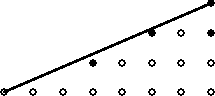
\includegraphics{pics/spin-377-pic-pics.pdf} \\
\caption{Generators in the $(\deg z, -ord_{P_i}(z))$ lattice}
\label{fig:377}
\end{figure}

Also note that $e_j' + 2k = 7 + 2k \nmid 2 = e_i - e_j'$ for all
$i, j \in J = \{2, 3\}$ such that $j \neq i$ and for all $k \geq
0$. Thus, $s_{\sigma, J}(i, k) = \emptyset$ for each $i \in J$.
Furthermore, $\deg \lfloor e_i \halfcan \rfloor = \deg \lfloor 9
\halfcan \rfloor = 2 \lfloor \frac{4 \cdot 9}{9} \rfloor + \lfloor
\frac{9}{3} \rfloor - 9 = 2$, so \ref{custom:Ad-iii} is satisfied and
$(\sigma, \sx', J)$ is admissible.

%Let $(-ord_{P_1}(x_j)$, $-ord_{P_2}(x_j)$, $-ord_{P_3}(x_j))$
%represent the pole orders of $x_i$ at each point. Then these generators
%must have pole orders $(1, 1, 1), (1, 2, 2), (2, 3, 2), (2, 2, 3)$
%respectively.

We can directly see that the relations are given in degrees $10$
and $14$. In particular, we have relations
\begin{align*}
	&a_1 x_{5, 1}^2 + a_2 x_{7, 2} x_{3, 1} + a_3 x_{7, 1} x_{3, 1} = 
	0 &\text{ in degree $10$} \\
	&b_1 x_{7, 2}^2 + b_2 x_{7, 2} x_{7, 1} + b_3 x_{7, 1}^2
	+ b_4 x_{5, 1} x_{3, 1}^3 = 0  &\text{ in degree $14$}
\end{align*}

\noindent
and note that $a_1$ and $b_1$ are both nonzero. If $a_1 = 0$, then we
have that
\[
	a_2 x_{7, 2} x_{3, 1} = -a_3 x_{7, 1} x_{3, 1}
\]

\noindent
However, $x_{7, 2} x_{3, 1}$ has pole orders $(3, 3, 4)$ and
$x_{7, 1} x_{3, 1}$ has pole orders $(3, 4, 3)$ so their
coefficients must be zero for this equality to hold. We have a
similar pole order consideration in forcing $b_1$ to be nonzero.

Let $I$ be the ideal generated by these relations in
$\Bk[x_{7, 2}, x_{7, 1}, x_{5, 1}, x_{3, 1}]$. Under grevlex with
$x_{3,1} \prec x_{5,1} \prec x_{7,1} \prec x_{7,2}$, the initial
ideal of $I$ is
\[
	\initial(I) = \langle x_{7, 2}^2, x_{5, 1}^2 \rangle
\]

\noindent
since $a_1$ and $b_1$ are nonzero.

To demonstrate that these two relations generate all 
relations, we show that $\dim_\Bk (R')_k = \dim_\Bk
(\Bk[x_{7, 2}, x_{7, 1}, x_{5, 1}, x_{3, 1}] / \initial(I))_k$ for 
all degrees $k \geq 0$. In particular, 

\begin{align*}
	\dim_\Bk \left(\Bk[x_{7, 2}, x_{7, 1}, x_{5, 1}, x_{3, 1}] / I\right)_k &=
	\dim_\Bk \left(\Bk[x_{7, 2}, x_{7, 1}, x_{5, 1}, x_{3, 1}]	/ \initial(I)\right)_k \\
	&= \dim_\Bk \left(\Bk[x_{7, 2}, x_{7, 1}, x_{5, 1}, x_{3, 1}] / \langle
	x_{7, 2}^2, x_{5, 1}^2 \rangle \right)_k
\end{align*}
\noindent
for all $k \geq 0$. But the fact $\dim_\Bk (R')_k = \dim_\Bk \left(\Bk[x_{7, 2},
x_{7, 1}, x_{5, 1}, x_{3, 1}] / \langle x_{7, 2}^2, x_{5, 1}^2
\rangle\right)_k$ can be checked by looking at the $\Bk$-basis at each degree
$k$.

Therefore, the canonical ring $R'$ has presentation $R' =
\Bk[x_{7, 2}, x_{7, 1}, x_{5, 1}, x_{3, 1}] / I$ with
initial ideal $\initial(I)$ generated by quadratics under grevlex
with $x_{3,1} \prec x_{5,1} \prec x_{7,1} \prec x_{7,2}$.
%These quadratics must also determine minimal generators for $I$ by
%Lemma ~\ref{lem:minimal_quadratic}.
Thus, $R'$ is generated up to degree $e = 7$ with relations up to
degree $2e = 14$, as desired.

%We can also see that $e_i > \deg z$ for any generator $z$ of $R'$
%since $e_i = 9 > e$ for all $i \in J$.
\end{example}

\begin{example}
\label{eg:base-1-33}
Let $(\sx',0 , \halfcan')$ be a log spin curve of genus $1$ with $\halfcan' = P - Q + \frac{1}{3}P_1 + \frac{1}{3}P_2$. In this example, we show
$$R_{\halfcan'} \cong \Bk[u, x_3, y_3, y_4]/(x_3 y_3- \alpha uy_4, y_4^2 - \beta x_3^2 u - \gamma y_3^2u)$$
and that $(\sx', \halfcan', \{1,2\})$ is admissible.

Let $u \in H^0(\sx,2\halfcan')$ be any nonzero element, let $x_3 \in H^0(\sx,3\halfcan')$ be an element with a pole at $P_1$ but not at $P_2$ and $y_3 \in H^0(\sx,3\halfcan')$ be an element with a pole at $P_2$ but not at $P_1$. Let $y_4 \in H^0(\sx,4\halfcan')$ be an element with a pole of order 1 at both $P_1$ and $P_2$. Note that $x_3$ and $y_3$ exist because the linear systems $3P - 3Q \sim P - Q$, $3P - 3Q + P_1$, and $3P - 3Q + P_1 + P_2$ are 0, 1, and 2 dimensional respectively.

Then, there exist constants $\alpha, \beta, \gamma \in \Bk$ so that 
$R_{\halfcan'} \cong \Bk[u, x, y_3, y_4]/(xy_3- \alpha uy_4, y_4^2 - \beta x^2 u - \gamma y^2u).$ The proof of this is fairly algorithmic: We may first use Riemann--Roch to compute the dimensions of $(R_{\halfcan'})_n$ over $\Bk$, then verify that these generators and relations produce the correct number of independent functions via an analysis of zero and pole order. The details are omitted as it is analogous to Example ~\ref{eg:base-0-377}.

We next check $(\sx', \halfcan', \{1,2\})$ is admissible. We have two generators $x_3$ and $y_3$ in degree 3 with a pole of order $1=\frac{3- 1}{2}$ by construction. Hence, \ref{custom:Ad-i} holds. We next check \ref{custom:Ad-ii} for the point $P_1$, as the case of $P_2$ is symmetric. Here, by construction
\[
\frac{-\ord_{P_1}(z)}{\ord(z)} = \begin{cases}
	0 &\text{ if }z \in \{u, y_3\}\\
	\frac{1}{4} &\text{ if }z = y_4
\end{cases}.
\]
Since $0, \frac{1}{4} < \frac{1}{3}$, \ref{custom:Ad-ii} holds.
Finally, to check \ref{custom:Ad-iii}, note that $\max_{k \geq 0}S_{\sigma,J}(i,k) = 0.$ Therefore, $\deg \lfloor 5L \rfloor  = 2 > 1 = (2 g - 1) + 0$.
\end{example}

\begin{example}
\label{eg:exception-1-5}
Let $(\sx', 0, L')$ be a log spin curve of genus 1 with $L' = P -
 Q + \frac{2}{5} P_1.$ Let $x_2 \in (R_L)_2$ be any nonzero element.
We obtain $\di x_2|_{P_1} = 0,$ since $2P - 2Q \sim 0$ and by Riemann
--Roch, $\dim_\Bk (P_L)_2 = 1.$ Let $y_3 \in (R_\halfcan)_3$ be any nonzero
element. We obtain $\di y_3|_{P_1} = - P_1,$ by Riemann Roch, since
if $y_3$ did not have a pole at $R$, we would obtain $y_3 \in H^0
(\sx,3P-3Q) \cong H^0(\sx, P - Q) \cong 0$ as $P \neq Q$. Finally,
let $y_5 \in (R_\halfcan)_5$ be an element with $y_5|_{P_1} = -P_1$. Then,
we claim there is some $\alpha \in \Bk$ so that

$$R_\halfcan \cong \Bk[x_2 , y_3, y_5]/(y_3^4 - \alpha x_2 y_5^2).$$

In order to show this is an isomorphism, one can use Riemann--Roch and pole order considerations at $P_1$ to check the above relation exists. One can then check that the generators and relation determine a ring $R$ so that for all $j \in \BZ,$ the $j$th graded component $(R)_j$ satisfies $\dim_\Bk (R)_j = \dim_\Bk R_\halfcan.$ Hence, $R \cong R_\halfcan$. The verification is analogous to Example ~\ref{eg:base-0-377} and is omitted.

Note that $(\sx', \halfcan', \{1\})$ is admissible, as can be checked in a fashion analogous to the verification in Example ~\ref{eg:base-1-33}.
\end{example}

\begin{rem}
\label{rem:base-0-377}
Examples ~\ref{eg:base-0-377}, \ref{eg:base-1-33}, and \ref{eg:exception-1-5} are used as inductive base cases in the genus 0, genus 1, and genus 1 sections respectively (see Tables ~\ref{table:g-0-base-cases} and ~\ref{table:g-1-base}).
\end{rem}

%%%%%%%%%%%%%%%%%%%%%%%%%%% Inductive lemmas %%%%%%%%%%%%%%%%%%%%%%%%%%%%%%%


\section{Inductive Lemmas}
\label{sec:induction}
First we present several lemmas which provide the inductive steps
for the proof of the main theorem (Theorem ~\ref{thm:main}). In
Subsection ~\ref{ssec:add-points} we prove three lemmas which
determine the generators and relations of $R_\halfcan = R_{\halfcan'
+ \frac{\alpha }{\beta}P}$ from those of $R_{\halfcan'}$, where
$\halfcan' \in \BQ \otimes \di X$ and $\frac{\alpha}{\beta} \in \BQ$. 
In Subsection ~\ref{ssec:raise-orders}, we prove an inductive lemma
allowing us to transfer information about the log spin canonical 
ring of a stacky curve to those of stacky curves with stabilizer
orders incremented by $2$ and fixed log divisor and stacky points.

%While Lemma ~\ref{lem:sat-1} may be applied in a fairly general 
%context, Lemma ~\ref{lem:raise-stacky-order} is more specific to 
%spin canonical divisors.

%However, before we can answer these general lemmas, it is useful
%to prove a nice result about minimal generation of ideals of
%relations.
%
%\todo{Include one of the following, if the first one, include a 
%remark for quotient}

%\begin{lem}
%\label{lem:minimal_quadratic}
%Suppose $k[x_1, \ldots, x_n]$ is a graded ring, not necessarily
%generated in degree 1, is equipped with a monomial ordering $\prec$.
 %Let $\phi:k[x_1, \ldots, x_n] \rightarrow B'$ be a map of graded
%rings with kernel $I'$, such that $I'$ is generated by elements $f_1,
%\ldots, f_j$, where $\initial(f_i) = x_i x_j,$ and no term of $f_i$
%is of the form $x_k$. Then, the elements $f_i$ determine minimal
%generators for $I$.
%\end{lem}
%\begin{proof}
%Regrade the ring $k[x_1, \ldots, x_n]$ so that all $x_i$ lie in
%degree 1. Then,
%\[
	%\phi : k[x_1, \ldots, x_n] \rightarrow B
%\]
%\noindent
%determines a map of rings, no longer necessarily graded. Consider
%the grlex monomial ordering $\prec$ on $k[x_1, \ldots, x_n]$.
%\todo{This ordering isn't quite right. 
%We need to preserve the ordering on quadratic terms}
%By
%assumption, the kernel $I$ is generated by elements whose initial
%terms have degree 2 and are all distinct. Therefore, $\dim_k (k[x_1,
%\ldots, x_n])_2 = \binom{n}{2} - j.$ This implies any set of
%generators for $I$ must have at least $j$ elements. Since $f_1,
%\ldots, f_j$ is such a set, it is minimal.
%\end{proof}
%
%\begin{rem}
%In particular, in the case of
%\[
	%\begin{tikzcd}
		%I\ar[hookrightarrow]{r}\ar[hookrightarrow]{d} & k[x_1, \ldots, x_n]
		%\ar[twoheadrightarrow]{r} \ar[hookrightarrow]{d} & B \ar[hookrightarrow]{d} \\
		%I' \ar[hookrightarrow]{r} & k[x_1, \ldots, x_n, y_1, \ldots, y_m] \ar[twoheadrightarrow]{r}& B'
	%\end{tikzcd}
%\]
%inducing
%\[
	%I/I'\hookrightarrow k[y_1, \ldots, y_m]\twoheadrightarrow B'/B
%\]
%\todo{how do we make this proof?}
%\end{rem}
%\begin{lem}
%\label{lem:minimal_quadratic}
%Suppose $k[x_1, \ldots, x_n]\hookrightarrow k[x_1, \ldots, x_n, y_1, \ldots, y_m]$ be graded ring, not necessarily
%generated in degree 1 that are equipped with monomial ordering $\prec$.
%Let $\phi: k[x_1, \ldots, x_n] \twoheadrightarrow B, \phi':k[x_1, \ldots, x_n, y_1, \ldots, y_m]\twoheadrightarrow B'$ be maps of graded
%rings with kernels $I \hookrightarrow I'$ such that the following diagram commutes:
%\[
	%\begin{tikzcd}
	%I\ar[hookrightarrow]{r}\ar[hookrightarrow]{d} & k[x_1, \ldots, x_n]\ar[twoheadrightarrow]{r} \ar[hookrightarrow]{d} & B \ar[hookrightarrow]{d}\\
	%I' \ar[hookrightarrow]{r} & k[x_1, \ldots, x_n, y_1, \ldots, y_m] \ar[twoheadrightarrow]{r}& B'
	%\end{tikzcd}
%\]
%Further suppose that $I'$ is generated over $I$ by elements $f_1,
%\ldots, f_j$ as a $k$-vector space, where $\initial(f_i) \in \{y_i x_j, y_i y_j\}$ and no monomial of $f_i$
%is of the form $y_i$. Then, the elements $f_i$ determine minimal
%generators for $I'$ over $I$.
%\end{lem}
%
%\begin{proof}
%Regrade the rings $k[x_1, \ldots, x_n], k[x_1, \ldots, x_n, y_1, \ldots, y_m]$ so that all $x_i$ and $y_j$ lie in
%degree 1. Then,
%\[
	%\phi : k[x_1, \ldots, x_n] \twoheadrightarrow B 
%\]
%\[
	%\phi': k[x_1, \ldots, x_n, y_1, \ldots, y_m] \twoheadrightarrow B'
%\]
%
%
%\noindent
%determines map of rings, no longer necessarily graded. 
%By assumption, $I'$ is generated over $I$ as a $k$-vector space by elements $f_1, \ldots, f_n$ whose initial terms have degree 2 and are linearly independent. By the theory of Gr\"{o}bner basis,
%\[
	%\dim_k(B'/B)_2=\dim_k(k[x_1, \ldots, x_n, y_1, \ldots, y_m]/k[x_1, \ldots, x_n])_2 - j
%\]
%so
%\[
	%\dim_k (I'/I)_2=j.
%\]
%This implies any set of
%generators for $I$ must have at least $j$ elements. Since $f_1,
%\ldots, f_j$ is such a set, it is minimal.
%\end{proof}
%
%\begin{rem}
%\label{rem:minimal_quadratic_trivial_case}
%It will be useful to use Lemma ~\ref{lem:minimal_quadratic} in the
%case $m= 0$, in which case we find explicitly that $f_1, \ldots, f_r$
%are $k$-minimal generators for $I'$ (over the trivial base vector
%space). 
%\end{rem}
%With this result, we will be able to show that the sets of generators of the ideal of relations in many of the following inductive arguments are minimal.


\ssec{Adding Points}
\label{ssec:add-points}
%In this section, we prove various inductive statements under the following setup:
%Let $\halfcan' \in \di \BQ \otimes X$ be $\BQ$-divisor of $X$ (and often a log spin canonical divisor of some $\sx'$), satisfying certain conditions about $\deg(\lfloor d \halfcan'\rfloor)$ for various values of $d \in\BN$ and certain saturation conditions. Let $\halfcan=\halfcan'+P$ for some $P$ possibly in the support of $\halfcan$.  Then we will explicitly describe elements that generate $R_\halfcan$ over $\halfcan$' and initial terms of relations that generate $\initial(I')$ over $\initial(I)$ (allowing the construction of a corresponding Gr\"{o}bner Basis). \todo{Aaron: What new ideas does this description add that wasn't already described in the previous paragraph? Also, in general it's a good idea to be specific about what the most important lemmas are in the section, although I also added this to the general description of section 3.}
%Before proving three lemmas that allow us to inductively add points to the support of a log spin canonical divisor
First, we give a criterion to determine if a set of monomials generates the initial ideal of relations of $\Bk[x_1, \ldots, x_m] \to R_D$.  This criterion will be used repeatedly to show that a given homogeneous ideal is in fact the ideal of relations.


\begin{lem}
\label{lem:relations_from_generators_induction} 
Suppose $\halfcan$, $\halfcan' \in \BQ$ $\otimes$ $\di X$ with $\halfcan=\halfcan'+\frac{\alpha}{\beta}P$, such that $R_{\halfcan'}$ generated by $x_1, \ldots, x_m$
and $R_{\halfcan}$ is minimally generated by $y_1, \ldots, y_n$ over 
$R_{\halfcan'}$.  Let $I'$ and $I$ be the ideals relations of $\phi':\Bk[x_1, \ldots, x_m]\to R_{\halfcan'}$ and $\phi:\Bk[x_1, \ldots, x_m, y_1, \ldots y_n]\to R_{\halfcan}$ respectively.
Suppose there are sets of monomials $S\subseteq R_\halfcan-R_{\halfcan'}$ and $T\subseteq R_\halfcan-(S\cup R_\halfcan')$, and a monomial ordering $\prec$ such 
\begin{enumerate}
\item $S$ forms a $\Bk$-basis for $R_\halfcan$ over $R_\halfcan'$
\item $T \succ S\succ \Bk[x_1, \ldots, x_n]$ {\rm(}meaning all monomials in $T$ are bigger than all monomials in $S$ which are bigger than all monomials in $\Bk[x_1, \ldots, x_n]${\rm)}
\item All monomials in $\Bk[x_1, \ldots, x_m, y_1, \ldots, y_n]$ lie in 
\begin{align*}
	S \; \cup\; \langle T\rangle \; \cup \; \initial(I') \Bk[x_1, \ldots, x_m, y_1, \ldots, y_n] \; \cup \; \Bk[x_1, \ldots, x_m]
\end{align*}
\end{enumerate}
Then,
\begin{align*}
	\initial(I) & = \initial(I') \Bk[x_1, \ldots, x_m, y_1, \ldots, y_n]
	+ \langle T \rangle.
\end{align*}
\end{lem}
\begin{proof}
First, notice that $I'\subseteq I$ so 
\[
	\initial(I)\supseteq \initial(I')\Bk[x_1, \ldots, x_m, y_1, \ldots, y_n].
\]

Now, let $f\in T$.  Since $S$ forms a $\Bk$-basis of $R_{\halfcan}$ over $R_{\halfcan'}$ by (1), we can write a relation $f - (\sum_{g\in S'} C_g g)-r=0$ for some finite subset $S'\subseteq S_{\deg(f)}$, $C_g\in \Bk$ for all $g\in S'$, and $r\in R_{\halfcan'}$.  This demonstrates that $\initial(I) \supseteq T$, and hence
\[
	\initial(I)\supseteq \initial(I')\Bk[x_1, \ldots, x_m, y_1, \ldots, y_n].
\]

To complete the proof, it suffices to show the reverse inclusion holds. By (2), any polynomial $G\in \Bk[x_1, \ldots, x_m, y_1, \ldots, y_n]$ with $\initial(\phi(G)) \in S$ cannot have a term in $T$.  Furthermore, since $S$ forms a $\Bk$-basis for $R_\halfcan$ over $R_{\halfcan'}$ by (1), and $\initial(\phi(G)) \in S,$ we obtain $\phi(G) \notin R_{\halfcan'} \subseteq R_\halfcan.$ Thus, $G=0$ is not a relation, so $f\not\in \initial(I)$.  Therefore, 
\[
	\initial(I)\subseteq R_\halfcan-S.
\]
In particular, there are no monomials in $I$ with initial terms in $S$.
Finally, note that
\[
	\initial(I) \cap \Bk[x_1, \ldots, x_m] = \initial(I').
\]

By (3), every monomial of $\Bk[x_1, \ldots, x_m, y_1, \ldots, y_n]$ is an element of either $S$, $\langle T\rangle$, or $\initial(I') \Bk[x_1, \ldots, x_m, y_1, \ldots, y_n].$ Therefore,
\begin{align*}
	\initial(I) & \subseteq \initial(I') \Bk[x_1, \ldots, x_m, y_1, \ldots, y_n] + \langle T \rangle.
\end{align*}
\end{proof}

To apply Lemma \ref{lem:relations_from_generators_induction}, we will need an appropriate monomial ordering.
The following definition provides the necessary ordering for the Lemma \ref{lem:sat-1}.
\begin{defn}
\label{defn:graded-p-lex}
Suppose $\halfcan$ is a divisor of $X$ such that $R_\halfcan$ is generated by $x_1, \ldots x_m$.  Then we have a map $\phi: \Bk[z_1, \ldots z_m] \rightarrow R_\halfcan, z_i\mapsto x_i$. If $P$ is a point in $X$, then $\phi$ defines a graded-$P$-lexicographic order (shortened to {\bf{graded $P$-lex}}) on $\Bk[z_1, \ldots, z_m]$ as follows.
If $f=\prod_{i=1}^m {z_i}^{q_i}$ and $g=\prod_{i=1}^m {z_i}^{r_i}$ with $f \neq g,$ then $f\prec g$ if one of the following holds:
\begin{enumerate}
\item $\deg(f) < \deg(g)$
\item $\deg(f) = \deg(g)$ and $-\ord_P(f) < -\ord_P(g)$
\item $\deg(f) = \deg(g)$, $-\ord_P(f) = -\ord_P(g)$, and $q_i > r_i$ for the largest $i$ such that $q_i\ne r_i$
\end{enumerate}
\end{defn}

\begin{rem}\label{rem:graded-P-lex-independent-of-line-bundle}
Observe that Definition \ref{defn:graded-p-lex} remains the same if we replace $-\ord_P$ with $-\ord_P^{L'}$ for any divisor $\halfcan'$ of $X$.
\end{rem}

\noindent One can easily verify graded $P$-lex is a monomial ordering in the sense defined in Cox--Little--O'Shea \cite[Chapter 2, $\mathsection$ 2, Definition 1]{cls:ideals-varieties-algorithms}.

We are almost ready to state Lemma ~\ref{lem:sat-1}, which will yield an inductive procedure for determining the generators and relations of $R_D$, where $D \in \di \BP^1$ is an effective $
\BQ$-divisor. Whereas O'Dorney considers arbitrary $\BQ$-divisors in $Div(\mathbb{P}^1)$ \cite[Theorem 8]{dorney:canonical}, we restrict attention to effective divisors and in Lemma ~\ref{lem:sat-1} we are able to obtain much tighter bounds.  Moreover, Lemma ~\ref{lem:sat-1} also extends to curves of genus $g > 0$. Before stating Lemma ~\ref{lem:sat-1}, we recall some notation from O'Dorney \cite{dorney:canonical}.

\begin{defn}\label{den:lower-approximation}
If $\frac{\alpha}{\beta}\in \BQ$, then $\frac{c}{k}$ (written in reduced form with $c \in \BN, k \in \BN$) is a {\bf{best lower approximation}} to $\frac{\alpha}{\beta}$ if there does not exist any $\frac{c'}{k'}\in \mathbf{Q}$ with $0<k'<k$ and $\frac{c}{k}\le \frac{c'}{k'}$. 
\end{defn}
Moreover, if $\frac{\alpha}{\beta}\ge 0$, then the non-negative best lower approximations of $\frac{\alpha}{\beta}$ form a finite sequence
\[
	0=\frac{c_0}{k_0} < \frac{c_1}{k_1} < \ldots < \frac{c_r}{k_r} = \frac{\alpha}{\beta}.
\]
Figure \ref{fig:s14/5-lattice} gives a pictorial representation of the positive best lower approximations of $\frac{\alpha}{\beta}=\frac{14}{5}$.

\begin{figure}
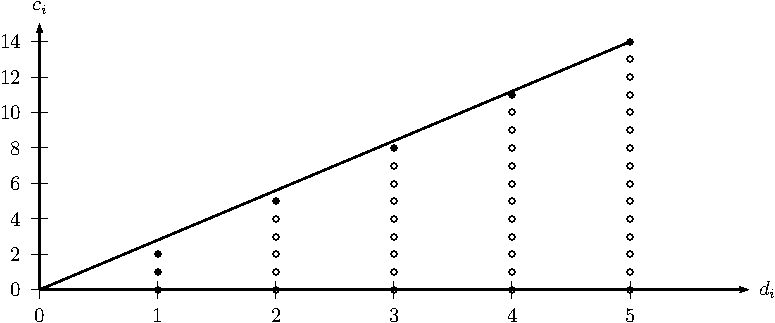
\includegraphics{pics/spin-lower-approximations-pic-pics.pdf}
\caption{This figure shows each non-negative best lower approximation of $\frac{14}{5}.$ Each ``$\bullet$'' denotes a best lower approximation and each ``$\circ$'' denotes a lattice point below $5y=14x$ which is not a best lower approximation.  Note that the non-negative best lower approximations generate the monoid of lattice points in the first quadrant satisfying  $5y \le 14x$, with the operation $(a_1, b_1)(a_2, b_2)\mapsto (a_1 + a_2, b_1 + b_2)$ .}\label{fig:s14/5-lattice}
\end{figure}

We next prove the first of three lemmas used to inductively add points.

\begin{lem}
\label{lem:sat-1}
Let $X$ be a genus $g$ curve and $\halfcan' \in \BQ \otimes \di X$
satisfying $h^0(X, \lfloor{\halfcan'}\rfloor)\ge 1$. Suppose $P$ is not a base-point of $k\halfcan'$ for all $k \in \BN$, meaning we can choose generators $u, x_1, \ldots, x_m$ of $R_{\halfcan'}$ in degree at most $\tau$ for some $\tau\in \BN$, with $\deg u = 1$, $\ord_P^{\halfcan'}(x_i)=0$ for all $1 \leq i \leq m$, and $\ord_P^{\halfcan'}(u) = 0$.  Suppose $\halfcan = \halfcan' + \frac{\alpha}{\beta} P$
for some $\alpha, \beta \in \BN$ such that
\begin{align}
\label{eqn:deg1-sat-ind}
	h^0(X, \lfloor k \halfcan \rfloor) &= h^0(X, \lfloor k \halfcan'
	\rfloor) + \left\lfloor k \frac{\alpha} {\beta} \right \rfloor &&\text{ for all } k \in \mathbb{
	N}.
\end{align}
Let
\[
	0 < \frac{c_1}{k_1} < \ldots < \frac{c_n}{k_n} = \frac{\alpha}{\beta}
\]
be the positive best lower approximations of $\frac{\alpha}{\beta}$.
Then,

\begin{enumerate}
\item[(a)] $R_{\halfcan}$ is generated over $R_{\halfcan'}$ by 
	elements $y_1, \ldots, y_n$ such that $\deg(y_i) = k_i$ and $-\ord_P
	^{L'}(y_i) = c_i$.

\item[(b)] Choose an ordering $\prec$ on $\Bk[u, x_1, \ldots, x_m]$ such that
	\[
		\ord_u(f) < \ord_u(h) \implies f\prec h.
	\]
	Equip $\Bk[y_1, \ldots, y_n]$ with graded $P$-lex, as defined in
	Definition ~\ref{defn:graded-p-lex} and $\Bk[y_1, \ldots, y_n] \otimes \Bk[u, x_1, \ldots, x_m]$ with block order.
	If $I'$ and $I$ are the ideals of relations of $\Bk[u, x_1, \ldots, x_m]
	\to R_{\halfcan'}$ and $\Bk[u, x_1, \ldots, x_m, y_1, \ldots, y_n]
	\to R_{\halfcan}$ respectively, then

	\begin{align*}
		\initial(I) &= \initial(I') \Bk[u, x_1, \ldots, x_m, y_1, \ldots, y_n] 
											 + \langle U_i: 1 \le i \le n-1 \rangle
											 + \langle V \rangle, \\
	\end{align*}
	where $V = \{x_i y_j: 1 \le i \le m, 1 \le j \le n\}$ and $U_i$ is
	the set of monomials of the form $\prod_{j = 1}^{i} y_j^{a_j}$ with
	$a_j \in \BN_{\ge 0}$ such that
	\begin{enumerate}
		\item[\customlabel{custom:sat-1-*}{(U-1)}] $\sum_{j = 1}^i a_j c_j \ge c_{i+1}$, \\
		\item[\customlabel{custom:sat-1-**}{(U-2)}] there does not exist $(b_1, \ldots b_i) \ne (a_1,
			\ldots a_i)$ with all $b_j \le a_j$ and $\sum_{j = 1}^i b_j
			c_j \ge	c_{i + 1}$, \\
		\item[\customlabel{custom:sat-1-***}{(U-3)}] there does not
			exist $r<i$ such that $\sum_{j=1}^r a_j c_j> c_{r + 1}$.
	\end{enumerate}

\item[(c)] In particular, $R_\halfcan$ is generated over $R_\halfcan'$
	in degrees at most $\beta$ with $I$ generated over $I'$ in
	degrees at most $\max(2 \beta, \beta + \tau)$ (where $\tau = \max(1,
	\max_{1 \leq i \leq m}(\deg(x_i)))$).
\end{enumerate}
\end{lem}

\begin{proof}
{\bf Part (a):}
By
Equation ~\ref{eqn:deg1-sat-ind}, for any $k
\in \BN$ such that $\lfloor k \frac{ \alpha}{\beta} \rfloor > 0$,

\[
	h^0 (X, k \halfcan ) = h^0(X, k \halfcan') + \lfloor k \frac{\alpha}{\beta}\rfloor.
\]

\noindent
Thus, there exist rational sections $t_i$ of $\sco(\lfloor k \halfcan \rfloor)$ with $\ord_P^{L'}(t_i) = i$
for any $i \in \{0, \ldots, \lfloor d \frac{\alpha}{
\beta} \rfloor \}$. We will the use positive best lower approximations to
construct the generators $y_1, \ldots, y_n$ as described in the lemma's statement.

Let 
\[
	0 < \frac{c_1}{d_1} < \ldots < \frac{c_n}{d_n} = \frac{\alpha}{
	\beta}
\]

\noindent
be the positive best lower approximations of $\frac{
\alpha}{\beta}$. 
%Note that the elements $t_1, \ldots, t_{\lfloor d_i \frac{\alpha}{\beta}\rfloor}$ in $(R_{\halfcan})_{d_i}$ with $\ord_P^{\halfcan'}(t_i) = i$ are linearly independent over $(R_{\halfcan'})_d$. Hence, by a dimension count, these sections form a $k$-basis for
%$(R_{\halfcan})_d$ over $(R_{\halfcan'})_d$.\todo{take out two sentences}
%For any $1\le i < j \le n$, we have $\frac{c_i}{d_i} < \frac{c_j}{d_j}$.  
Choose a positive best lower approximation $\frac{c_i}{k_i}$.  Choose $z_1, \ldots, z_r \in R_\halfcan$ so that $\sum_{j=1}^r \deg(z_j) = k_i$ and $\deg(z_j)<k_i$ for all $j\in \{1, \ldots r\}$. Observe that $\frac{-\ord_P^{\halfcan'}(z_j)}{\deg(z_j)}< \frac{\alpha}{\beta}$, for each $j$.  Hence, for each $j$, 
\[
	\frac{-\ord_P^{\halfcan'}(z_j)}{\deg(z_j)} < \frac{c_i}{k_i},
\]
so the mediant inequality tells us
\[
	\frac{\sum_{j=1}^n -\ord^{\halfcan'}_P(z_j)}{\sum_{j=1}^n z_j } < \frac{c_i}{k_i}.
\]
Multiplying through by $k_i$ gives
\[
	-\ord^{\halfcan'}_P \left(\prod_{j=1}^n z_j \right) = \sum_{j=1}^n -\ord^{\halfcan'}_P(z_j) < c_i .
\]

\noindent
Thus, the elements of $(R_{\halfcan})_{k_i}$ with pole order $c_i$ at $P$ are not generated by 
lower degrees. 
Choose some $y_i \in(R_{
\halfcan})_{k_i}$ with $-\ord_{P}^{L'}(y_i)=c_i$.

Suppose $c,k \in \BN$ so that $k \le \beta$,  $\frac{c}{k} < \frac{\alpha}{
\beta},$ and $\frac{c}{k}$ is not a best lower approximation of $\frac{\alpha}{\beta}$. Choose a
best lower approximation $\frac{c_i}{k_i}$ with $c_i$ maximal such that $k_i< k$.  This implies $\frac{c_i}{k_i}\ge \frac{c}{k},$ so 
%  The argument goes $c_i d \ge c k_i$
% implies c_i \frac{k}{k_i} \ge c
% implies c_i + \frac{k-k_i}{k_i}c_i \ge c
% \implies c_i (k-k_i) \frac{c_i}{k_i}\ge c
% so since everything is an integer $c_i +\lfloor (k - k_i) \frac{c_i}{k_i}\rfloor \ge c$
% \implies the equation below:
\[
	\frac{c-c_i}{k-k_i}\le \frac{\alpha}{\beta}
\]
which implies
\begin{equation}\label{eqn:c-from-lower-terms}
	c_i +\left\lfloor (k-k_i) \frac{\alpha}{\beta} \right\rfloor \ge c.
\end{equation}

Using Equation ~\ref{eqn:c-from-lower-terms}, we recursively define a $\Bk$-basis for $R_\halfcan$ over $R_{\halfcan'}$. Define 
\[
	S_0 = \{u^l : l \in \BN_{\ge 0}\}
\]
and for each $i \in \BN$, suppose $c_j$ is the maximal element among of $c_1, \ldots c_n$ such that $c_j \le i.$ Note that such a $c_j$ exists because $1=c_1\le i.$ Define
\[
	S_i = y_j \cdot S_{i-j}.
\]
Since each $y_j$ has pole order $c_j$, this recursive construction ensures that 
\[
	z\in S_i \implies -\ord_P^{\halfcan'}(z)=i.
\]
Then define 
\begin{equation}\label{eqn:sat-1-defining-S}
	S = \bigcup_{i=1}^{\infty} S_i.  
\end{equation}
Note that $S_0$ is not part of this union and in fact $S\cap S_0 = \emptyset$ by pole order considerations.

By equation \ref{eqn:deg1-sat-ind} for $k \in \BN$,
\[
	h^0(X, \lfloor k \halfcan \rfloor) = h^0(X, \lfloor k \halfcan'
		\rfloor) + \left\lfloor k \frac{\alpha} {\beta} \right \rfloor,
\] 
so $S$ contains elements in degree $k \in \BN$ with each pole order in $\{1 \ldots, \lfloor k\frac{\alpha}{\beta}\rfloor\}$.  Thus, by dimension counting, $S$ forms a $\Bk$-basis for $R_\halfcan$ over $R_{\halfcan'}$, and we have proven part (a).

{\bf Part (b):}
Let $S$ be as defined in Equation \ref{eqn:sat-1-defining-S}, define $U_i$ and $V$ as in the lemma's statement, and set
\[
	T = \left(\bigcup_{i=1}^{n-1} U_i \right) \cup V.
\]

We check that $S$, $T$, and $\prec$ meet the hypothesis of Lemma \ref{lem:relations_from_generators_induction}.  In part (a), we showed that $S$ forms a $\Bk$-basis for $R_\halfcan$ over $R_{\halfcan'}$ giving condition (1) of Lemma ~\ref{lem:relations_from_generators_induction}.  Our choice of monomial order in $\Bk[y_1, \ldots, y_n]$ and block order for $\Bk[y_1, \ldots, y_n]\otimes \Bk[u, x_1, \ldots, x_m, y_1, \ldots, y_n]$ implies that $T\succ S\succ \Bk[u, x_1, \ldots, x_m]$, giving condition (2) of Lemma \ref{lem:relations_from_generators_induction}.  

It only remains to check condition (3) of Lemma ~\ref{lem:relations_from_generators_induction}. To do this, suppose $f\in \Bk[u, x_1, \ldots, x_m, y_1, \ldots, y_n]$ is a monomial not contained in $\Bk[u, x_1, \ldots, x_m]$, meaning there is some $j$ such that $y_j|f$.  Further suppose $f\not\in \langle V \rangle$, meaning that for each $i\in \{1, \ldots m\}$, $x_iy_j \nmid f$. Since $y_j \mid f$ but $x_iy_j \nmid f$, we obtain $x_i\nmid f$.  Therefore, $f\in \Bk[u, y_1, \ldots, y_n]$.  We note that $S$ generates $y_j \cdot (\Bk[u,y_1, \ldots, y_n])$ as a $\Bk$-algebra.  That is, all monomials of $\Bk[u, x_1, \ldots, x_m, y_1, \ldots, y_n]$ are contained in
\[
	\Bk[u, x_1, \ldots, x_m] \cup V \cup \left(\bigcup_{i=1}^n y_i \cdot \Bk[u, y_1, \ldots, y_n]\right). 
\]
Notice that $S$ generates the ideal $(y_1, \ldots, y_n)$ considered as an ideal of the subring $\Bk[u, y_1, \ldots, y_n]$.  If $f\in S$, then $f=u^b \prod_{j=1}^n {y_j}^{a_j}$. Let $\halfcan$ be maximal such that $a_l\ne 0$.
Fix $i \in \{1, \ldots, n\}$. If $y_i \cdot f \notin S$, define
\[
b_j = \begin{cases}
	a_j &\text{ if } j \neq i\\
	a_j + 1 &\text{ if } j=i.
\end{cases}
\]

\noindent
Then, there is some $h \in \BN$ such that $i \le h \le \max(i, l)$ satisfying $\prod_{j = 1}^h y_j^{b_j}\not\in S$, 
and for all $r<h$ we have $\prod_{j=1}^r {y_j}^{b_j}\in S$.  
Choose some tuple $(\gamma_1, \ldots, \gamma_n)$ which is minimal, in the sense that we cannot decrease any $\gamma_j$ 
and have the following still satisfied: each $\gamma_j\le b_j$ 
and $\prod_{j=1}^h {y_j}^{\gamma_j}\not\in S.$ Our recursive definition of 
$S$ and the fact that $\prod_{j=1}^r {y_j}^{b_j}\in S$ implies that for each $1\le r< h$, we have $\prod_{j=1}^r {y_j}^{\gamma_j}\in S$.

We now check that $\prod_{j=1}^h y_j^{\gamma_j}\in U_{h}$, by checking conditions \ref{custom:sat-1-*}, \ref{custom:sat-1-**}, and \ref{custom:sat-1-***}.  
Notice that if $r\le n$, $\omega_1, \ldots \omega_r\in \mathbb{Z}_{\ge 0}$, and $\prod_{j=1}^r y_j^{\omega_j}\in S$, then our definition of $S$ implies $y_r\prod_{j=1}^r y_j^{\omega_j}\in S$ if and only if $c_r$ is maximal among $c_1, \ldots c_n$ not greater than than $c_r + \sum_{j=1}^r c_j \omega_j$.
Therefore, since $\prod_{j=1}^{h-1} y_j^{b_j}\in S$ but $\prod_{j=1}^h y_j^{b_j}\not\in S$, $c_h$ must not be maximal (among $c_1, \ldots, c_n$) such that $c_h \le \sum_{j=1}^h b_jc_j$, which means $c_{h+1}\le \sum_{j=1}^h b_jc_j$.  Therefore $\sum_{j=1}^h {y_j}^{\gamma_j}$ satisfies \ref{custom:sat-1-*}.  

Next, suppose we choose $\omega_1, \ldots, \omega_h$ such that $\omega_j\le \gamma_j$ for all $j$ and $\omega_l \le \gamma_l$ for some $l$.  Then, for all $r< h$ we have $\prod_{j=1}^r {y_j}^{\gamma_j}\in S$, implying that for all $r< h$ we also have $\prod_{j=1}^r {y_j}^{\omega_j}\in S$.  Furthermore, since $(\gamma_1, \ldots, \gamma_h)$ was chosen to be minimal to satisfy the previous condition and that $\prod_{j=1}^h {y_j}^{\gamma_j}\not\in S$, we have $\prod_{j=1}^h {y_j}^{\omega_j}\in S$.  Therefore, $c_h$ is minimal among $c_1, \ldots c_n$ that is not greater than $\sum_{j=1}^h c_j \omega_j$, so in particular $\sum_{j=1}^h c_j\omega_j < c_{h+1}$; therefore, $\prod_{j=1}^h {y_j}^{\gamma_j}$ satisfies condition \ref{custom:sat-1-**}.  
Since for each $r<h$, we have $\prod_{j=1}^r y_{j}^{\gamma_j}\in S$ meaning that $\sum_{j=1}^r \gamma_j c_j < c_{r+1}$, condition \ref{custom:sat-1-***} holds for $\prod_{j=1}^h y_j^{\gamma_j}$.  
Thus $\prod_{j=1}^h y_j^{\gamma_j}\in U_{h}$.

Since the ideal in $\Bk[u, y_1, \ldots, y_n]$ generated by is $S$ is $(y_1, \ldots, y_n) \cdot \Bk[u, y_1, \ldots, y_n]$ and $\bigcup_{i=1}^{n-1} U_i$ generates every monomial in $\bigcup_{i=1}^n y_i \cdot \Bk[u, y_1, \ldots, y_n]-S$, we have shown that all monomials of $\Bk[u, x_1, \ldots, x_m, y_1, \ldots, y_n]$ are contained in
\begin{align*}
				& \Bk[u, x_1, \ldots, x_m] \cup \langle V \rangle \cup S \cup \left\langle \bigcup_{i=1}^{n-1} U_i \right\rangle \\
	\subseteq \; 	& S \cup \langle T\rangle \cup \initial(I') \Bk[u, x_1, \ldots, x_m, y_1, \ldots, y_n] \; \cup \; \Bk[u, x_1, \ldots, x_m].
\end{align*}
This shows condition (3) of Lemma ~\ref{lem:relations_from_generators_induction} holds.  Thus, the conditions of 
Lemma ~\ref{lem:relations_from_generators_induction} are met. Finally, Lemma ~\ref{lem:relations_from_generators_induction} implies part (b).

{\bf Part (c):}
Finally, (c) of this lemma follows immediately by looking at the constructions of parts (a) and (b).  






%Thus, for a general $d$ (not necessarily less than $\beta$), if $\frac{c}{d} \le
%\frac{\alpha}{\beta}$ is not a best lower approximation than we can
%construct an element in degree $d$ with pole degree $c$ by either $y
%_n^a y_i u^b$, $y_n^a zy_iu^b$ or $y_n^a z u^b$ satisfying the
%same conditions.  This forms a $k$-basis for $R_{\halfcan}$ over $R_{\halfcan'}$ and $y_1, \ldots, y_n$ generate $R_{\halfcan}$ over $R_{\halfcan'}$.  In particular, we see this generating set corresponds to the best positive approximations of $\frac{\alpha}{\beta}$.
%
%Choose $x_i\in \{x_1, \ldots, x_m\}$ and $y_j\in \{y_1, \ldots, y_n\}$.  Choose an element of the form $y_n^a y_l u^b$ and $y_n^a y_l y_{l'} u^b$ as described in the previous paragraph, in degree with $d_l= 1$ and if 
%$d_{l'}= 1$ then $c_{l'} = \lfloor \frac{\alpha}{\beta} \rfloor$. Specifically, we can 
%successively subtract some $\gamma_l y_l u^{b_l}$, $\gamma_l y_l z_l u^{b_l}$, or $
%\gamma_l z_l$ with $y_l, z_l, b_l$ satisfying the same conditions as above and $\gamma_l
%\in k$ the element ensuring that the difference decreases in pole degree at $P$ by 1. For 
%convenience, we can combine these into the case $\gamma_l (y_l)^{s_l}(z_l)^{a_l}u^{b_l}$ 
%with $(s_l,a_l)\in \{(1,0),(1,1),(0,1)\}$. In the cases when $\frac{\alpha}{\beta}<1$ so $z_l$ 
%is not well-defined, just pick an arbitrary element of $R_{\halfcan'}$ for $z_l$ ensuring that the 
%expression still makes sense; in such cases we will always choose $a_l= 0$ so this choice 
%is irrelevant, and only makes writing out cases more convenient. Therefore, we can write
%\[
	%x_i y_j - \sum_{l} (y_l)^{s_l} (z_l)^{a_l} u^{b_l}\in R_D
%\]
%
%\noindent
%giving us a non-trivial relation with leading term $x_i y_j$. \todo{Explicitly state ordering at 
%the beginning}
%
%Similarly, suppose $y_i, y_j\in \{y_1, \ldots , y_{n - 1}\}$ with $1
%< d_i$ and $j \ge i$ (that is, so $y_i y_j$ does not appear as a
%basis element of the form described above: $y_n^0 y_j y_i u^0$). 
%Choose the maximal $\halfcan$ such that $c_h \le c_i + c_j$; since $1 < d_i
%\le d_j$, $(c_i + c_j) - c_j>\lfloor \frac{\alpha}{\beta}\rfloor$
%so $c_{j + 1} < c_i + c_j$ meaning $c_h \ge c_{j + 1} > c_j$.
%Furthermore, $c_i + c_j - c_h < \lfloor \frac{\alpha}{\beta} \rfloor
%$ so either $c_h = c_i + c_j$ or there is some $h'$ such that $c_{h'}
%= c_i + c_j - c_l$ and $d_{h'}= 1$. Since $\frac{c_h}{d_h}$ is a
%best lower approximation of $\frac{\alpha}{\beta}$ with denominator
%larger than those of $\frac{c_i}{d_i}$ and $\frac{c_j}{d_j}$, we
%know that since $c_h\le c_i + c_j$ we must have $d_h < d_i + d_j$. 
%Thus in the case with a $y_{l'}$ term we have $d_h + d_{h'} = d_h +
%1 \le d_i + d_j$. That is to say, by choosing $b - d_i + d_j - a d_
%h - 1$ we find (where $a \in \{0,1\}$ corresponding to if a $y_{h'}$
%appears) that $y_h (y_h')^a u^b$ and $y_i y_j$ both lie in degree
%$d_i + d_j$ with pole order $c_i + c_j$ at $P$. From here we can
%follow a similar technique as in the previous paragraph to cancel
%out poles of $y_i y_j$ at $P $ to find
%\[
	%y_i y_j -\gamma_h (y_h)^{s_h}(z_{h})^{a_h}u^{b_h} -\sum_l (y_l)^{s_l} (z_{l})^{a_l}
	%u^{b_l}\in R_D
%\]
%
%\noindent
%implying a relation with initial term $y_i y_j$. 
%
%Next, suppose $y_i, y_j \in \{y_1, \ldots , y_{n - 1}\}$ such that
%$i \le j$, $d_j = d_i = 1$, and $d_{j + 1} = 1$ (i.e.,~ $c_i, c_j \le
%\lfloor \frac{\alpha}{\beta} - 1 \rfloor$). If $i > 1$ and then $y_
%{j + 1} y_{i - 1}$ lies in the same degree as $y_i y_j$ (degree 2)
%with the same pole order; following the same method as the previous
%two paragraphs we find
%\[
	%y_i y_j - \gamma y_{i - 1} y_{j + 1} - \sum_{l} (y_l)^{s_l} (z_l)^{a_l}u^{b_l}\in R_D.
%\]
%
%\noindent
%Similarly if $i = 1$, then we get the same result using
%\[
	%y_i y_j - \gamma u y_{j + 1} - \sum_l y_l u^{b_l} \in R_D.
%\]
%
%\noindent
%In both cases we deduce that $y_i y_j$ is an initial term of some relation.
%
%
%Finally, we examine the case (for $\alpha \ge \beta$) of $(y_i)^{i +
%1}$ when $i = \lfloor \frac{\alpha}{\beta}\rfloor$. If $\beta = 1$,
%then there are no relations with initial term a power of $y_i$
%and we are immediately done. Otherwise, assuming $\beta \ne 1$, we
%note that $c_i d_{i + 1} = c_{i + 1} d_i + 1 = c_{i + 1} + 1$. \todo
%{reference to Evan's paper where he proves this} Therefore, if $i >
 %1$ then $c_i^{d_{i + 1} + 1}$ and $c_{i - 1} c_{i + 1}$ both lie
%in the $d_{i + 1} + 1$ degree with pole order $c_{i + 1} + 1$.
%Following a similar technique to the previous paragraphs we find
%\[
	%(y_i)^{c_{i + 1} + 1} - y_{i + 1} y_{i - 1} - \sum_l (y_l)^{s_l}(z_l)^{a_l} u^{b_l}.
%\]
%
%\noindent
%Similarly if $i = 1$ then
%\[
	%(y_i)^{c_{i + 1} + 1} - y_{i + 1}u - \sum_l (z_l)^{a_l} u^{b_l}.
%\]
%
%\noindent
%In each case we demonstrate $(y_i)^{c_{i + 1} + 1}$ as the initial term of a relation. 
%
%Let $J$ be the ideal of $k[u, x_1, \ldots, x_m, y_1, \ldots, y_n]$
%generated by the initial terms described in the previous paragraphs
%together with $\initial(I) k[u, x_1, \ldots, x_m, y_1, \ldots, y_n]$.
%
%We show that $J$ is in fact all of the initial ideal. Suppose
%$f$ is a non-constant monomial that does not lie within $J$.
%Further suppose $f$ does not lie in $k[u, x_1, \ldots, x_m]$. Then
%there is some $y_i \mid f$. Since $f \not\in j$, we cannot have
%some $x_j \mid f$ or else we would have $y_i x_j \mid f$
%contradicting $f \not\in J$. Furthermore, if $y_l \mid f$ for $l <
%i$, then we must have $d_l = 1$ or else $y_l y_i$ is an initial
%element of a relation and divides $f$. If $d_i = 1$ as well, then
%we must have $c_i = \lfloor \frac{\alpha} {\beta} \rfloor$, or else
%$y_i y_l \in I$; finally we can not have $(y_{\lfloor \frac{\alpha}{
%\beta} \rfloor})^{d_{\lfloor \frac{\alpha}{\beta} \rfloor + 1} + 1} \mid
%f$. We observe that the remaining elements are precisely those of
%the form $y_n^a y_i u^b$, $y_n^a z y_i u^b$, and $y_n^a z u^b$
%which are the elements of our chosen $k$-basis for $k[u, x_1, \ldots
%, x_m, y_1, \ldots, y_n]/I'$ over $k[u, x_1, \ldots, x_m]/I$.
%Therefore, by dimension counting (in each degree), we see that $J$
%is the initial ideal of $I$. 


%Furthermore, since our choice of $y_i
%$'s was generic, this is in fact the generic initial ideal.

%In the case when all $\frac{\alpha}{\beta}\le 1$, Lemma
%~\ref{lem:minimal_quadratic} immediately tells us that the Gr\"{o}bner
%basis defined above is minimal.
%\todo{What about $\frac{\alpha}{\beta} > 1$?}
\end{proof}

\begin{rem}\label{rem:quad-gen}
If $\frac{\alpha}{\beta}=\frac{e_i-1}{2 e_i}$ for some odd $e_i \in \BN_{\geq 3}$, then $T,$ as defined in the beginning of the proof of (b) in Lemma \ref{lem:sat-1} consists only of terms of the form $x_i y_j$ and $y_i y_j$, which are quadratic in the generators.
\end{rem}


\begin{rem}\label{rem:sat-1-gen-lem-generic}
The generators in Lemma \ref{lem:sat-1} are generic if $\frac{\alpha}{\beta}\le 1$ (since there is at most one positive best lower approximation $\frac{c_i}{k_i}$ with $k_i=1$).  When $\frac{\alpha}{\beta}>1$, the choice of generators in degrees great than 1 is generic; furthermore, we can make the choice in degree 1 generic by choosing $\lfloor \frac{\alpha}{\beta}\rfloor$ linearly independent elements in degree 1 with pole at $P$ of order $\lfloor \frac{\alpha}{\beta}\rfloor$ rather than elements with poles of order $1, \ldots, \lfloor \frac{\alpha}{\beta}\rfloor$; this requires minor complications in the construction of generators of the ideal of relations.
\end{rem}

We now restrict our attention to log canonical rings of stacky curves.  Lemma \ref{lem:sat-1} accounts for many of the induction cases when the spin canonical ring is saturated in degree 1, as defined in Definition ~\ref{defn:sat}.  We complement Lemma ~\ref{lem:sat-1} with the following two lemmas that allow us to inductively add points, under certain conditions when the spin canonical ring is saturated in degree two or three.

\begin{lem}
\label{lem:sat-2}
Let $(\sx, \Delta, \halfcan)$ and $(\sx', \Delta, \halfcan')$ be log spin curves with the same coarse space $X = X'$ having signatures $(g; e_1, \ldots, e_r; \delta)$ and $(g, e_1, \ldots, e_{r- 1}, \delta)$, where $e_r=3$.  Suppose $g > 0,$ and, if $g = 1,$ then $\deg 3\halfcan' \geq 2.$ Then, by Riemann-Roch $\sat(Eff(L'))\le 2$.
Furthermore, let $R_{\halfcan'} = \Bk[x_2, x_3
, x_5, \ldots, x_m]/I'$ and let $\halfcan = \halfcan' + \frac{1}{
3}P$, where $P\in X$ is a base point of $\halfcan'$ (which includes the case when $H^0(X, \lfloor \halfcan'\rfloor) = 0$).
Suppose for $i \in \{2, 3\}$, we generically choose $x_i$ satisfying $\deg x_i = i$ and $\ord_P^{\halfcan'}(x_i)= 0$. Choose an ordering on $\Bk[x_2, \ldots, x_m]$ that satisfies
\begin{align*}
	\ord_{x_2}(f) < \ord_{x_2}(h) \implies f \prec h.
\end{align*}

\noindent
Then, the following statements hold.

\begin{enumerate}
	\item[(a)] General elements  $y_i \in H^0(\sx,iL)$ for $i \in
		\{3, 4\}$ satisfy $-\ord_P^{\halfcan'}(y_i) = 1$ and any such choice of elements
		$y_3, y_4,$ minimally generate $R_\halfcan$ over $R_{\halfcan'}$.
	\item[(b)] Equip $\Bk[y_3, y_4]$ with $grevlex$ so that $y_3 \prec 
		y_4$
		and equip the ring $\Bk[y_3, y_4] \otimes \Bk[x_2, \ldots, x_m]$ with block 
		order. Then,
		\begin{align*}
			\initial(I) &= \initial(I')\Bk[x, y_3, y_4]+\langle y_4 x_j \mid 2 \leq j \leq m \rangle +\langle y_4^2 \rangle.
		\end{align*}
	%\item[(c)] Any set of minimal generators for $I'$ together with 
		%any set of relations with leading terms as in (b) minimally 
		%generate $I$.
\end{enumerate}
\end{lem}

\begin{proof}
First, note that when genus is at least we shall show the assumptions on $g$ imply $H^0(\sx, 3 \halfcan), H^0(\sx, 4 \halfcan)$ are both basepoint-free: If $g \geq 2$ then $\deg 3 \halfcan > 2g - 1$ 
and $\deg 4 \halfcan > 2g - 1$, so $H^0(\sx, 3 \halfcan)$ and $H^0(\sx, 4 \halfcan)$ are base point free. If $g = 1$, we assume $\deg 3 \halfcan \geq 2 > 2g - 1$, so we also have $\deg 4 \halfcan \geq 2 > 2g - 1,$ so again $H^0(\sx, 3 \halfcan)$ and $H^0(\sx, 4 \halfcan)$ are base point free. 

Therefore, general elements $y_3$ and $y_4$ satisfy $-\ord_P^{\halfcan'}(y_i) = 1$ by Riemann-Roch, proving part (a).

A quick computation checks that
the following set $S$ is a $\Bk$ basis for $R_\halfcan$ over $R_{\halfcan'}$:

\begin{align*}
	S =	& \; \{ y_3^ax_2^b x_3^\epsilon \mid a \geq 0, b 
	\geq 0, \epsilon \in \{0, 1\}\} \cup \{ y_3^ay_4 \mid a \geq 0 \}
\end{align*}

\noindent
completing part (a).

Letting
\begin{align*}
	T =   &\; \{ y_4 x_j \mid 2 \leq j \leq m \}\cup \{ y_4^2 \}
\end{align*}
a similar (but much easier) computation to that of lemma $\ref{lem:sat-1}$ determines that $S$, $T$, and $\prec,$ using the ordering defined in (b), meet the conditions of 
Lemma \ref{lem:relations_from_generators_induction}. 
Hence, by Lemma \ref{lem:relations_from_generators_induction}, part (b) holds.


%For any $x_j$, notice that $-\ord_P(y_4x_j)\le 1$. If it is non-positive, then it lies in $R_{\halfcan'}$ immediately giving us a relation with initial term $y_4x_j$. Otherwise, 
%we can choose $A_j \in k$ and $w_j\in R_{\halfcan'}$ such that $y_4x_j -A_jy_3w_j$ has no pole at $P$ and thus lies in $R_{\halfcan'}$ giving us a desired relation. 
%Similarly, we can find $B, C \in k$ such that $y_4^2 + B y_3^2 x_2+ Cy_3x_2x_3$ has no pole at $P$ and is thus in $R_D$. In both cases we induce a relation, with initial term described in the lemma's statement. Noting that any monomial is either a multiple of one of these initial terms, is a basis element (described above), or is in $R_D$, we see that these monomials in fact generate the initial ideal of $I$ over $\initial(I')$.
%Finally, (c) follows immediately from Lemma ~\ref{lem:minimal_quadratic}.

\end{proof}

\begin{lem}
\label{lem:sat-3}
Suppose $\halfcan'$ is a log spin canonical divisor of $\sx'$ with coarse
space $X$ of genus 0 such that $\sat(\Eff(\halfcan')) = 3$ and $R_
{\halfcan'} \cong \Bk[x_3, x_4 , x_5, \ldots, x_m]/I'$. Choose $x_3, \ldots, x_m$ such that $-\ord^{L'}_P(x_i)=0$ for all $i,$ which is possible as $X$ has genus $0$. Let $L = L' + \frac
{1}{3}P$. Suppose $\deg x_i = i$ for $i \in \{3, 4, 5\}$ and that
the ordering on $\Bk[x_3, \ldots, x_m]$ satisfies
\begin{align*}
	\ord_{x_3}(f) < \ord_{x_3}(h) \implies f \prec h.
\end{align*}

\noindent
Then, the following statements hold.

\begin{enumerate}
	\item[(a)] General elements  $y_i \in H^0(\sx, iL)$ for $i \in \{3,
		4,5\}$ satisfy $-\ord_P^{\halfcan'}(y_i) = 1$ and any such choice of elements $y
		_3, y_4,$ and $y_5$ minimally generate $R_\halfcan$ over $R_{\halfcan'}$.
	\item[(b)] Equip $\Bk[y_3, y_4, y_5]$ with grevlex so that $y_3 \prec 
		y_4 \prec y_5$
		and equip the ring $\Bk[y_3, y_4, y_5] \otimes \Bk[x_3, \ldots, x_m]$ with the block order.  Then,
		\begin{align*}
			\initial(I) &= \initial(I) \Bk[y_3, y_4, y_5, x_3, \ldots, x_m] \\
			&+ \langle y_i x_j \mid 4 \leq i \leq 5, 3 \leq j \leq m\rangle \\
			&+ \langle y_i y_k \mid 4 \leq i \leq j \leq 5\rangle.
		\end{align*}
	%\item[(c)] Any set of generators for $I'$ together with 
	%	any set of relations with leading terms as in (b) 
	%	generate $I$.
\end{enumerate}
\end{lem}

\begin{proof}
Since $X$ has genus 0, general
elements $y_3, y_4,$ and $y_5$ in weights 3, 4, and 5 respectively satisfy $-\ord_P^{\halfcan'}(y_i) =
1$. We see by pole order considerations that

\begin{align}
\label{eqn:add_one_generator}
	\begin{split}
		S=	&\{ y_3^ax_3^b x_4^\epsilon x_5^{\epsilon'} \mid a \geq 0, b 
		\geq 0,(\epsilon, \epsilon') \in \{(0,0),(0,1),(1,0)\} \} \\
		\cup \;&\{y_3^ay_4, y_3^by_5 \mid a \geq 0, b \geq 0 \}
	\end{split}
\end{align}

\noindent forms a $\Bk$ basis for $R_\halfcan$ over $R_{\halfcan'}$, which concludes part (a) of the proof.

Setting
\[
	T = \{ y_i x_j \mid 4 \leq i \leq 5, 3 \leq j \leq m\} \cup \{ y_i y_k \mid 4 \leq i \leq j \leq 5\} 
\]
we can argue similarly to Lemma \ref{lem:sat-1} that $S$ and $T$ along with $\prec$ satisfy the hypothesis of Lemma \ref{lem:relations_from_generators_induction}, concluding part (b).



%To see these generate $R'$ over $R$, note that $\dim_k R'_d - \dim_k R
%_d = \lfloor \frac{d}{3} \rfloor,$ by Riemann--Roch. So, it
%suffices to show that we have precisely $\lfloor \frac{d}{3} \rfloor
%,$ elements of degree $d$ in the claimed basis of
%~\ref{eqn:add_one_generator}. Indeed, letting $a = \lfloor \frac{d}{3}
%\rfloor $ and $b = d \bmod 3$, we have that the elements
%
%\begin{align*}
	%x_3^{a- 1}x_{3+b}, y_3x_3^{a-2}x_{3+b}, \ldots, y_3^ax_{3+b}, y_3^ay_{
%3+b}
%\end{align*}
%
%\noindent
%are precisely $a$ elements, which are all independent as they have
%distinct pole orders at $P$. This completes part (a).
%
%To show part (b), note that the generators in
%~\ref{eqn:add_one_generator} are precisely a set of monomials which
%generate $k[x, y]/J$ over $k$. So, to show $J = \initial(I)$, it
%suffices to show that all generators of $J$ lie in $\initial(I)$.
%
%This follows, since there exist constants $A_{i,j} \in k$ for $4
%\leq i \leq 5,3 \leq j \leq m,$ elements $B_1,B_2,B_3 \in k$ and
%elements $w_{i,j} \in R'$ so that the following linear combinations
%of elements lie in $R'$.
%
%\begin{align*}
	%&y_i x_j - A_{i,j} y_{i - 1}w_j \text{ so that } 4 \leq i \leq 5,3
	%\leq j \leq m \text{ and } \deg w_j = \deg x_j + 1 \\
	%&y_4^2 + B_1 y_3 y_5 \\
	%&y_4 y_5 + B_2 y_3^2 x_3 \\
	%&y_5^2 + B_3 y_3^2 x_4
%\end{align*}
%
%\noindent
%Of course, the initial terms of these elements are precisely the
%generators of $J$, completing (b).


%Finally, (c) follows immediately from Lemma ~\ref{lem:minimal_quadratic}
\end{proof}


%\begin{lem}
%\label{lem:adding_points_saturation_2_to_1_with_log}
%Let $(\sx, \Delta, \halfcan)$ and $(\sx, \Delta', L')$ be log spin log stacky spin 
%curves with $0\ne \Delta=\Delta'+2P$ for some non-stacky point $P$ not in the support of $
%\halfcan'$, meaning that $L=L'+P$. Let $(g; e_1, \ldots, e_\tau; \delta+2)$ and $(g; e_1, 
%\ldots, e_\tau, \delta)$ with $g\ge 2$ be their respective signatures. Suppose 
%$\sat(\Eff(\halfcan))= 1$ and $\sat(\Eff(\halfcan'))=2$. Further suppose $R_{\halfcan'} = k[x_2, 
%x_3, \ldots, x_m]/I'$ with $\deg(x_2) = 2$ and $\deg(x_3) = 3$. Then
%
%\begin{enumerate}
%\item[(a)] Then generic elements $y_1$ and $y_2$ in $(R_{\halfcan})_1$ and $
%(R_{\halfcan})_2$ respectively, such that $-\ord_P(y_2)> 0$ and $\{y_1^2, y_2\}$ is linearly 
%independent, generate $R_\halfcan$ over $R_{\halfcan'}$.
%\item[(b)] Equip $k[y_1, y_2]$ with $grlex$ so that $y_2 \prec y_1$ and equip $k[y_1, y_2, 
%x_2, \ldots, x_m]$ with the block order so that $R_\halfcan=k[y_1, y_2, x_2, \ldots, x_m]/I$. 
%Then
%\begin{align*}
			%\initial(I) &= \initial(I')k[x_2, \ldots, x_m, y_1, y_2] \\
			%&+\langle y_2 x_j \mid 2 \leq j \leq m \rangle \\
			%&+\langle y_2^2\rangle.
		%\end{align*}
%\item[(c)] Any set of minimal generators for $I'$ together with any set of relations with 
%leading terms as above minimally generate $I$.
%\end{enumerate}
%\end{lem}
%
%\begin{proof}
%Since adding $P$ to $\halfcan'$, reduces saturation from 2 to 1, $h^0(X, \lfloor L \rfloor)= 1$. 
%Choose any $y_1\in H^0(X, \lfloor L\rfloor)$; we know by saturation arguments that $-
%\ord_P(y_1)= 1$. Furthermore, since $\delta> 0$, we use Riemann-Roch to deduce that for 
%all $d> 1$ $h^0(X, \lfloor k\halfcan\rfloor)=h^0(k\halfcan') +d$, so $(R_\halfcan)_d$ is a $d$ dimension $k
%$-vector space over $(R_{\halfcan'})_d$. In particular, this means we can generically 
%choose an element $y_2\in H^0(X, \lfloor 2L\rfloor)$ linearly independent from $y_1^2$. By 
%dimension counting, we see that 
%\[
	%\langle y_1^a x_2^b x_3^c: a\ge 0, b\ge 0, c \in \{0,1\}\rangle
%\]
%\[
	%\langle y_1^a y_2: a\ge 0\rangle
%\]
%form a $k$-basis for $R_\halfcan$ over $R_{\halfcan'}$. This completes part (a).
%
%To show part (b), we note that the monomials in the basis above generate $k[x, y]/\initial_
%\prec(I)$. Thus, it is sufficient to show that $J\subseteq \initial(I)$. For $j\ge 2$, we 
%can choose $w_j$ in degree $\deg(x_j) + 1$ and $A_j\in k$ such that
%\[
	%y_2x_j -A_jy_3w_j
%\]
%has no pole at $P$ at thus lies in $R_{\halfcan'}$. Similarly, we can choose $B$ and $C$ 
%such that
%\[y^2_4+By_1^2x_2+Cy_1x_3\]
%has no pole at $P$, so it lies in $R_{\halfcan'}$. These give us relations with initial terms 
%as desired, concluding part (b).
%
%Finally, (c) follows immediately from Lemma ~\ref{lem:minimal_quadratic}.
%
%\end{proof}
%
%\begin{lem}
%\label{lem:adding_points_saturation_2_to_1_no_log}
%Let $(\sx, 2P, \halfcan)$ and $(\sx, 0, L')$ be log spin log stacky spin curves 
%with $P$ not in the support of $\halfcan'$, meaning that $L=L'+P$. Let $(g; e_1, \ldots, e_
%\tau; 2)$ and $(g; e_1, \ldots, e_\tau, 0)$ with $g\ge 2$ be their respective signatures. 
%Suppose $'\sat(\Eff(\halfcan))= 1$ and $'\sat(\Eff(\halfcan'))=2$. Further suppose 
%$R_{\halfcan'} = k[x_2, x_3, \ldots, x_m]/I'$ with $\deg(x_2) = 2$ and $\deg(x_3) = 3$. 
%Then
%\begin{enumerate}
%\item[(a)] Then generic elements $y_1$ and $y_3$ in $(R_{\halfcan})_1$ and $
%(R_{\halfcan})_3$ respectively, such that $-\ord_P(y_3)> 1$ and $\{y_1^3, y_2\}$ is linearly 
%independent, generate $R_\halfcan$ over $R_{\halfcan'}$.
%\item[(b)] Equip $k[y_1, y_3]$ with $grlex$ so that $y_3 \prec y_1$ and equip $k[y_1, y_3, 
%x_2, \ldots, x_m]$ with the block order so that $R_\halfcan=k[y_1, y_3, x_2, \ldots, x_m]/I$. 
%Then
%\begin{align*}
			%\initial(I) &= \initial(I')k[x_2, \ldots, x_m, y_1, y_2] \\
			%&+\langle y_3 x_j \mid 2 \leq j \leq m \rangle \\
			%&+\langle y_3^2
		%\end{align*}
%\item[(c)] Any set of minimal generators for $I'$ together with any set of relations with 
%leading terms as above minimally generate $I$.
%\end{enumerate}
%\end{lem}
%\begin{proof}
%The proof follows similarly to that of Lemma 
%\ref{lem:adding_points_saturation_2_to_1_with_log}, with the change that $(R_
%\halfcan)_2$ is only a degree 1 $k$-vector space over $(R_{\halfcan'})_2$ forcing a 
%generator in degree 3 rather than degree 2. 
%\end{proof}
%
%We prove an inductive theorem on adding 2-sat here.
%
%
%We will now prove a Lemma that will be used to inductively deal with divisors that are sufficiently saturated, by combining and extending methods of VZB \todo{add 
%reference} and O'Dorney\todo{reference}.
%
%\begin{rem}\label{rem:deg1_sat_ind_gen_rel_degrees}
%Notice that in Lemma ~\ref{lem:deg1_sat_ind}, $D'$ is generated in degree at most $\max(\bar{d}, \beta)$ with relations generated in degree at most $\max(\bar{\tau}, \bar{d} + \beta, 2 \beta)$
%\end{rem}
%
%This yields some immediate corollaries:
%
%\begin{cor}\label{cor:effective_Q_divisor_can_ring}
%If the genus of $X$ is 0 and $D\sim\sum \frac{\alpha_i}{\beta_i} P_i$ is linearly equivalent to an effective $\BQ$ divisor of $X$, then $R_D$ is generated in degree at most $\max(\beta_i,1)$ with relations generated in degree at most $2\max(\beta_i,1)$.
%\end{cor}
%
%\begin{proof}
%We can prove this by induction. As a base case, let $D\sim 0$. Then $R_D\cong k[x]$ which is generated in degree 1 with no relations, satisfying the inductive hypothesis.
%Now, suppose the result is proven for all effective $D$ with support at most $r$ points; then if $D'\sim \sum_{i = 1}^{r+ 1} \frac{\alpha_i}{\beta_i}$, we set $D=\sum_i^{r} \frac{\alpha_i}{\beta_i}$. By hypothesis, $R_D$ is generated in degree at most $\max_{1\le i\le r}(\beta_i)$ with relations generated in degree at most 2$\max_{1\le i\le r}(\beta_i)$. Since $D$ is effective, the condition of equation ~\ref{eqn:deg1-sat-ind} is met, so by remark ~\ref{rem:deg1_sat_ind_gen_rel_degrees} of Lemma ~\ref{lem:deg1_sat_ind}, $R_{D'}$ is generated in degree at most $\max(\beta_i)$ with relations generated in degree at most $2\max(\beta_i)$.
%\end{proof}
%
%\todo{do these corollaries fit here?}
%
%\begin{cor}\label{cor:genus_0_positive_delta}
%Let $\halfcan$ be a stacky log spin canonical divisor of $(X, \Delta)$ with signature $(g;e_1, \ldots, e_n;\delta)$ such that $2\halfcan=K_\sx+\Delta$ with $\delta=\deg(\Delta)> 0$. Then $\halfcan$ is effective so we can inductively apply Lemma ~\ref{lem:deg1_sat_ind}.
%\end{cor}
%\begin{proof}
%Since $\halfcan$ is a spin canonical divisor, 
%\[
	%2\halfcan=D+\sum \subhalf{e_i}P_i
%\] 
%where 
%\[
	%D\sim K_X+\Delta\sim -2\infty+ \Delta
%\] is a divisor of $X$ (i.e.,~ with 
%possibly negative integer coefficients). Since $\Delta$ is non-
%zero effective, $\deg(D)\ge - 1$.  Noting that the coefficient of 
%any point $P$ occurring in a stacky divisor of $\sx$ must have 
%coefficient lying in $\BN[\frac{1}{e_i}]$ (ranging over $e_i$
%s appearing in the characteristic of $(\sx, \Delta)$).
 %
%Since all $e_i$'s are odd, $2$ cannot appear in a denominator of the 
%coefficient of a point $P$ in $\halfcan$, meaning that $\frac{D}{2}$
 %must be a $X$-divisor. Since $\deg(\frac{D}{2})=\frac{1}{2}\deg(D)
%\ge -\frac{1}{2}$, we in fact have $\deg(D)\ge 0$. Thus $\halfcan$ 
%is linearly equivalent to an effective $X$ divisor plus $\sum 
%\subhalf{i}P_i$. We have thus shown $\halfcan$ is linearly equivalent to an effective divisor. Thus, by ~\ref{cor:effective_Q_divisor_can_ring} the desired result follows.
%\end{proof}

%\todo{Move this Lemma:}
%\begin{lem}\label{lem:add_point_effective_divisor_no_deg_1_generators}
%Let $(X, \Delta, \halfcan)\to (X, \Delta', \halfcan)$ be the natural map of genus $g$ log curves with $\Delta=\Delta'+P$, such that $2\halfcan\sim K_X+\Delta$, $2\halfcan'\sim K_X+\Delta'$, and $\Delta=\Delta'+P$ with $\Delta'\ne 0$ for some $P\not\in supp(\halfcan)$. 
%Suppose $\deg(\lfloor{\halfcan}\rfloor)=\deg(\lfloor \halfcan'\rfloor)\ge 0$, so $R_{\halfcan}$ has a
%generator $u$ in degree 1, and $R_{\halfcan'}$ has no new generators in degree 0. Suppose $D$ is generated by $u, x_1, \ldots, x_m$ in degree at most $\bar{d}$ with relations generated 
%in degree at most $\bar{\tau}$.
%Then 
%\begin{itemize}
%\item $R_{D'}$ is generated over $R_D$ by elements $y_1, y_2, y_3$ in degrees 2, 2, and 3 respectively. 
%\item If $I$ and $I'$ are the ideal of relations of $R_D$ and $R_{D'}$ respectively, then 
%
%\begin{align*}
	%\initial(I') &= \initial(I) k[u, x_1, \ldots, x_m, y_1, \ldots, y_n] \\
										 %&+ \langle y_i x_j \rangle \\
										 %&+ \langle y_3^2, y_3y_2, y_2y_1, y_1^2\rangle \\
%\end{align*}
%\item A Gr\"{o}bner basis with initial terms described above minimally generates $I'$ over $I$.
%\end{itemize}
%\end{lem}
%\begin{proof}
%Similar to all the other Lemmas\todo{combine sections?}
%\end{proof}

One can prove similar results in cases with different conditions on saturation, base-point freeness, and the coefficients of added points, but only the cases of Lemmas ~\ref{lem:sat-1}, ~\ref{lem:sat-2}, and ~\ref{lem:sat-3} are needed for the remainder of this paper.  We next turn to an inductive method to increment the $e_i$'s.

\ssec{Raising Stabilizer Orders}
\label{ssec:raise-orders}
In this subsection, we present Lemma ~\ref{lem:raise-stacky-order},
whose proof is almost identical to one of Voight and Zureick-Brown
\cite[Theorem 8.5.7]{vzb:stacky}. Lemma
~\ref{lem:raise-stacky-order} implies that if the main result,
Theorem ~\ref{thm:main}, holds for a curve with signature $(g; e_1',
\ldots, e_\ell', e_{\ell + 1}' \ldots, e_r';\delta)$ with $e_{\ell + 1}' =
\cdots = e_r'$ satisfying certain admissibility (cf. Definition
~\ref{defn:admissible}), then Theorem ~\ref{thm:main} also holds for
a curve with signature $(g; e_1', \ldots, e_\ell', e_{\ell + 1}' + 2,
\ldots, e_r' + 2; \delta)$. 
%In order to state Lemma
%~\ref{lem:raise-stacky-order}, we will need to define a certain notion of admissibility in %Definition ~\ref{defn:admissible}, which is quite similar to \cite[Definition 8.5.1]{vzb:stacky}.


%\begin{rem}
%Note that $S_{\sigma,J}(i,d-1)$ as defined in condition \ref{custom:Ad-iii} of Definition ~\ref{defn:admissible} can equivalently be defined as $S_{\sigma,J}(i,d-1)= \{j \in J : j \neq i \text{ and }(e_j' + 2d-2)|e_i' + 2d\}.$ Written this way, $\# S_{\sigma,J}(i,d-1)$ is more apparently similar to $\mu(i,d)$ as defined in \cite[Defintion 8.5.1]{vzb:stacky}.
%\end{rem}
%\todo{Peter: I'm not sure how useful this remark is.  After seeing the definition of $S_{\sigma, J}(I,d)$ a reader will probably be a little mystified why it is a useful condition.  The inclusion of the relationship to something defined in VZB that also seems ad hoc and that they probably will not have seen may not be the most helpful use of this space.}

%\begin{lem}\label{lem:n-3s-admissible}
%Fix a genus $g$, a log divisor $\Delta$, and a coarse space $X$. Suppose $3\le r\in \BN$ so that all stacky curves $\sx'$ with $r- 1$ stacky points of degree 3 over the coarse space $X$ have all subsets $J'$ of $\{e_1, \ldots, e_{r- 1}\}$ admissible in $\halfcan'$. Then if $\sx$ has coarse space $X$, any subset of $J$ of $\{e_1, \ldots, e_r\}$ (with all $e_i =3$) is admissible viewed in $\halfcan$.
%\end{lem}
%\begin{proof}
%To show \ref{custom:Ad-i} and \ref{custom:Ad-ii} look at some $\sx'$ with $r- 1$ stacky points $'s=\{Q_1, \ldots, Q_{j - 1}, Q_{j + 1}, \ldots Q_r\}$ including a chosen $Q_i$ (and excluding some $Q_j\ne Q_i$). Then select $y_{e_r'}$ from the choice that makes the set $J'=\{i\}$ an admissible set in $\sx'$; this naturally can be seen inside of $R_{\sx}$ and satisfies \ref{custom:Ad-i}. Furthermore, since $s$ is an admissible set of $\halfcan'$, in particular, we must have \ref{custom:Ad-ii} satisfied so $\frac{-\ord_{Q_l}
%^{\halfcan_X'}(y_i)}{\deg (y_i)} = 0$ for\todo{I'm confused how \ref{custom:Ad-ii} follows in genus 0?}
%
 %follows immediately from the base-point freeness of $3\halfcan$ which we have for the following reasons in the various genera:
%\begin{itemize}
%\item When $g> 0$, $\deg(\lfloor 3 L\rfloor)\ge 3g-3+2\ge 2g$ (the added two comes from the fact that $r\ge 2$).
%\item When $g= 0$, since $\halfcan'$ has a nontrivial admissible subset within $\{e_1, \ldots, e_{r- 1}\}$ satisfying \ref{custom:Ad-i}, we know $\deg(\lfloor 3\lfloor)\ge 0$, so it is base-point free.
%\end{itemize}
%\end{proof}

The following lemma will slightly strengthen condition \ref{custom:Ad-ii} from Definition ~\ref{defn:admissible}. This improvement is crucial in the proof of part (c) of Lemma ~\ref{lem:raise-stacky-order}.

\begin{lem}
\label{lem:admissible_inequality}
For any $z$ as in condition \ref{custom:Ad-ii} of definition ~\ref{defn:admissible} the inequality \ref{custom:Ad-ii} implies the
tighter inequality that

\begin{align*}
	-\ord_{Q_i}
^{\halfcan_X'}(z) \leq \deg(z) \subhalf{e_i'} -\frac{1}{e_i'}
\end{align*}
\end{lem}

\begin{proof}
We know by \ref{custom:Ad-ii} that

\begin{align*}
	-\ord_{Q_i}
^{\halfcan_X'}(z) < \deg(z) \subhalf{e_i'}
\end{align*}

\noindent
If we write $\frac{\alpha}{\beta} = \deg(z) \frac{e_i'- 1}{2e_i'}$ 
as a fraction in lowest terms, then we see $\beta \mid e_i'$ since $
e_i'- 1$ is even. Therefore, since $-\ord_{Q_i}
^{\halfcan_X'}(z)$ is an integer, 
we must have

\begin{align*}
	-\ord_{Q_i}
^{\halfcan_X'}(z) \leq \deg(z) \subhalf{e_i'} - \frac{1}{\beta} \leq 
	\deg(z) \subhalf{e_i'} - \frac{1}{e_i'}.
\end{align*}
\end{proof}

\begin{lem}
\label{lem:admissible_subset}
If $(\sx', \Delta, \halfcan')$ is a log spin curve, $(\sx', \halfcan', J)$ is admissible and $W \subseteq J$ is any subset,
then $(\sx', L', W)$ is also admissible.
\end{lem}

\begin{proof}
Each of the conditions \ref{custom:Ad-i}, \ref{custom:Ad-ii}, and \ref{custom:Ad-iii} hold for $W$
if they hold for $J$.
\end{proof}

\begin{rem}
\label{rem:three-cases}
For our inductive arguments in Theorems ~\ref{thm:g-high-main},
~\ref{thm:g-1-main}, and ~\ref{thm:g-0-main}, we will often add in a
single stacky point with stabilizer order $3$. Say $(\sx, \Delta,
\halfcan)$ is a log spin curve with signature $\sigma = (g; e_1,
\ldots, e_r; \delta) = (g; 3, \ldots, 3; \delta)$, and our base cases
include signatures $\sigma$ characterized by one of the following:
cases, which we will soon refer to in Lemma
~\ref{lem:raise-stacky-order}:

\begin{enumerate}
	\item[\customlabel{custom:three-cases-1}{(1)}] $g = 0, e_1 =
		\cdots = e_r = 3, \delta = 0$, and $r \geq 5$
	\item[\customlabel{custom:three-cases-2}{(2)}] $g = 1, e_1 =
		\cdots = e_r = 3, \delta = 0$, and $ r \geq 2$
	\item[\customlabel{custom:three-cases-3}{(3)}] $g \geq 2, e_1 =
		\cdots = e_r = 3, \delta$ arbitrary, and $r \geq 1$.
\end{enumerate}
\end{rem}

\begin{lem}
\label{lem:raise-stacky-order}
Suppose $(\sx', \Delta, \halfcan')$ is a log spin curve with coarse
space $X'$ and signature $\sigma = (g; e_1', \ldots, e_r'; \delta)$.  Define $R':= R_{\halfcan'}$.  Further, assume either 
\begin{enumerate}
	\item $(\sx', \halfcan', J)$ is admissible with generators $x_1,
		\ldots, x_m \in R'$ and $y_{i, e_i'} \in R' $ for all $i \in J$, as 
		in Definition ~\ref{defn:admissible} or
	\item $\sigma$ is one of the signatures described in Cases
		\ref{custom:three-cases-1}, \ref{custom:three-cases-2} and
		\ref{custom:three-cases-3} of Remark ~\ref{rem:three-cases} and
		$y_{1, 3} = y_{2,3} = \ldots= y_{r,3}$ is a rational section of
		$\sco(\halfcan_X)$ with $\ord_{P_i}^{\halfcan_X'}(y_{1,3}) = 1$
		for $1 \leq  i \leq r$.
\end{enumerate}
Let
$(\sx, \Delta, \halfcan)$ be another log spin curve
with coarse space $X$, so that $X \cong X'$ and signature $(g; e_1, \ldots, e_r;
\delta)$ such that $e_i = e_i' + 2$ for all $i \in J$ and
$e_j = e_j'$ for $j \notin J$. Define $R := R_\halfcan$.  Then the following are true:
\begin{enumerate}
	\item[(a)] For all $i \in J$, there exists $y_{i, e_i} \in
		H^0(\sx, e_i(K_\sx))$ so that
		\begin{align*}
			-\ord_{Q_i}
^{\halfcan_X'}(y_{i, e_i}) = \frac{e_i - 1}{2}
		\end{align*}
		and
		\begin{align*}
			\frac{-\ord_{Q_j}
^{\halfcan_X'}(y_{i, e_i})}{\deg (y_{i, e_i})} \leq 
\subhalf{
			e_j'} - \frac{1}{\deg(y_{i, e_i})e_j'}
		\end{align*}
		for all $j \in J$ with $j \neq i$.
	\item[(b)] 
	
%The monomials $y_{i, e_i'}^a \cdot y_{i, e_i}^b$ with $a \geq 
%0,
%		b > 0$ span $R$ over $R'$ and
		A choice of elements $y_{1, e_1}, \ldots, y_{r, e_r}$ as in part (a) minimally
		generate $R$ over $R'$.
	\item[(c)] Endow $\Bk[y_{i, e_i}]_{i\in J}$ and $ \Bk[x_1, \ldots, x_m, y_{i, e_i'}]_{i\in J}$ with graded monomial orders and give 
$\Bk[y_{i, e_i}]_{i\in J} \otimes \Bk[x_1, \ldots, x_m, y_{i, e_i'}]_{i\in J}$
 block order.  Let $I$ be the kernel of $\Bk[x_1, \ldots, x_m, y_{i, e_i'}, y_{i, e_i}]_{i\in J} \to R$.
  Then,
		\begin{align*}
			\initial(I) \;	&= \; \initial(I')\Bk[x, y] \\
					&+ \; \langle y_{j, e_j}x_i  : 1\le i \le m, j\in J\rangle \\
					&+ \; \langle y_{j, e_j}y_{i, e_i'}: i,j\in J, i\ne j\rangle \\
					&+ \; \langle y_{j,e_j}y_{i,e_i}: i,j\in J, i\ne j\rangle.
		\end{align*}
	\item[(d)] The triple $(\sx, \halfcan', J)$ is admissible.
\end{enumerate}
\end{lem}

\begin{proof}
We prove this in case (1) and case (2) follows a similar procedure.

{\bf Part (a):} 
By Definition ~\ref{defn:admissible}, for all $i\in J$

\begin{align*}
	S(i,0) = \{j \in J : j \neq i \text{ and }e_j' \mid e_i-e_j'\} = \{j \in J : j \neq i \text{ and }e_j' \mid e_i\}.
\end{align*}

\noindent
Define
\begin{align*}
	E_i = \sum_{j \in S(i,0)}^{}Q_j.
\end{align*}

\noindent
The assumption \ref{custom:Ad-iii} implies
\begin{align*}
	\deg \left( e_i L' - E_i \right) \geq \max(2g - 1,0),
\end{align*}

\noindent
and so $H^0(\sx', e_iL'-E_i + Q_i)$ is base point free by 
Riemann Roch.
Hence, a general element
\begin{align*}
	y_{i, e_i} \in H^0(\sx', e_iL'-E_i + Q_i)
\end{align*}

\noindent
satisfies
\begin{align*}
	-\ord_{Q_i}
^{\halfcan_X'}(y_{i, e_i}) = \left\lfloor e_i \subhalf {e_i'} \right\rfloor + 1 =
	\frac{e_i - 1}{2}.
\end{align*}


Noting that
\begin{align*}
	\lfloor e_i L' \rfloor + Q_i \leq \lfloor e_i L \rfloor,
\end{align*}

\noindent
we obtain an inclusion
\begin{align*}
	H^0(\sx', e_iL'-E_i + Q_i) \rightarrow H^0(\sx, e_iL - E_i) \subseteq 
H^0(\sx, e_iL)
\end{align*}

\noindent
meaning that $y_{i,e_i}\in H^0(\sx,e_iL)$ satisfies the first part of claim (a).


We next show $y_{i, e_i}$ also satisfies the second part of the
claim of $(a),$ by considering separately the cases in which $j
\in S(i, 0),$ and $j \notin S(i,0)$.

If $j \in S(i,0)$, then $E_i \geq Q_j$ gives $y_{i, e_i} \in H^0
(\sx', e_iL'-E_i + Q_i)$ an extra vanishing condition at $Q_j$, so
\begin{align*}
	-\ord_{Q_j}
^{\halfcan_X'}(y_{i, e_i}) \leq e_i\subhalf {e_j'} - 1 \leq e_i 
	\subhalf{e_j'} - \frac{1}{e_j'}.
\end{align*}

If instead $j\ne i$ and $j \notin S(i,0)$, then since $e_j' \nmid e_i$, we know
$e_i\subhalf{e_j'} \notin \BZ$, so
\begin{align*}
	-\ord_{Q_j}
^{\halfcan_X'}(y_{i, e_i}) \leq \left\lfloor  e_i\subhalf{e_j'} \right\rfloor 
	\leq e_i\subhalf{e_j'} - \frac{1}{e_j'},
\end{align*}

\noindent
completing the proof of (a).

{\bf Part (b):}
Define $R_0 = R'$ and for $i \in \{1, \ldots, r\},$ inductively define 
$$R_i = \begin{cases}
	R_{i - 1} &\text{ if }i \notin J\\
	R_{i - 1}[y_{i, e_i}] &\text{ if }i \in J. 
\end{cases}$$

\noindent
To prove (b), it suffices to show that elements of the form $y_{i, e_
i'}^ay_{i, e_i}^b$ with $a \geq 0, b > 0$ form a $\Bk$-basis for $R_{i}$ over $R_{i-1}$. These elements do not lie in $R_{i - 1}$ because the pole order of $y_{i, e_i'}^ay_{i,e_i}^b$ at $Q_i$ is larger than that of any element in the $k^{th}$ component of $R_{i - 1}$. 
Additionally, these elements are linearly independent amongst themselves because of
injectivity of the linear map

\begin{align*}
	(a,b) \mapsto \left( \deg\left(y_{i, e_i'}^ay_{i, e_i}^b\right),-
	\ord_{Q_i}
^{\halfcan_X'}\left( y_{i, e_i'}^ay_{i, e_i}^b \right)  \right) = (a,b) 
	\begin{pmatrix}
		e_i -2 & \frac{e_i -3}{2} \\
		e_i	 & \frac{e_i - 1}{2}
	\end{pmatrix}.
\end{align*}

\noindent
Furthermore, $\{y_{i, e_i'}^a y_{i, e_i}^b:a \geq 0,
b > 0\}$ span $R_i$ over $R_{i - 1}$, because the set of
integer lattice points in the cone generated by the vectors $\left(e
_i -2, \frac{e_i -3}{2} \right)$ and $\left(e_i, \frac{e_i - 1}{2}
\right)$ is saturated, because the corresponding determinant is
\begin{align*}
	(e_i -2) \frac{e_i - 1}{2} - e_i \frac{e_i -3}{2} = 1.
\end{align*}
This completes part (b).

{\bf Part (c):}
To show (c), we wish to show that $y_{i, e_i}z \in R'$ for all generators $z$ of $R'$
with $z \neq y_{i, e_i} \text{ and } z \neq y_{i, e_i'}$. By definition of $H^0(\sx,\halfcan')$, note that $f \in R$ further satisfies $f \in R'$ if and
only if for all $j \in J$ we have
\begin{align}
\label{eqn:order-degree}
	-\ord_{Q_j}
^{\halfcan_X'}(f) \leq \deg (f) \left( \subhalf {e_j'} \right).
\end{align}

\noindent
Now fix $i \in J$. We check that Inequality ~\eqref{eqn:order-degree} holds with $f = y_{i, e_i}z$, implying $y_{i,e_i}z \in R'$ in the three following cases: 
%$j \notin \{i \} \cup S(i, 0)$, $j = i,$ and $j \in S(i, 0)$.

\vskip.1in
\noindent
{\sf Case 1: $j \notin \{i \} \cup S(i,0).$}

Here, $L|_{Q_j} = L'|_{Q_j},$ so
\begin{align*}
	-\ord_{Q_j}
^{\halfcan_X'}(y_{i, e_i})-\ord_{Q_j}
^{\halfcan_X'}(z) \leq e_i \subhalf {e_j'} +
	\deg (z) \subhalf {e_j'} = \deg (y_{i, e_i}z) \subhalf{e_j'}. 
\end{align*}

\vskip.1in
\noindent
{\sf Case 2: $j =i.$}

By part (a), condition \ref{custom:Ad-ii}, and Lemma
~\ref{lem:admissible_inequality} we have
\begin{align*}
	-\ord_{Q_j}
^{\halfcan_X'}(y_{i, e_i})-\ord_{Q_j}
^{\halfcan_X'}(z)
	&\leq \frac{e_j - 1}{2} + \deg (z) \left( \subhalf{e_j'} \right) -\frac{1}{e_j'} \\
	& = \frac{e_j - 1}{2} -\frac{1}{e_j'} +\deg (z) \left( \subhalf{e_j'} \right) \\
	&= \frac{e_j(e_j -3)}{2(e_j -2)} +\deg (z) \left( \subhalf{e_j'} \right) \\
	&= \deg (y_{i, e_i}z) \subhalf{e_j'}.
\end{align*}

\vskip.1in
\noindent
{\sf Case 3: $j \in S(i,0).$}

In this case, we may first assume $z \neq y_{j, e_j}$, 
as this is covered by case 2, with $i$ and $j$ reversed. 
Hence, 
\begin{align*}
	-\ord_{Q_j}^{\halfcan_X'}(z) \leq \deg z \subhalf{e_j'},
\end{align*}
implying
\begin{align*}
	-\ord_{Q_j}^{\halfcan_X'}(y_{i, e_i})-\ord_{Q_j}^{\halfcan_X'}(z) 
	&\leq  e_i \subhalf{e_j'} + \deg z \subhalf{e_j'} 
	= \deg (y_{i, e_i}z) \subhalf{e_j'},
\end{align*}
completing part (c).

%Next, note that the minimal generators of $I'$ together with the
%new generators of $I$ given in (c) have independent initial terms
%by construction, and therefore are minimal by Lemma
%~\ref{lem:minimal_quadratic}.

{\bf Part (d):}
To check (d), we show \ref{custom:Ad-i}, \ref{custom:Ad-ii}, and \ref{custom:Ad-iii} are satisfied. We know \ref{custom:Ad-i} holds by part (b), taking the $y_{
i, e_i}$ as the generators in degree $e_i$. Next, \ref{custom:Ad-ii} is
strictly monotonic in the $e_i$ and hence also holds for $(\sx, J)$.
Finally, if \ref{custom:Ad-iii} holds for $e$ then it holds for $e + 2$ by
definition. This is where we use that \ref{custom:Ad-iii} holds for $k > 0$
and not just for $k = 0$.
\end{proof}

\begin{cor}
\label{cor:raise-stacky-order}
Suppose $(\sx', \halfcan',J')$ is admissible with signature $\sigma' = (e_1
', \ldots,e_r')$ or $\sigma$ satisfies one of the conditions of
Remark ~\ref{rem:three-cases}. Let $J' = \{t,t+1, \ldots,r\}$ and
$e_1' \leq e_2' \leq \cdots \leq e_t' = e_{t+1}' =\cdots = e_r'$,
so that $(\sx', \Delta, L)$ satisfies the conditions of Lemma
~\ref{lem:raise-stacky-order} and Theorem ~\ref{thm:main}. Then,
for any spin curve $(\sx, \Delta, L)$ so that $\sx$ and $\sx'$ have
the same coarse space $X = X'$ with the same set of stacky points,
and $  \sx$ has signature $(g; e_1, \ldots, e_r; \delta)$ with $e_1
\leq e_2 \leq \cdots e_r$ so that
\begin{align*}
	& e_i	= e_i' &\text{ if }i \notin J \\
	& e_i \ge e_i' &\text{ if } i \in J
\end{align*}

\noindent
then Theorem ~\ref{thm:main} holds for $(\sx, \Delta, \halfcan)$.
\end{cor}

\begin{proof}
For $t \leq i \leq r$, let $(\sx_i, \Delta, \halfcan_i)$ be the log spin curve with coarse space $X_i$ so that $X_i = X',$ with the same stacky points as $(\sx', \Delta, \halfcan),$ and having signature $(g; e_1, \ldots. e_{i - 1}, e_i, e_i, \ldots, e_i; \delta).$ Let 
$J_i = \{i, \ldots, r\}.$ Note that $(\sx_0, \halfcan_0,J_0) = (\sx', \halfcan',J')$ and $(\sx_r , \halfcan_r ,J_r) = (\sx, L, \{r\})$.

Let $(*_i)$ denote the condition that $(\sx_i, \Delta, L_i)$
satisfies the conditions of Lemma ~\ref{lem:raise-stacky-order} and
Theorem ~\ref{thm:main}, and $(\sx_i, \halfcan_i, J_i)$ is
admissible. Since $(*_0)$ holds by assumption, it suffices to show
that if $(*_i)$ holds then so does $(*_{i + 1})$. Indeed, $(\sx_i,
\halfcan_i, J_{i + 1})$ is admissible by an application of Lemma
~\ref{lem:admissible_subset} and the fact that $J_{i + 1} \subseteq J
_i$. Then, applying Lemma ~\ref{lem:raise-stacky-order} with the
fixed set $J_{i + 1}$ repeatedly ($\frac{e_{i + 1} - e_i}{2}$ many
times) yields $(*_{i + 1})$.
\end{proof}


%%%%%%%%%%%%%%%%%%%%%%%%%%%% Genus $\geq 2$ %%%%%%%%%%%%%%%%%%%%%%%%%%%%%%%

\section{Genus At Least Two}
\label{sec:g-high}
We now consider the case when the genus is at least 2. In this case, we are able to bound the degrees of generators of $R_\halfcan$ and its ideal of relations. In this section, we do not obtain explicit presentations of $R_\halfcan$. This contrasts with Sections ~\ref{sec:g-1} and ~\ref{sec:g-0} where we not only obtain bounds, but also obtain inductive presentations. The tradeoff is that in the genus zero and genus one cases, we have to deal with explicit base cases. In this section we apply general results.

\ssec{Bounds on Generators and Relations in Genus At Least Two}
\label{ssec:bounds-high-genus}

The main result of this subsection is that for a log spin curve with no stacky points $(X \Delta, L)$, the spin canonical ring $R_\halfcan$ is generated in degree at most $5$, with relations in degree at most $10$. The case that $\Delta = 0$ was completed by Reid \cite[Theorem 3.4]{reid:infinitesimal}. For $\Delta > 0$, the generation bound is shown in Lemma ~\ref{lem:generation-5} and the relations bound is shown in Lemma ~\ref{prop:relation-10}. Throughout this subsection, we will implicitly use Remark ~\ref{rem:delta-not-1}, which implies $\deg 2L \geq 2g$ so $H^0(X, 2L)$ is basepoint-free by Riemann-Roch. We summarize the results of this subsection in Corollary ~\ref{cor:g-2-presentation-bound}.

The proofs of this subsection results are similar to those in Neves ~\cite[Proposition III.4 and Proposition III.12]{neves:halfcan}. However, the statements differ, as we assume $\Delta > 0$ instead of $\Delta = 0$ and do not assume there is a basepoint-free pencil contained in $H^0(X, L).$ 

%\begin{lem}
%\label{lem:generation-5}
%Let $X$ be a curve of genus $g \geq 2$ and let $\halfcan$ be a divisor with $2 L \sim K +\Delta$. Then, $R_\halfcan$ is generated in degree at most $5$.
%\end{lem}
%
%The strategy of the proof of Lemma ~\ref{lem:generation-5} is to use Riemann--Roch and the basepoint-free pencil trick to show that $R_\halfcan$ is generated in degree at most $6,$ as is done in Lemma ~\ref{lem:semicanonical_generation}. When $g > 3$, it is easy to reduce the bound from 5 to 6. The trickiest case is to show $R_\halfcan$ is generated in degree 5 when $g = 2$, which is done in Lemma ~\ref{lem:genus-2-generation-5}. After proving these 2 lemmas, we concisely prove Lemma ~\ref{lem:generation-5}.

\begin{lem}
\label{lem:generation-5}
Let $(X, \Delta, L)$ be a log spin curve of signature $(g;-;\delta),$ {\rm(}where $-$ means $X$ is a bona fide scheme and has no stacky points,{\rm)}
with $g \geq 2$ and $\Delta > 0.$ Let $s_1$, $s_2 \in H^0(X, 2L)$
be two independent sections such that the vector subspace $V =
\newspan(s_1, s_2) \subseteq H^0(K)$ is basepoint-free. Then, the map
\begin{align*}
	V \otimes H^0(nL) \rightarrow H^0((n+2)L)
\end{align*}
is surjective if $n \geq 4$. In particular, $R_\halfcan$ is generated in degree at most $5.$
\end{lem}

%\begin{rem}
%\label{rem:neves-omission}
%The following proof of Lemma ~\ref{lem:semicanonical_generation} is shown in Neves \cite[Proposition III.4]{neves:halfcan}. However, Neves states that this proof also proves Lemma ~\ref{lem:generation-5}, while it crucially omits the case of genus 2 curves. We produce the proof here for completeness.
%\end{rem}

\begin{proof}
To show there are no new generators in degree at least $6$, it
suffices to show that if $n \geq 4$, the map
\begin{align*}
	H^0(nL) \otimes H^0(2L) \rightarrow H^0((n+2)L)
\end{align*}
is surjective. Indeed, since $V = \newspan(s_1, s_2) \subseteq
H^0(K)$ is basepoint-free, by the basepoint-free pencil trick (see
\cite[Lemma 2.6]{saint-donat:proj} for a proof), we obtain an exact
sequence
$$\begin{tikzcd}
0 \ar r & H^0((n-2)L) \ar r & V \otimes H^0(nL) \ar{r}{f} & H^0((n+2)L)
\end{tikzcd}$$

We wish to show $f$ is surjective.
Note that $\dim_\Bk \ker f = \dim_\Bk H^0((n - 2)L) = (n - 3)(g - 1+\frac{\delta}{2})$ using Riemann--Roch and the assumption $n \geq 4.$
Additionally, $\dim_\Bk V \otimes H^0(nL) = 2 \cdot (n - 1)(g - 1+\frac{\delta}{2})$, again using Riemann--Roch.
Therefore,
\begin{align*}
	\dim_\Bk \im f 	& = 2 \cdot (n - 1)(g - 1+ \frac{\delta}{2}) - (n - 3)(g - 1 + \frac{\delta}{2})\\
				& = (n + 1)(g - 1 + \frac{\delta}{2}) = \dim_\Bk H^0((n + 2)L).
\end{align*}
Ergo, $f$ is surjective.
\end{proof}

%\begin{lem}
%\label{lem:genus-2-generation-5}
%Let $X$ be a smooth genus 2 curve with canonical divisor $K$ and let $L \in \di X$ be so that $2L \sim K$. 
%Then, $R_\halfcan$ is generated in degree at most $5$.
%\end{lem}
%\begin{proof}
%By Lemma ~\ref{lem:semicanonical_generation} it suffices to show $R_\halfcan$ has no minimal generators in degree 6.
%Let $P_1, \ldots, P_6$ be the six hyperelliptic fixed points of $X$. 
%Recall that all linear equivalence classes of spin divisors on $X$ have a representative of the form
%$$L = P_1 + \sum_{i =2}^{6} \epsilon_i (P_1 - P_i),$$ 
%with $\epsilon_i \in \{0,1\},$ and not all $\epsilon_i = 1$.
%Note that $H^0(X,K)$ is spanned by rational functions $u, x$ with $\di u|_{2L} = -2L, \di x|_{2L} = -2L + 2P_1,$ where $u,x$ are though of as rational functions. Therefore, the image of the multiplication map 
%\begin{align*}
	%Sym^3 H^0(X,2L) \rightarrow H^0(X,6L)
%\end{align*}
%is 4 dimensional by Riemann--Roch, with image spanned by $u^3,u^2x,ux^2, x^3$, 
%which have 
%\begin{align*}
	%\di u^3|_{2L} &= -2L \\
	%\di u^2x|_{2L} &= -2L + 2P_1 \\
	%\di ux^2|_{2L} &= -2L+4P_1, \\
	%\di x^3|_{2L} &= -2L + 6P_1.
%\end{align*}
%
%\noindent
%Since $H^0(X,6L)$ is 5 dimensional by Riemann--Roch,
%it suffices to produce one more independent function in the image of the multiplication map.
%There are now two cases, depending on whether $H^0(X, \halfcan) = 0$.
%
%First, we deal with the case that $H^0(X, \halfcan) \neq 0$. 
%Then, since $X \not \cong \BP^1_k,$ and $\deg L = 1$, we must have $H^0(X, \halfcan) = 1$. Hence, we know $\halfcan$ is effective, so up to linear equivalence, we may assume $L = P$ where $P$ is hyperelliptic fixed. In this case, it is shown in \cite{neves:halfcan}[Theorem III.19] that $R_\halfcan$ is generated in degree $\leq 3$.
%
%Second, suppose $H^0(X, \halfcan) = 0$.
%Note that because $\deg 3L = 3$, we have by Riemann--Roch that $H^0(X,3L) = 2$. 
%Note additionally that $3L \sim K + L \sim 2P_1 + L$. Since $3L$ is base point free, by Riemann--Roch
%we have that there exists a rational function $f$ with $\di f|_{2P_1 + L} = -2P_1 - L.$ Additionally, there are no functions $g \in H^0(X, \halfcan + 2P_1)$ 
%with $\di g|_{2P_1 + L} = -L,$ since $H^0(X, \halfcan) = 0.$ Therefore, there must 
%exist a function $h \in H^0(X, \halfcan+2P_1)$ so that $\di h|_{L + 2P_1} = -L - P_1$.
%Then, $h \cdot f \in H^0(X,2L + 4P_1) \cong H^0(X,6L)$ has a pole of odd 
%order at $P_1$, and is therefore independent from the image of $\sym^3 H^0(X,3L)$.
%\end{proof}

%We are now equipped to prove Lemma ~\ref{lem:generation-5}, completing the desired bound on the degree of the generators.
%
%\begin{proof}[Proof of Lemma ~\ref{lem:generation-5}]
%If $\Delta > 0$, this holds by Lemma ~\ref{lem:semicanonical_generation}. If $g = 2$ and $\Delta = 0,$ then the claim follows from
%Lemma ~\ref{lem:genus-2-generation-5}. Finally, if $g > 2$ and $\Delta = 0$, using Lemma ~\ref{lem:semicanonical_generation}, there are no minimal generators in degree $\geq 7$. By Voight and Zureick-Brown \cite[Theorem 3.2.1]{vzb:stacky}, we obtain the map $\sym^3 H^0(2L) \rightarrow \sym^3 H^0(6L)$ is surjective and so there are also no minimal generators in degree 6. Hence, $R_\halfcan$ is generated in degree at most 5.
%\end{proof}

The next step is to bound the degrees of the relations of $R_\halfcan$ when $\Delta > 0$. This is done in Proposition ~\ref{prop:relation-10}
%The idea of the proof of Proposition ~\ref{prop:relation-10} is to 
by using the basepoint-free pencil trick to show that if a relation lies in a sufficiently high degree, it lies in the ideal generated by the relations in lower degrees.  In Definition ~\ref{defn:lower-ideal}, we fix notation for the ideal generated by lower degrees relations:

\begin{defn}
\label{defn:lower-ideal}
Let $(X, \Delta, L)$ be a log spin curve of signature $(g; -; \delta
)$ with $g \geq 2$ and $\Delta > 0.$ Choose generators $x_1, \ldots
, x_n$ of $R_\halfcan$ so that we obtain a surjection $\phi: \Bk[x_1, \ldots
, x_n] \twoheadrightarrow R_\halfcan$ with kernel $I_\halfcan$. Let $I_{\halfcan, k}$ be
the $k^\text{th}$ graded piece of $I_\halfcan$ and define
\[
	J_{\halfcan,k} = \sum_{j = 1}^{k - 1}\Bk[x_1, \ldots, x_n]_j \cdot I_{\halfcan,k-j}.
\]
\end{defn}


\begin{lem}
\label{lem:reducing-degree}
Let $(X, \Delta, \halfcan)$ be a log spin curve of genus $g \geq 2,$ so
that $\Delta > 0.$ Choose generators $x_1, \ldots, x_n$ of $R_\halfcan$ so
that we obtain a surjection $\phi: \Bk[x_1, \ldots, x_n]
\twoheadrightarrow R_\halfcan$ with kernel $I_L$. Let $s_1, s_2 \in \Bk[x_1,
\ldots, x_n]_2$ be two elements so that $\: \newspan(\phi(s_1), \phi(s_2))
= V \subseteq H^0(X, 2\halfcan)$ is basepoint-free. For any $f \in
\Bk[x_1, \ldots, x_n]$ such that $\deg f \geq 11,$ there exist $g, h \in
\Bk[x_1, \ldots, x_n]_{k - 2}$ so that $s_1 g + s_2 h \equiv f \bmod J_{\halfcan, k}.$
\end{lem}
\begin{proof}
% Choose $s_1,s_2 \in k[x_1, \ldots, x_n]_2$ so that $\phi(s_1), \phi(s_2) \in H^0(2L)$ generate a base point free pencil $V = k \phi(s_1) \oplus k \phi(s_2)\subseteq H^0(X,2L)$.
By Lemma ~\ref{lem:generation-5}, $\deg x_i \leq 5$ for $1 \leq i \leq n$. Therefore, we may write $f = \sum_{i = 1}^{n}a_i x_i$ with $a_i \in \Bk[x_1, \ldots, x_n]_{k-\deg x_i}$.
We next show that for all $1 \leq i \leq n$ there exist $g_i, h_i \in \Bk[x_1, \ldots, x_n]_{k - \deg x_i - 2}$ so that $a_i = s_1g_i + s_2h_i \bmod I_{\halfcan, \deg a_i}.$ 

By Lemma ~\ref{lem:generation-5},
\begin{align*}
	V \otimes H^0((\deg f-\deg x_i -2)\halfcan) \rightarrow H^0((\deg f-\deg x_i)\halfcan)
\end{align*}
is surjective because $\deg f \geq 11$ implies that
$$\deg a_i =\deg f - \deg x_i -2 \geq 4.$$
In particular, there exist $\alpha, \beta \in R_L$ so that
$$\phi(a_i) = \phi(s_1) \cdot \alpha + \phi(s_1) \cdot \beta.$$ 
Choosing $g_i,h_i\in \Bk[x_1, \ldots, x_n]_{\deg(a_i)-2}$ for $1 \leq i \leq n$ so that $\phi(g_i) = \alpha, \phi(h_i) = \beta$, we have 
$$a_i \equiv s_1 g_i + s_2 h_i \bmod I_{\halfcan, \deg a_i},$$ as claimed.

Finally, we may then take $g = \sum_{i}^{}g_i x_i, \: h = \sum_{i}^{}h_i x_i,$ so that 
\begin{align*}
	f &\equiv \sum_{i}^{}a_i x_i \equiv \sum_{i}^{}(s_1g_i + s_2h_i)x_i \equiv s_1 \left( \sum_{i}^{}g_i x_i \right) + s_2 \left( \sum_{i}^{}h_i x_i \right) \\
	&\equiv s_1 g + s_2 h \bmod J_{L,k}.
\end{align*}
\end{proof}

\begin{prop}
\label{prop:relation-10}
Let $(X, \Delta, \halfcan)$ be a log spin curve of signature $(g; -; \delta)$
 with $g \geq 2$ and $\Delta > 0.$ Then $I_\halfcan$ is generated in
degree at most degree at most $10$.
\end{prop}
\begin{proof}
Suppose $f \in I_\halfcan$ with $\deg f \geq 11$. To complete the proof,
it suffices to show $f \in I_{\halfcan,k}'$. By Lemma
~\ref{lem:reducing-degree}, this is the same as checking $s_1 g + s_2 h \in
I_{\halfcan, k}'$ where $\phi(s_ 1), \phi(s_2) \in H^0(X, 2L)$ are two sections
so that $\newspan(\phi(s_ 1), \phi(s_2)) = V \subseteq H^0(K)$ is
basepoint-free. Consider the map

$$\begin{tikzcd}
V \otimes H^0((\deg f - 2)L) \ar {r}{f} & H^0((\deg f)L),
\end{tikzcd}$$

\noindent
we know that $\phi(s_1)\phi(g) + \phi(s_2) \phi(h) \mapsto 0$.
So by the explicit isomorphism given in the proof of the basepoint-
free pencil trick, as shown in the proof of \cite[Lemma 2.6]
{saint-donat:proj}, there exists some $\rho \in \Bk[x_1, \ldots, x_n]$
so that $\phi(\rho) \in H^0((\deg f - 4)L)$ satisfies $\phi(g) =
\phi(s_2) \phi(\rho)$ and $\phi(h) = -\phi(s_1)\phi(\rho)$. 
Therefore,
$g \equiv s_2 \rho \bmod I_{\halfcan, k-2}$ and $h \equiv - s_1 \rho \bmod
I_{\halfcan, k - 2}$. Hence,
\begin{align*}
	s_1g + s_2h \equiv s_1(s_2\rho) + s_2(-s_1 \rho) \equiv 0 \bmod J_
{L,k}.
\end{align*}
\end{proof}

%\begin{rem}
%\label{rem:relations_generation_ten}
%Let $X$ be a curve of genus $g = 2$ and $P$ a closed point of $X$. In \cite{neves:halfcan}[Theorem III.19], Neves shows that if $L = P$, then $R_\halfcan$ has a
%relation in degree 10. Therefore, the bound from Proposition
%~\ref{prop:relation-10}, that $I_L$ is generated in degree at most
%11 if $\Delta = 0$ and at most $10$ if $\Delta > 0,$ is close to
%sharp.
%\end{rem}

We now summarize what we have shown.

\begin{cor}
\label{cor:g-2-presentation-bound}
Let $(X, \Delta, L)$ be a log spin curve of signature $(g; -;\delta)$
with $g \geq 2$. Then $X$ has minimal generators in degree at most
$5$ and minimal relations in degree at most $10$.
\end{cor}

\begin{proof}
If $\Delta = 0$, the result is immediate from Reid \cite[Theorem 3.4]
{reid:infinitesimal}. Otherwise, if $\Delta > 0$, the bound on the
degrees of minimal generators follows from Lemma
~\ref{lem:generation-5}, while the bound on the degrees of minimal
relations follows from Proposition ~\ref{prop:relation-10}.
\end{proof}

\ssec{Main Theorem for Genus At Least Two}
\label{ssec:g-high-main}

We are ready to prove our main theorem, Theorem ~\ref{thm:main} in the case
$g \geq 2$. The idea of the proof is to use Corollary \ref{cor:g-2-presentation-bound} to 
complete the base case when $L = \halfcan_X$ and then apply Lemma
~\ref{lem:sat-1}, Lemma ~\ref{lem:sat-2}, and Lemma
~\ref{lem:raise-stacky-order} to complete the induction step.

\begin{thm}
\label{thm:g-high-main}
Let $g \geq 2$ and let $(\sx, \Delta, \halfcan)$ be a log spin curve 
%so that $\sx$ has 
with signature $(g; e_1, \ldots, e_r; \delta)$. Then the
log spin canonical ring

\begin{align*}
	R(\sx, \Delta, \halfcan) = \bigoplus_{k \geq 0} H^0(\sx, k L )
\end{align*}

\noindent
is generated as a $\Bk$-algebra by elements in degree at most $e =
\max(5, e_1, \ldots, e_r)$ with minimal relations in degree at most $2e$.
\end{thm}

%is generated as a $k$-algebra by elements of degree at most $e =
%\max(5, e_1, \ldots, e_r)$ with relations in degree up to $2e$.
%
%Furthermore, there are even stronger bounds for the following
%exceptional cases X, :

\begin{proof}
As the base case, let $\halfcan = \halfcan_X \in \di X$ satisfy $2 \halfcan \sim 2 K_X + \Delta$.
By Corollary ~\ref{cor:g-2-presentation-bound}, the theorem holds for $(\sx, \Delta,
\halfcan_X)$. 

Next, suppose the theorem holds for $\halfcan' = \halfcan_X + \sum_{i=1}^{r-1} \frac{1}{3}P_i$. Let $\halfcan$ be a log spin canonical divisor of the form $\halfcan = \halfcan_X + \sum_{i = 1}^r \frac{1}{3} P_i$, which means that $\halfcan = \halfcan' + \frac{1}{3} P_r$.  If $P_r$ is a basepoint of $\halfcan'$, then the theorem holds for $\halfcan$ by Lemma ~\ref{lem:sat-2}.
Otherwise, $P_r$ is not a basepoint of $\halfcan'$, meaning that in particular $R_{\halfcan'}$ is saturated in 1.
Therefore, since $P_r$ is a not basepoint of $\halfcan'$, Equation
~\ref{eqn:deg1-sat-ind} holds by Riemann Roch.
% since $\frac{\beta}{\alpha} = \frac{3}{1}=3$. 
In this case, the theorem holds for $\halfcan$ by Lemma ~\ref{lem:sat-1}.

We have thus shown the theorem for all $(\sx, \Delta, \halfcan)$ with $g \ge 2$ and signature $(g; 3, \ldots, 3; \delta)$. Therefore, by Corollary 
~\ref{cor:raise-stacky-order}, this theorem 
holds for all log spin curves $(\sx, \Delta, \halfcan)$. 
\end{proof}

%%%%%%%%%%%%%%%%%%%%%%%%%%%% Genus one %%%%%%%%%%%%%%%%%%%%%%%%%%%%%%%

\section{Genus One}
\label{sec:g-1}

In this section, we prove Theorem ~\ref{thm:main} in the case that $g = 1$.  We follow a similar inductive strategy as in the genus $g\geq 2$ case, except unlike in the $g \geq 2$ case we obtain explicit generators and relations here.

In the case of a genus 1 curve, $X$ with no stacky points, we know $K_X \sim 0$, and therefore the only possibilities for log spin canonical divisors are $\halfcan' \sim 0$ or $\halfcan' \sim P - Q$ where $P, Q$ are distinct points, fixed  under the hyperelliptic involution. We inductively construct presentations by adding points through Lemmas ~\ref{lem:sat-1} and ~\ref{lem:sat-2} and incrementing the values of the $e_i$'s using Lemma ~\ref{lem:raise-stacky-order}.

\ssec{Genus One Base Cases}
\label{ssec:g-1_base}
In this subsection we set up the base cases needed for our inductive approach, of proving Theorem ~\ref{thm:main} in the case $g = 1$.

\begin{table}	
\begin{tabular}
{| c || c | c | c |}	
	\hline
	$\halfcan'$ & Generator Degrees & Degrees of Minimal Relations & $e$ \\
	\hline
	\hline
	$0$ & $\{1\}$ & $\emptyset$ & $1$ \\	\hline

	$\frac{3}{7} P_1$ & $\{1,5,7\}$ & $\{15\}$ & $7$ \\	\hline
	
	$\frac{1}{3} P_1 + \frac{1}{3} P_2$ & $\{1, 3, 3\}$ & $\{6\}$ & $5$ \\	\hline
	
	$P - Q + \frac{2}{5} P_1$ & $\{2, 3, 5\}$ & $\{12\}$ & $5$ \\	\hline
	
	$P - Q + \frac{1}{3} P_1 + \frac{1}{3}P_2$ & $\{2, 3, 3, 4\}$ & $\{6,8\}$ & $5$ \\	\hline
\end{tabular}	

\caption{Genus 1 Base Cases}
\label{table:g-1-base}
	
%	$(1; e; 0)$ & $\{2, 3, 5, 7, 9, \ldots, e\}$ & $\{12\} \cup \{9,10, \ldots, e+2, e+3, e+5, e+7, \ldots, 2e-4\}$ \\	\hline
\end{table}

The cases that $L' = 0, \: L' = P-Q +\frac{1}{3}P_1 + \frac{1}{3}P_2,$ and $L' = P-Q + \frac{2}{5}P_1$ were checked in Examples ~\ref{eg:base-1-0}, \ref{eg:base-1-33}, and \ref{eg:exception-1-5} respectively.

The base cases of $L' = \frac{3}{7}P_1$ and $L' = \frac{1}{3}P_1 +\frac{1}{3}P_2$ can be similarly computed. Although $L' = P - Q + \frac{2}{5}P_1,$ and $L' = \frac{3}{7}P_1$ are used as base cases for the induction, they are also exceptional cases; see Table ~\ref{table:g-1-exceptional}.

\ssec{Genus One Exceptional Cases}
\label{ssec:g-1-exceptional}
Let $\sx$ be a stacky curve, with $P, Q$ distinct hyperelliptic
fixed points on $X$. The following table provides a list of all
cases which are not generated in degrees $e := \max(5, e_1, \ldots,
e_r)$ with relations in degrees $2e$, as described in Theorem
~\ref{thm:g-1-main}.

\begin{table}	
\begin{tabular}
{| c || c | c | c |}
	\hline
	$\halfcan'$ & Generator Degrees & Degrees of Minimal Relations & $e$ \\
	\hline
	\hline
	$P - Q$ & $\{2\}$ & $\emptyset$ & $1$\\	\hline

	$P - Q + \frac{1}{3} P_1$ & $\{2, 3, 7\}$ & $\{14\}$ & $5$ \\	\hline

	$P - Q + \frac{2}{5} P_1$ & $\{2, 3, 5\}$ & $\{12\}$ & $5$\\	\hline
	
	$\frac{1}{3} P_1$ & $\{1, 6, 9\}$ & $\{18\}$ & $5$ \\	\hline

	$\frac{2}{5} P_1$ & $\{1, 5, 8\}$ & $\{16\}$ & $5$ \\	\hline
	
	$\frac{3}{7} P_1$ & $\{1, 5, 7\}$ & $\{15\}$ & $7$ \\	\hline
\end{tabular}

\caption{Genus 1 Exceptional Cases}
\label{table:g-1-exceptional}
	
%	$(1; e; 0)$ & $\{2, 3, 5, 7, 9, \ldots, e\}$ & $\{12\} \cup \{9,10, \ldots, e+2, e+3, e+5, e+7, \ldots, 2e-4\}$ \\	\hline
\end{table}
%\begin{rem}
%\label{rem:g-1-exceptional-e}
%Note that for $e > 5$ generators and relations for $L = P - Q + \frac{e- 1}{2e}R$, which has signature $(1;e;0)$, can be computed inductively $L' = P - Q + \frac{(e-2) - 1}{2(e - 2)}R$ using 
%Lemma ~\ref{lem:raise-stacky-order}.
%\end{rem}

We have already checked the case of 
$L' = P - Q + \frac{1}{5}P_1$ above in Example ~\ref{eg:exception-1-5}. The other cases are similar.


%\begin{example}
%\label{eg:exceptional-1-0}
%In the case $L=P - Q.$ Then, we have $R_{(2k+ 1)L} \cong 0$ while $R_{2kL} \cong k$, with a single generator in degree 2. Therefore, $R_\halfcan \cong k[y]$, where $y$ is a generator in degree 2. 
%\end{example}
%
%\begin{example}
%\label{eg:exceptional- 1-3}
%Let $L = P - Q + \frac{1}{3}R$. Since $P \neq Q$, we see $h^0(L) = 0,$ and we know $h^0(2L) = h^0(K) = 1$. For $n > 2$, we have $\deg nL > 0$ and so by Riemann--Roch, we have $h^0(nL) = \deg \lfloor nL/3 \rfloor.$ Next, 
%We find that $R_\halfcan \cong k[u, x,z]/(z^2 - ux^4),$ where $\deg u = 2, \deg x = 3, \deg z = 7$ so that $\di u|_L = -2P + 2Q, \di x|_L = -3P + 3Q - R, \di z|_L = -7P + 7Q - 2R.$\todo{This is unfinished}
%\end{example}
%
%
%\begin{example}
%\label{eg:exception-1-e}
%Let $L = P - Q + \frac{e- 1}{2e}P_1.$ Here, we claim $R_\halfcan \cong k[u, y_3, y_5, \ldots, y_e]/I_e,$ where we define $I_5 = y_3^4 - uy_5^2$ and $I_e$ is inductively defied via Lemma ~\ref{lem:raise-stacky-order} so that $in(I_e) = in(I_{e-2})k[u, y_3, \ldots, y_e] + \langle y_e z \mid z \neq y_e, y_{e-2} \rangle.$
%Furthermore, $\deg u = 2, \deg y_i = i$.
%\todo{Note that here there is a quartic generator of $I$ in degree 12, providing exceptions to minimality by quadrics and an exception to the relation bound when $e = 5$.}
%\end{example}


\ssec{Main Theorem for Genus One}
\label{ssec:main_g_1}

We now have all the tools necessary to prove our main theorem, ~\ref{thm:main} in the case $g = 1$. 

\begin{thm}
\label{thm:g-1-main}
Let $(\sx, \Delta, \halfcan)$ log spin curve so that $\sx$ has signature $\sigma = (1; e_1, \ldots, e_r; \delta)$.
If $g = 1$, then the log spin canonical ring
\begin{align*}
	R(\sx, \Delta, \halfcan) = \bigoplus_{k = 0}^\infty H^0(\sx, k L)
\end{align*}

\noindent
is generated as a $\Bk$-algebra by elements of degree at most $\max(5, e_1, \ldots, e_r)$ and has relations in degree at most $2e,$ so long as $\sigma$ does not lie in a
finite list of exceptional cases, as listed in Table
~\ref{table:g-1-exceptional}.
\end{thm}

\begin{proof}

\vskip.1in
\noindent
{\sf Case 1: $\Delta > 0$}

If $\Delta > 0$, we must have $\Delta \geq 2$, by Remark ~\ref{rem:delta-not-1}. In this case, let $\halfcan_X \in \di X$ satisfy $2 \halfcan_X \sim K_X + \Delta$. We have $\deg \halfcan_X \geq 1$, so, by Riemann--Roch, $h^0(\sx, \halfcan) \geq 1.$ Therefore, $\halfcan$ is linearly equivalent to an effective divisor. Thus, without loss of generality, we may assume $\halfcan$ is an effective divisor.

We first now show the theorem holds for $\halfcan_X$ by induction. Since $\halfcan_X$ is effective, we may induct on the degree of the log spin canonical divisor. The base case is easy: the theorem holds for $\halfcan_X' = 0$ by Example ~\ref{eg:base-1-0}. Assume it holds for $\halfcan_X' \in \di X$, with $\halfcan_X'$ effective. We will show it holds for $L_X' + P,$ verifying the inductive step. There are two cases, depending on whether $P$ is a basepoint of $\halfcan_X'$.

First, if $P$ is not a basepoint of $\halfcan',$ then the hypotheses of Lemma ~\ref{lem:sat-1} are satisfied.
Therefore, by Lemma ~\ref{lem:sat-1}, the theorem holds for $\halfcan = \halfcan' + P$.

%In particular, we may take $u \in h^0(\sx,L)$ with $u \neq 0$ and $\ord_P(u) = \lfloor \halfcan|_P \rfloor $,
%as $P$ is not a basepoint of $\halfcan_X'$. Furthermore, Equation ~\ref{eqn:deg1-sat-ind} is satisfied by Riemann Roch, since $\deg \halfcan' \geq 1.$   \todo{Peter: I don't find this paragraph (after the first sentence) very useful.  1: I'm not sure if we even need to go through the check that it satisfies the conditions for lemma 4.5.  2: I don't find the check clear or illuminating as written.  Either we should reword it or remove it (feel free to disagree, of course)}

Otherwise, $P$ is a basepoint of $\halfcan_X'$, so the hypotheses of Lemma ~\ref{lem:sat-2} are satisfied since $\deg 3(L_X') \geq 2$ as $\deg L_X' \geq 1.$ Therefore, by Lemma ~\ref{lem:sat-2}, the theorem holds for $L_X = L_X'+P$. By induction, the theorem holds for $\halfcan_X$.

To complete the case that $\Delta > 0$, we now need show the theorem holds for a \emph{stacky} log spin canonical divisor $\halfcan$.  It suffices to show that if the theorem holds for a log spin canonical divisor $\halfcan'$ with $\deg \lfloor L' \rfloor > 0$, then it holds for $L' + \subhalf {e_i}P_i$ with $e_i$ odd.  As above, if $P$ is not a basepoint of $\halfcan'$ then the theorem holds for $L' + \subhalf {e_i}P_i$ by Lemma ~\ref{lem:sat-1}. On the other hand, if $P$ is a basepoint of $\halfcan'$ then the theorem holds for $L' + \subhalf {e_i}P_i$ by Lemma ~\ref{lem:sat-2}.

\vskip.1in
\noindent
{\sf Case 2: $\Delta = 0$}

Since $\Delta = 0$, we may write $\halfcan = \halfcan_X + \sum_{i = 1}^{r}\subhalf{e_i}P_i.$ There are now two further subcases, depending on whether $\halfcan_X = 0$ or $\halfcan_X = P - Q$ for $P$ and $Q$ two distinct hyperelliptic fixed  points.

\vskip.1in
\noindent
{\sf Case 2a: $\halfcan_X = P - Q, P \neq Q$}

Note that we are assuming $\halfcan$ is not one of the exceptional cases listed in Table ~\ref{table:g-1-exceptional}, so we may either assume $\sx$ has 1 stacky point with $e_1 > 5$ or at least 2 stacky points.

First, we deal with the case $\sx$ has at least 1 stacky point. By Example ~\ref{eg:exception-1-5}, if $L' = P - Q + \frac{2}{5}P_1,$ then $R_{\halfcan'}$ is generated in degrees $2,3,$ and $5$ with a single relation in degree 12. Furthermore, $(\sx, \halfcan', \{1\})$ is admissible, and satisfies the hypotheses of Lemma ~\ref{lem:raise-stacky-order}. Observe that $\halfcan'$ itself is an exceptional case, as it has a generator in degree $12 > 2 \cdot 5$. However, after applying Lemma ~\ref{lem:raise-stacky-order}, we see that $P - Q + \frac{3}{7}P_2$ does satisfy the constraints of this theorem, because only relations in degree $\leq 14 = 2 \cdot 7$ are added, and the relation in degree $12$ coming from $R_{\halfcan'}$, lies in a degree less than $2 \cdot 7 = 14$. Therefore, the Theorem holds for $L' = P - Q + \frac{3}{7}P_2$. Then, applying Lemma ~\ref{lem:raise-stacky-order} $\frac{e-7}{2}$ times shows that the Theorem holds for $L = P - Q + \frac{e- 1}{2e}P_1$.

Second, we deal with the case that $\sx$ has at least two stacky points. 
If $(\sx', \delta, \halfcan')$ is a spin canonical curve so that $L' = P - Q + \frac{1}{3}P_1+ \frac{1}{3}P_2$, then as found in 
Example ~\ref{eg:base-1-33}, the triple $(\sx', 0, P-Q + \frac{1}{3}P_1+\frac{1}{3}P_2)$
satisfies the hypotheses of Lemma ~\ref{lem:raise-stacky-order}.
Therefore, applying Lemma ~\ref{lem:sat-2} $r-2$ times, we see that the theorem holds for $(\sx', \delta', \halfcan')$ with $L' = P - Q + \sum_{i = 1}^{r}\frac{1}{3}P_i.$ 
Finally, by Corollary ~\ref{cor:raise-stacky-order}, this theorem holds 
for $L' = P - Q + \sum_{i = 1}^{r}\subhalf {e_i}P_i$, as desired. 

\vskip.1in
\noindent
{\sf Case 2b: $\halfcan_X = 0$}

This case is analogous to 2a: If there is only one stacky point, we start at $L = \frac{3}{7}P_1,$ and inductively increment the stabilizer order. Note that by Table ~\ref{table:g-1-base}, $L = \frac{3}{7}P_1,$ will have a relation in degree $15.$ However, once $e_1 \geq 9$, we have $2 \cdot e_1 > 15$, so the theorem holds for such stacky curves. Once the log spin canonical divisor has at least two stacky points, the argument proceeds as in Case 2a.
\end{proof}

\begin{rem}
In addition to the bound on the degree of the generators and relations, as detailed in Theorem ~\ref{thm:g-1-main}, proof of Theorem ~\ref{thm:g-1-main} yields an explicit procedure for computing those minimal generators and relations. That, is one can start with the generators and relations found in the base cases, and inductively add in generators and relations as one adds and then increments stacky points.
\end{rem}

%%%%%%%%%%%%%%%%%%%%%%%%%%%% Genus zero %%%%%%%%%%%%%%%%%%%%%%%%%%%%%%%

\section{Genus Zero}
\label{sec:g-0}
We will prove that if $(\sx, \Delta, \halfcan)$ is a log spin
curve and $\sx$ has signature $\sigma = (0; e_1, \ldots, e_r;
\delta)$, then $R(\sx, \Delta, L)$ is generated in degree at most
$e := \max(5, e_1, \ldots, e_r)$ with relations generated in degree
at most $2e$, so long as $\sigma$ does not lie in the finite list
given in Table ~\ref{table:g-0-exceptional}.

As noted in Remark ~\ref{rem:delta-not-1}, $\delta$ is even. Thus,
we can reduce the problem into two cases: $\delta \geq 2$ and
$\delta = 0$. In the former case, $\halfcan$ is linearly equivalent
to an effective divisor, so the result of Theorem \ref{thm:main}
follows immediately by repeatedly applying Lemma ~\ref{lem:sat-1}
to add the necessary stacky points. On the other hand, the proof
when $\delta = 0$ is more involved. We dedicate the remainder of
this section to that case in the following steps: characterizing
saturations points (Subsection ~\ref{ssec:g-0_saturation}),
describing base cases (Subsection ~\ref{ssec:g-0_base}), and
presenting exceptional cases (Subsection ~\ref{ssec:g-0-exceptional})
\footnote{Several computations used to generate the tables in
Subsection ~\ref{ssec:g-0_base} and Subsection
~\ref{ssec:g-0-exceptional} were done using a modified version of
the MAGMA code given in the work of O'Dorney \cite{dorney:canonical}.}
Finally, we apply inductive processes using Lemma ~\ref{lem:sat-3}
and Lemma ~\ref{lem:raise-stacky-order} to prove the main theorem
in the full genus zero case (Subsection ~\ref{ssec:g-0-main}).
 
\begin{rem}
Since all points are linearly equivalent on $\BP^1_\Bk$, we may
assume without loss of generality that $\halfcan_X = n \infty$ for some $n
\in \BN$ and $K_X = -2 \infty$. We will use this convention
throughout this section.
\end{rem}

\ssec{Saturation}
\label{ssec:g-0_saturation}
First, we present the saturations, as defined in Definition
~\ref{defn:sat}, of the log spin canonical divisor for
all cases where $g = 0$ and $\delta = 0$. The saturations can be computed using Riemann-Roch.
By classifying the saturations of all signatures, we can determine
the base cases on which we can apply inductive lemmas from
Section ~\ref{sec:induction}. Exceptional cases are listed first
and generic cases follow.

\begin{table}
\begin{tabular}
	{| c | c || c |}
	\hline
	Signature $\sigma$ & Condition & Saturation \\
	\hline
	\hline

	$(0; 3, 3, 3; 0)$ & & $\infty$ \\	\hline

	$(0; 3, 3, 5; 0)$ & & $18$ \\	\hline
	
	$(0; 3, 3, 7; 0)$ & & $12$ \\	\hline
	
	$(0; 3, 3, 9; 0)$ & & $12$ \\	\hline
	
	$(0; 3, 5, 5; 0)$ & & $8$ \\	\hline
	
	$(0; 5, 5, 5; 0)$ & & $8$ \\	\hline
	
	$(0; 3, 3, 3, 3; 0)$ & & $6$ \\	\hline
	
	\hline
	\hline
	
	$(0; 3, 3, \ell; 0)$ & $\ell > 9$ & $9$ \\	\hline
	
	$(0; a, b, c; 0)$ & not listed above & $5$ \\	\hline
	
	$(0; e_1, \ldots, e_r; 0)$ & not listed above & $3$ \\	\hline
\end{tabular}

\caption{Genus 0 Saturation}
\label{table:g-0-sat}
\end{table}

\ssec{Base Cases}
\label{ssec:g-0_base}
In order to apply Lemma ~\ref{lem:sat-3} and Lemma
~\ref{lem:raise-stacky-order} when $\delta = 0$,
we need to determine appropriate base cases that will
cover all but finitely many signatures by induction.
Here we provide such base cases and demonstrate that
they satisfy all of the necessary conditions of
Lemma ~\ref{lem:sat-3} and Lemma ~\ref{lem:raise-stacky-order}
(e.g. admissibility as defined in Definition \ref{defn:admissible}). We also show that that the associated spin
canonical rings are generated in degree at most $e := \max(5, e_1,
\ldots, e_r)$ with relations generated in degree at most $2e$.

\begin{lem}
\label{lem:g-0-admissible-cases}
Let $(\sx', \Delta, \halfcan')$ be a log spin curve with signature
$\sigma = (0; e_1, \ldots, e_r; 0)$. Then, $R' := R_{\halfcan'}$ is
generated by elements of degree at most $e = \max(5 , e_1, \ldots,
e_r)$ with relations in degree at most $2e$. Furthermore, each of
the cases in Table ~\ref{table:g-0-base-cases} satisfy the
conditions of Lemma ~\ref{lem:raise-stacky-order} (i.e.,~ either $(\sx',
\halfcan', J) = (\sx', -\infty + \sum_{i = 1}^{r} \subhalf{e_i}
P_i, J)$ is admissible or the stabilizer orders are all $3$ as per
Case ~\ref{custom:three-cases-1} of Remark ~\ref{rem:three-cases}):
 
\rm{
\begin{table}
\begin{tabular}
	{| c || c | c | c |}
	\hline
	Case & Signature $\sigma$ & $J$ & $e$\\
	\hline
	\hline

	(a) & $(0; 3, 3, 11; 0)$ & $\{3\}$ & $11$ \\	\hline

	(b) & $(0; 3, 5, 9; 0)$ & $\{3\}$	& $9$ \\ \hline

	(c) & $(0; 3, 7, 7; 0)$ & $\{2, 3\}$ & $7$ \\ \hline

	(d) & $(0; 5, 5, 7; 0)$ & $\{3\}$	& $7$ \\ \hline
	
	(e) & $(0; 5, 7, 7; 0)$ & $\{2, 3\}$ & $7$ \\ \hline
	
	(f) & $(0; 7, 7, 7; 0)$ & $\{1, 2, 3\}$	& $7$ \\ \hline

	(g) & $(0; 3, 3, 3, 5; 0)$ & $\{4\}$ & $5$ \\ \hline
	
	(h) & $(0; 3, 3, 5, 5; 0)$ & $\{3, 4\}$ & $5$ \\ \hline
	
	(i) & $(0; 3, 5, 5, 5; 0)$ & $\{2, 3, 4\}$ & $5$ \\ \hline
	
	(j) & $(0; 5, 5, 5, 5; 0)$ & $\{1, 2, 3, 4\}$ & $5$ \\ \hline

	(k) &	$(0; 3, 3, 3, 3, 3; 0)$ & $\{1, 2, 3, 4, 5\}$ & $5$ \\ \hline
\end{tabular}

\caption{Genus 0 Base Cases}
\label{table:g-0-base-cases}
\end{table}
}

%\noindent
%Furthermore, $R'$ satisfies the hypothesis of Lemma ~\ref
%{lem:raise-stacky-order}(d), which asserts that for all $i \in J$, $e_i >
%\deg z$ for any generator $z$ of $R'$ and if $R' = k[y, x]/I'$
%(as defined in Lemma ~\ref{lem:raise-stacky-order}(c)) then
%$\initial(I')$ is minimally generated by products of two monomials.
\end{lem}

\begin{proof}
Recall that Case (b) is proven in Example ~\ref{eg:base-0-377}. For
the remaining cases, we follow a similar method to find a
presentation satisfying the desired conditions. The log spin
canonical ring $R(\sx', 0, L')$ is generated as a $\Bk$-algebra by
elements of degree at most $e$ with relations in degree at most $2e$
for each case as described in the Table ~\ref{table:g-0-base-cases-degrees}.
\begin{table}
\begin{tabular}
	{| c || c | c | c |}
	\hline
	Case & Generator Degrees & Degrees of Relations & $e$\\
	\hline
	\hline

	(a) & $\{3, 7, 9, 11\}$ & $\{14, 18\}$ & $11$ \\	\hline

	(b) & $\{3, 5, 7, 9\}$ & $\{12, 14\}$ & $9$ \\ \hline

	(c) & $\{3, 5, 7, 7\}$ & $\{10, 14\}$ & $7$ \\ \hline
	
	(d) & $\{3, 5, 5, 7\}$ & $\{10, 12\}$	& $7$ \\ \hline
	
	(e) & $\{3, 5, 5, 7, 7\}$ & $\{10, 10, 12, 12, 14\}$	& $7$ \\ \hline
	
	(f) & $\{3, 5, 5, 7, 7, 7\}$ & $\{10, 10, 10, 12, 12, 12, 14, 14, 14\}$	& $7$ \\ \hline

	(g) & $\{3, 3, 4, 5\}$ & $\{8, 9\}$ & $5$ \\ \hline
	
	(h) & $\{3, 3, 4, 5, 5\}$ & $\{8, 8, 9, 9, 10\}$ & $5$ \\ \hline
	
	(i) & $\{3, 3, 4, 5, 5, 5\}$ &
	$\{8, 8, 8, 9, 9, 9, 10, 10, 10\}$ & $5$ \\ \hline
	
	(j) & $\{3, 3, 4, 5, 5, 5, 5\}$ &
	$\{8, 8, 8, 8, 9, 9, 9, 9, 10, 10, 10, 10, 10, 10\}$ & $5$ \\ \hline

	(k) &	$\{3, 3, 3, 4, 4, 5\}$ & $\{6, 7, 7, 8, 8, 8, 9, 9, 10\}$ & $5$ \\ \hline
\end{tabular}

\caption{Generators and Relations for Genus 0 Base Cases}
\label{table:g-0-base-cases-degrees}
\end{table}

We can also always find a presentation for these cases such that
they satisfy \ref{custom:Ad-i} and \ref{custom:Ad-ii} and that $\initial(I')$ is
generated by products of two monomials. Again, the procedure to
verify these is similar to that in Example
~\ref{eg:base-0-377}.

Furthermore, each case always satisfies \ref{custom:Ad-iii} as demonstrated in table ~\ref{table:g-0-base-cases-admissibility}.
Notice that the $e_i$ and $\{e_j' : j \neq i\}$ are equivalent
for any choice of $i \in J$ for these cases, so $\deg \lfloor e_i \halfcan
\rfloor$ and $\max_{k \geq 0} \#S_{(\sigma, J)}(i)$ are
independent of the choice of $i$.

\begin{table}
\begin{tabular}
	{| c | c | c || c | c |}
	\hline
	Case & Signature $\sigma$ & $J$ & $\deg \lfloor e_i L \rfloor$ &
	$\max_{k \geq 0} \#S_{(\sigma, J)}(i)$ \\
	\hline
	\hline

	(a) & $(0; 3, 3, 11; 0)$ & $\{3\}$ & $1$ & $0$ \\	\hline
	
	(b) & $(0; 3, 5, 9; 0)$ & $\{3\}$ & $1$ & $0$ \\ \hline
	
	(c) & $(0; 3, 7, 7; 0)$ & $\{2, 3\}$ & $2$ & $0$ \\ \hline
	
	(d) & $(0; 5, 5, 7; 0)$ & $\{3\}$ & $1$ & $0$ \\ \hline
	
	(e) & $(0; 5, 7, 7; 0)$ & $\{2, 3\}$ & $2$ & $0$ \\ \hline

	(f) & $(0; 7, 7, 7; 0)$ & $\{1, 2, 3\}$ & $3$ & $0$ \\ \hline

	(g) & $(0; 3, 3, 3, 5; 0)$ & $\{4\}$ & $2$ & $0$ \\ \hline
	
	(h) & $(0; 3, 3, 5, 5; 0)$ & $\{3, 4\}$ & $3$ & $0$ \\ \hline
	
	(i) & $(0; 3, 5, 5, 5; 0)$ & $\{2, 3, 4\}$ & $4$ & $0$ \\ \hline
	
	(j) & $(0; 5, 5, 5, 5; 0)$ & $\{1, 2, 3, 4\}$ & $5$ & $0$ \\ \hline

	(k) & $(0; 3, 3, 3, 3, 3; 0)$ & $\{1, 2, 3, 4, 5\}$ & $5$ & $0$ \\ \hline
\end{tabular}	

\caption{Checking \ref{custom:Ad-iii} for Genus 0 Base Cases}
\label{table:g-0-base-cases-admissibility}
\end{table}

Thus, all of the cases are admissible and satisfy the additional
desired conditions.
\end{proof}

%Now we can use Lemma ~\ref{lem:sat-3}, Lemma
%~\ref{lem:raise-stacky-order}, and Corollary
%~\ref{cor:raise-stacky-order} to induct from the cases of Table
%~\ref{table:g-0-base-cases} and obtain the desired bounds on the
%generator and relation degrees for log spin canonical rings of
%genus 0 curves. This process will be carried out in Subsection
%~\ref{ssec:g-0-main}.
%\todo{Peter: I don't think this paragraph should be here.  It seems like its kind of redundant given section 7.4.  Maybe, we could just, say something like ``these provide the base cases, from which we will induct in section 7.4.''}

%Through the application of two inductively adding 
%points via Lemma ~\ref{lem:sat-3} and inductively raising
%stabilizer orders via Lemma ~\ref{lem:raise-stacky-order},
%we obtain Theorem ~\ref{thm:g-0-main} for any
%log spin curve $(\sx, \Delta, L)$ with
%signature $\sigma$ covered by this induction process.
%In particular, this induction process covers all signatures $\sigma
%= (0; e_1, \ldots, e_r; 0)$ such that either $r \geq 5$ or
%for some listed base case $(\sigma', J)$ with $\sigma' = (0; e_1',
%\ldots, e_r'; 0)$, $e_i \geq e_i'$ for all $i$.
%Before we prove the main theorem, we describe the cases not be
%covered by induction.


\ssec{Exceptional Cases}
\label{ssec:g-0-exceptional}
In this subsection, we describe the cases that are not covered by induction, which are also the only exceptions to Theorem ~\ref{thm:main} in the case $g = 0$.
In table ~\ref{table:g-0-exceptional} We present the explicit generators and relations for the remaining
cases given by signatures in the finite set

\begin{align*}
	S &:= \{(0; 3, 3, \ell; 0) : 3 \leq \ell \leq 9 \text{ odd}\} \\
		&\cup \{(0; 3, 5, 5; 0) ,(0; 3, 5, 7; 0), (0; 5, 5, 5; 0), (0; 3, 3, 3, 3; 0)\}
\end{align*}


\begin{table}
\begin{tabular}
	{| c || c | c | c |}
	\hline
	Signature $\sigma$ & Generator Degrees & Degrees of Relations & $e$ \\
	\hline
	\hline

	$(0; 3, 3, 3; 0)$ & $\{3\}$ & $\emptyset$ & $5$ \\	\hline

	$(0; 3, 3, 5; 0)$ & $\{3, 10, 15\}$ & $\{30\}$ & $5$ \\	\hline
	
	$(0; 3, 3, 7; 0)$ & $\{3, 7, 12\}$ & $\{24\}$ & $7$ \\	\hline
	
	$(0; 3, 3, 9; 0)$ & $\{3, 7, 9\}$ & $\{21\}$ & $9$ \\	\hline
	
	$(0; 3, 5, 5; 0)$ & $\{3, 5, 10\}$ & $\{20\}$ & $5$ \\	\hline
	
	$(0; 3, 5, 7; 0)$ & $\{3, 5, 7\}$ & $\{17\}$ & $7$ \\	\hline
	
	$(0; 5, 5, 5; 0)$ & $\{3, 5, 5\}$ & $\{15\}$ & $5$ \\	\hline
	
	$(0; 3, 3, 3, 3; 0)$ & $\{3, 3, 4\}$ & $\{12\}$ & $5$ \\	\hline
\end{tabular}

\caption{Genus 0 Exceptional Cases}
\label{table:g-0-exceptional}
\end{table}

\begin{rem}
These cases give all of the exceptions to the $e$ and $2e$ bounds
on the generator and relation degree. Notice that each of these
exceptional cases, apart from $(0; 3, 5, 7; 0)$, also has
exceptional saturation as seen in Table ~\ref{table:g-0-sat}.
Intuitively, these exceptional saturations can be viewed as ``
forcing'' generators and relations in higher degrees than expected.
\end{rem}

\ssec{Main Theorem for Genus Zero}
\label{ssec:g-0-main}
Now we can combine the base cases from Subsection \ref{ssec:g-0_base} with the inductive lemmas of Section \ref{sec:induction}.

\begin{thm}
\label{thm:g-0-main}
Let $(\sx, \Delta, \halfcan)$ log spin curve,
so that $\sx$ has signature $\sigma = (0; e_1, \ldots, e_r; \delta)$.
Then, the log spin canonical ring

\begin{align*}
	R(\sx, \Delta, \halfcan) = \bigoplus_{k = 0}^\infty H^0(\sx, L)
\end{align*}

\noindent
is generated as a $\Bk$-algebra by elements of degree at most $e =
\max(5, e_1, \ldots, e_r)$ and has relations in degree at most $2e$,
so long as $\sigma$ does not lie in the finite list of exceptional
cases in Table ~\ref{table:g-0-exceptional}.
\end{thm}

\begin{proof}
If $\sx$ has no stacky points, then we can assume that $\halfcan \sim
n \cdot \infty$ with $n \in \BZ_{\geq -1}$. This is a classical
case which is done by Voight and Zureick-Brown \cite[Section 4.2]
{vzb:stacky}. When $n = -1$, then $R_\halfcan = \Bk$.  When $n = 0$,
then $R_\halfcan = \Bk[x]$.  When $n > 0$, inductively applying Lemma
\ref{lem:sat-1} tells us that $R_\halfcan$ is generated in degree 1
with relations generated in degree 2.

First, let us consider the case when $\delta \geq 2$. In any such
case, $\lfloor \halfcan \rfloor$ is an effective divisor and the
conditions of Lemma ~\ref{lem:sat-1} are satisfied. Thus, we can
apply the Lemma ~\ref{lem:sat-1} inductively from the classical
case with no stacky points to get that $R(\sx, \Delta, \halfcan)$
is generated up to degree $e$.

By Remark ~\ref{rem:delta-not-1}, it only remains to deal with the
case $\delta = 0$, so $\halfcan$ is not necessarily effective. Let
the signature $\sigma$ be such that it is not one of the
exceptional cases contained in Table ~\ref{table:g-0-exceptional}. 
We get the following three cases, depending on the value of $r$:

\vskip.1in
\noindent
{\sf Case 1: $r < 3$}

If $r < 3$, then $\deg 
\lfloor k \halfcan \rfloor < 0$ for all $k \geq 0$ so we have the
trivial case where $R(\sx, \Delta, \halfcan) = \Bk$.

\vskip.1in
\noindent
{\sf Case 2: $3 \le r \le 5$}

If $3 \le r \leq 5$ and $\sigma$ is not one of the exceptional cases,
then we may apply Lemma ~\ref{lem:g-0-admissible-cases} and
Corollary ~\ref{cor:raise-stacky-order} to an appropriate base case
from Table ~\ref{table:g-0-base-cases} and deduce that $R(\sx,
\delta, \halfcan)$ is generated up  to degree $e := \max(5, e_1,
\ldots, e_r)$ with relations generated up to degree $2e$.

\vskip.1in
\noindent
{\sf Case 3: $r > 5$}

If $r > 5$, then we can use Lemma
~\ref{lem:sat-3} to add stacky points with
stabilizer order $3$ to case (k) of Table
~\ref{table:g-0-base-cases}, which corresponds to $(\sigma
= (0; 3, 3, 3, 3, 3; 0), J = \{1, 2, 3, 4, 5\})$. This case
satisfies the conditions of Lemma
~\ref{lem:sat-3} (recall from Table ~\ref
{table:g-0-sat} that $\sat(\Eff(\sigma)) = 3$), and the
immediate consequence of parts (a) and (c) of Lemma
~\ref{lem:sat-3} is that any $R(\sx', \Delta,
\halfcan')$ corresponding to signatures $\sigma'$ with ramification
orders all equal to $3$ for any $r > 5$ is generated up to
degree $e' := \max(5, e_1', \ldots, e_r')$ with relations generated
up to degree $2e'$. Furthermore, these cases satisfy all of the
conditions of Lemma ~\ref{lem:raise-stacky-order}. Now we can
apply Corollary ~\ref{cor:raise-stacky-order} to deduce that
$R(\sx, \delta, \halfcan)$ is generated up to degree $e :=
\max(5, e_1, \ldots, e_r)$ with relations generated up to degree
$2e$.
\end{proof}

\section{Further Research}
\label{sec:further-questions}

In this section, we present several directions for further research.
\todo{Edit to eliminate John's confusions}
\begin{enumerate}
	\item As noted in Remark ~\ref{rem:explicit-generators}, the 
		proof of Theorem ~\ref{thm:main} 
		%given in this paper 
		gives an 
		explicit procedure for computing the generators and relations of $R_
		\halfcan$ when the genus of $X$ is $0$ or $1$.
		\begin{question}
		\label{ques:algorithm}
			Is there an explicit procedure for computing the generators 
			and relations for an arbitrary genus $g \geq 2$ curve?
		\end{question}
		Suppose the generators and relations of $R_{\halfcan_X}$ are known, 
		where $(\sx, \Delta, L)$ is a spin canonical ring, $X$ is the 
		coarse space of $\sx$, and $L_X \leq L$ is a spin canonical divisor 
		of $X$. In this case our proof of Theorem ~\ref{thm:main} yields an 
		algorithm for inductively determining the generators of $\halfcan$. 
		This reduces Question \ref{ques:algorithm} to the 
		following Petri-like question:
		\begin{question}
		\label{ques:spin-canonical-petri}
			Given a {\rm(}non-stacky {\rm)} curve $X$ and a spin canonical 
			divisor $L \in \di X$, can one write down a set of minimal 
			generators and minimal relations for $R_\halfcan$?
		\end{question}
		
\item One direction for further research is to 
		extend the results of this paper to divisors $D \in \di \sx$ on a 
		stacky curve $\sx,$ where $nD \sim K.$ The canonical rings of such 
		divisors often arise as rings of fractional weight $\frac{2}{n}$ modular
		forms. For more details on fractional weight modular forms, see Adler and Ramanan \cite[p. 96]{adler:moduli}) and Milnor \cite
		[$\mathsection$ 6]{milnor:fractional-weight}.

\begin{question}
		\label{ques:fractional-weight}
			If $\sx$ is a stacky curve and $D \in \di \sx$ with $nD \sim K$, 
			where $K$ is the canonical divisor of $\sx$, can one bound the 
			degrees of generators and relations of $R_D$?
		\end{question}
		When $g=0$ and $D$ is effective, inductively applying Lemma ~\ref{lem:sat-1}  
		gives an affirmative answer to this question: If $\sx$ has signature 
		$(g; e_1, \ldots, e_r; \delta)$ then $D$ is generated in degree at 
		most $e = \max(e_1, \ldots, e_r)$ with relations in degree at most
		$2e$. 
		It may be possible to modify the proof of Lemma
		~\ref{lem:raise-stacky-order} to extend to the setting of fractional 
		weight modular forms. 
		Suitable generalizations of the 
		lemmas of Section ~\ref{sec:induction} might allow one to 
		follow similar questions to this paper and provide a general 
		answer to Question ~\ref{ques:fractional-weight}.


	\item Voight and Zureick-Brown define
		the notion of a generic initial ideal \cite[Definition 2.2.7]{vzb:stacky}, which 
		encapsulates the idea of whether the relations for $R_\halfcan$ are 
		generically chosen, in a precise sense. 
		The proof of Theorem
		~\ref{thm:main} is decidedly non-generic. 
		In particular, Lemma ~\ref{lem:raise-stacky-order} 
		constructs generators with non-maximal pole orders at certain 
		points, making the relations non-generic. 
		\begin{question}
		\label{ques:generic-initial}
			If $(\sx, \Delta, \halfcan)$ is a log spin curve, can one write down the
			generic initial ideal explicitly?
		\end{question}
	\item In Subsection \ref{ssec:bounds-high-genus}, we reference 
		the work of Reid \cite[Theorem 3.4]{reid:infinitesimal}. We use his 
		proof that the 
		spin canonical ring is generated in degree at most 5 with
		relations in degree at most 10 in the 			
		non-log, non-stacky case when genus is at least 2. We extend this 
		bound of 5 and 10 to the log case, and then apply our inductive 
		lemmas to add stacky points and obtain bounds of $e = \max(5,e_1, \ldots, e_r)$ and $2e$.  However, Reid in fact proves something slightly stronger \cite[Theorem 3.4]{reid:infinitesimal}: that in 
		most cases his bound is actually 3 and 6 with well-characterized 
		exceptions.
		Generalizing this slightly stronger bound to the (non-stacky) log case case would allow us to inductively apply the lemmas from Section ~\ref{sec:induction} and improve Theorem ~\ref{thm:main} as follows:
		\begin{question}\label{ques:reduce-5,10-to-4,8}
			When $g \geq 2,$ can the bounds in Theorem \ref{thm:main} on 
			the degrees of generation and relations be reduced from 
			$e := \max(5, e_1, \ldots, e_r)$ and $\max(10, 2e_1, \ldots, 2e_r)$ to 
			$e' := \max(4, e_1, \ldots, e_r)$ and $2e'$, 
			apart from well a characterized list of families?
		\end{question}
		\begin{rem}\label{rem:reduce-3,6}
			Note that when $L$ is not effective and $\sx$ has a stacky point, $R_L$ must have a generator in degree 4 with maximal pole order at one of the stacky points.  Therefore, these bounds cannot in general be reduced further to 
			$e'' := \max(3, e_1, \ldots, e_r)$ and $2e''$.
%			Perhaps in the non-stacky case, one 
%			may be able able to generalize the result of Reid \cite[Theorem 3.4
%			]{reid:infinitesimal} to show that log spin canonical rings can be 
%			generated in degree at most 3 with relations in degree at most 6, 
%			apart from a well characterized list of exceptions.
			\end{rem}
	\item While Theorem ~\ref{thm:main} gives a set of 
		generators and relations
		for the log spin canonical ring $R_\halfcan,$ these sets are not necessarily minimal
		In many of the $g = 0$ and $g=1$ cases, 
		it is not too difficult to see that our inductive procedure also 
		yields a minimal set of relations for $R_\halfcan$. One might investigate 
		whether the generators and relations given by the inductive proof 
		of Theorem ~\ref{thm:main} are always minimal.
		\end{enumerate}

%%%%%%%%%%%%%%%%%%%%%%%%% Acknowledgements %%%%%%%%%%%%%%%%%%%%%%%%%%%%

\section{Acknowledgments}
We are grateful to David Zureick-Brown for introducing us to the
study of stacky canonical rings, for providing invaluable guidance,
and for his mentorship. We also thank Ken Ono and the
Emory University Number Theory REU for arranging our project and
providing a great environment for mathematical learning and
collaboration. We thank Jorge Sentieiro Neves for pointing out the
bounds given by Miles Reid's work on the maximal degrees of minimal
generators and relations of spin canonical rings in high genera.
We thank Brian Conrad and John Voight for helpful comments on this paper. The first author would also like to mention Joseph Harris and Evan O'Dorney for several enlightening conversations related to Petri's Theorem.
Finally, we gratefully acknowledge the financial support given by
NSF Grant Award Number 1250467 via the Emory University Number
Theory REU. We deeply appreciate all of the support that has made
our work possible.

%%%%%%%%%%%%%%%%%%%%%%%%%%%% References %%%%%%%%%%%%%%%%%%%%%%%%%%%%%%%

\nocite{*}
\bibliography{bibliography}{}
\bibliographystyle{plain}

\end{document}